\documentclass[oneside]{book}

\setcounter{tocdepth}{2}
\setcounter{secnumdepth}{3}

\usepackage[toc,page]{appendix}
\usepackage{minted}
\usepackage[english]{babel}
\usepackage{graphicx}
\usepackage{hyperref}
\usepackage{amsmath} % Required for some math elements 
\usepackage{pdflscape}
\usepackage{pdfpages}

\newminted[HaskellCode]{haskell}{fontsize=\footnotesize}

\begin{document}

\begin{titlepage}
	\centering
	
\includegraphics[width=0.60\textwidth]{./logo/UoN_Primary_Logo_RGB.png}\par\vspace{1cm}
	{\scshape\Large PhD Thesis\par}
	\vspace{1.5cm}
	%{\huge\bfseries Foundations Of Pure Functional \\ Agent-Based Simulation \par}
	{\huge\bfseries The Functional Programming Paradigm In Agent-Based Simulation \par}
	\vspace{2cm}
	{\Large Jonathan Thaler (4276122) \\ \itshape jonathan.thaler@nottingham.ac.uk \par}
	\vfill
	supervised by\par
	Dr. Peer-Olaf \textsc{Siebers} \\
	Dr. Thorsten \textsc{Altenkirch}

	\vfill

	{\large \today\par}
\end{titlepage}

\cleardoublepage

\section*{Abstract}
TODO

TODO: from the 2nd annual review i got the feedback that i need to come up with a more coherent thesis structure which tells a story: i need to make myself clear what story i want to tell with my phd and what research and publications i still need to do for that (identify chapters and to which extent they are already finished). Also I need to come up with a precise publication plan, focusing on writing papers early than doing research for a too long time and starting an early thesis writing. This is because any unpublished research is lost and every published research is a contribution to knowledge. "A good PhD is asking more questions than it answers."

\clearpage
\tableofcontents
\clearpage

\section{Introduction}
There exists a large number of simulation packages which allow the convenient creation of System Dynamics simulations by straight-forward visual diagram creation. One simply creates stocks and flows, connects them, specifies the flow-rates and initial parameters and then runs the model. An example for such a visual diagram creation in the simulation package AnyLogic can be seen in Figure \ref{fig:sir_stockflow_diagram}.

\begin{figure}
	\centering
	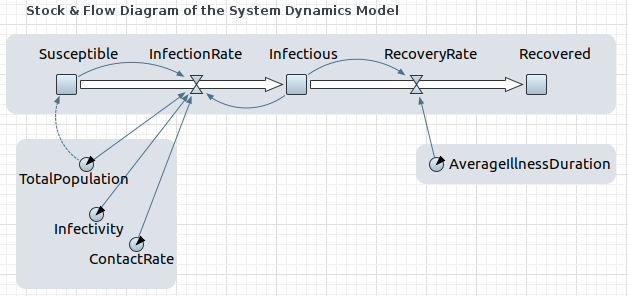
\includegraphics[width=.5\textwidth, angle=0]{./fig/SIR_SD_STOCKFLOW_DIAGRAMM.png}
	\caption{Visual System Dynamics Diagram of the SIR model in AnyLogic Personal Learning Edition 8.3.1.}
	\label{fig:sir_stockflow_diagram}
\end{figure}

Still, implementing System Dynamics directly in code is not as straight forward and involves numerical integration which can be quite tricky to get right. Thus, the aim of this paper is to look into how System Dynamics models can be implemented in code correctly without the use of a simulation package. We use the well known SIR model \cite{kermack_contribution_1927} from epidemiology to demonstrate our approach.

Our language of choice is Haskell because it emphasises a declarative programming style in which one describes \textit{what} instead of \textit{how} to compute. Further it allows to rule out interference with non-deterministic influences or side-effects already at compile-time. This is of fundamental importance for System Dynamics because it behaves completely deterministic and involves no stochastics or non-determinism whatsoever. Also, we make use of Functional Reactive Programming which allows to express continuous-time systems in a functional way. 

We show that by this approach we can arrive at correct-by-construction implementations of System Dynamic models. This means that the correctness of the code is obvious because we have closed the gap between the model specification and its implementation. Thus, the contribution of the paper is the demonstration of how to implement correct-by-construction System Dynamics simulations using Haskell and Functional Reactive Programming.

\section{Related research and literature}
\label{sec:literature}

The amount of research on using pure functional programming with Haskell in the field of ABS has been moderate so far. Most of the papers are related to the field of Multi Agent Systems (MAS) and look into how agents can be specified using the belief-desire-intention paradigm \cite{de_jong_suitability_2014,sulzmann_specifying_2007,jankovic_functional_2007}.

A multi-method simulation library in Haskell called \textit{Aivika 3} is described in the technical report \cite{sorokin_aivika_2015}. It supports implementing Discrete Event Simulations (DES), System Dynamics and comes with basic features for event-driven ABS which is realised using DES under the hood. Further it provides functionality for adding GPSS to models and supports parallel and distributed simulations. It runs within the IO effect type for realising parallel and distributed simulation but also discusses generalising their approach to avoid running in IO.

In his master thesis \cite{bezirgiannis_improving_2013} the author investigates Haskells' parallel and concurrency features to implement (amongst others) \textit{HLogo}, a Haskell clone of the NetLogo \cite{wilensky_introduction_2015} simulation package, focusing on using STM for a limited form of agent-interactions. \textit{HLogo} is basically a re-implementation of NetLogos API in Haskell where agents run within the IO context and thus can also make use of STM functionality. The benchmarks show that this approach does indeed result in a speed-up especially under larger agent-populations. The authors' thesis is one of the first on ABS using Haskell. Despite the concurrency and parallel aspect, this thesis approach is rather different: it avoids IO within the agents under all costs and explore the use of STM more on a conceptual level rather than implementing an ABS library to compare our case-studies with lock-based and imperative implementations.

There exists some research \cite{di_stefano_using_2005, varela_modelling_2004, sher_agent-based_2013} using the functional programming language Erlang \cite{armstrong_erlang_2010} to implement concurrent ABS. The language is inspired by the actor model \cite{agha_actors:_1986} and was created in 1986 by Joe Armstrong for Eriksson for developing distributed high reliability software in telecommunications. The actor model can be seen as quite influential to the development of the concept of agents in ABS, which borrowed it from Multi Agent Systems \cite{wooldridge_introduction_2009}. It emphasises message-passing concurrency with share-nothing semantics (no shared state between agents), which maps nicely to functional programming concepts. The mentioned papers investigate how the actor model can be used to close the conceptual gap between agent-specifications, which focus on message-passing and their implementation. Further they show that using this kind of concurrency allows to overcome some problems of low level concurrent programming as well.
Also \cite{bezirgiannis_improving_2013} ported NetLogos API to Erlang mapping agents to concurrently running processes, which interact with each other by message-passing. With some restrictions on the agent-interactions this model worked, which shows that using concurrent message-passing for parallel ABS is at least \textit{conceptually} feasible. Despite the natural mapping of ABS concepts to such an actor language, it leads to simulations, which despite same initial starting conditions, might result in different dynamics each time due to concurrency.

The work \cite{lysenko_framework_2008} discusses a framework, which allows to map Agent-Based Simulations to Graphics Processing Units (GPU). Amongst others they use the SugarScape model \cite{epstein_growing_1996} and scale it up to millions of agents on very large environment grids. They reported an impressive speed-up of a factor of 9,000. Although their work is conceptually very different this thesis draws inspiration from their work in terms of performance measurement and comparison to the Sugarscape model.

% THIS IS MY OWN REASEARCH, DON'T CITE IT HERE
%In \cite{thaler_pure_2019} the authors showed how to implement a spatial SIR model in pure Haskell using Functional Reactive Programming \cite{hudak_arrows_2003}. They report quite low performance but mention that STM may be a way to considerably speed up the simulation. We follow their approach in implementation technique, using Functional Reactive Programming and Monadic Stream Functions \cite{perez_functional_2016} (we don't go into implementation details as it is out of the scope of this paper) and use the spatial SIR model as the first case-study.

Using functional programming for DES was discussed in \cite{jankovic_functional_2007} where the authors explicitly mention the paradigm of Functional Reactive Programming (FRP) to be very suitable to DES.

A domain-specific language for developing functional reactive agent-based simulations was presented in \cite{schneider_towards_2012,vendrov_frabjous_2014}. This language called FRABJOUS is human readable and easily understandable by domain-experts. It is not directly implemented in FRP/Haskell but is compiled to Haskell code which they claim is also readable. This supports that FRP is a suitable approach to implement ABS in Haskell. Unfortunately, the authors do not discuss their mapping of ABS to FRP on a technical level, which would be of most interest to functional programmers.

Object-oriented programming and simulation have a long history together as the former one emereged out of Simula 67 \cite{dahl_birth_2002}, which was created for simulation purposes. Simula 67 already supported DES and was highly influential for today's object-oriented languages. Although the language was important and influential, in our research we look into different approaches, orthogonal to the existing object-oriented concepts.

Lustre is a formally defined, declarative and synchronous dataflow programming language for programming reactive systems \cite{halbwachs_synchronous_1991}. While it has solved some issues related to implementing ABS in Haskell, it still lacks a few important features necessary for ABS. There seems to be no way of implementing an environment in Lustre as it is done in Chapters \ref{ch:timedriven} and \ref{ch:eventdriven}. Also, the language seems not to come with stochastic functions, which are but the very building blocks of ABS. Finally, Lustre does only support static networks, which is clearly a drawback in ABS in general where agents can be created and terminated dynamically during simulation.

In \cite{botta_time_2010}, the authors discuss the problem of advancing time in message-driven agent-based socio-economic models. They formulate purely functional definitions for agents and their interactions through messages. Our architecture for synchronous agent-interaction as discussed in Chapter \ref{sec:eventdriven_implementation} was not directly inspired by their work but has some similarities: the use of messages and the problem of when to advance time in models which allows unrestricted synchronised agent interactions.

The authors of \cite{botta_functional_2011} are using functional programming as a specification for an agent-based model of exchange markets but leave the implementation for further research where they claim that it requires dependent types. This paper is the closest usage of dependent types in agent-based simulation we could find in the existing literature and to our best knowledge there exists no work on general concepts of implementing pure functional agent-based simulations with dependent types. %As a remedy to having no related work to build on, we looked into works which apply dependent types to solve real world problems from which we then can draw inspiration from.

In his talk \cite{sweeney_next_2006}, Tim Sweeney CTO of Epic Games discussed programming languages in the development of game engines and scripting of game logic. Although the fields of games and ABS seem to be very different, Gregory \cite{gregory_game_2018} defines computer-games as \textit{"[..] soft real-time interactive agent-based computer simulations"} (p. 9) and indeed, they have striking similarities: both are simulations which perform numerical computations and update objects in a loop either concurrently or sequential. In games these objects are called \textit{game-objects} and in ABS they are called \textit{agents} but they are conceptually the same thing.  Sweeney reports that reliability suffers from dynamic failure in languages like C++ e.g. random memory overwrites, memory leaks, accessing arrays out-of-bounds, dereferencing null pointers, integer overflow, accessing uninitialized variables. He reports that 50\% of all bugs in the Game Engine Middleware Unreal can be traced back to such problems and presents dependent types as a potential rescue to those problems. The two main points Sweeney made were that dependent types could solve most of the run-time failures and that parallelism is the future for performance improvement in games. He distinguishes between pure functional algorithms which can be parallelised easily in a pure functional language and updating game-objects concurrently using Software Transactional Memory (STM).

\chapter{Methodology}
This chapter introduces the background and methodology used in the following chapters. Roughly 50\% exists already.

\section{Agent-Based Simulation}
History, methodology (what is the purpose of ABS: 3rd way of doing science: exploratory, helps understand real-world phenomena), classification according to \cite{macal_everything_2016}, ABS vs. MAS, event- vs. time-driven \cite{meyer_event-driven_2014}, examples: agent-based SIR, SugarScape, Gintis Bartering

\subsection{Traditional approaches}
Introduce established implementation approaches to ABS. Frameworks: NetLogo, Anylogic, Libraries: RePast, DesmoJ. Programming: Java, Python, C++. Correctness: ad-hoc, manual testing, test-driven development.

\subsection{Verification \& Validation}
Introduction Verification \& Validation (V \& V in the context of ABS).

%--------------------------------------------------------------------------

\section{Pure functional programming}
Definition, Haskell references,

In our research we are using the \textit{pure} functional programming language Haskell. The paper of \cite{hudak_history_2007} gives a comprehensive overview over the history of the language, how it developed and its features and is very interesting to read and get accustomed to the background of the language. The main points why we decided to go for Haskell are:

\begin{itemize}
	\item Rich Feature-Set - it has all fundamental concepts of the pure functional programming paradigm included. Further, Haskell has influenced a large number of languages, underlining its importance and influence in programming language design.
	\item Real-World applications - the strength of Haskell has been proven through a vast amount of highly diverse real-world applications \cite{hudak_haskell_1994, hudak_history_2007}, is applicable to a number of real-world problems \cite{osullivan_real_2008} and has a large number of libraries available \footnote{\url{https://wiki.haskell.org/Applications_and_libraries}}.
	\item Modern - Haskell is constantly evolving through its community and adapting to keep up with the fast changing field of computer science. Further, the community is the main source of high-quality libraries.
	\item Purity - Haskell is a \textit{pure} functional language and in our research it is absolutely paramount, that we focus on \textit{pure} functional ABS, which avoids any IO type under all circumstances (exceptions are when doing concurrency but there we restrict most of the concepts to STM).
	\item It is as closest to pure functional programming, as in the lambda-calculus, as we want to get. Other languages are often a mix of paradigms and soften some criteria / are not strictly functional and have different purposes. Also Haskell is very strong rooted in Academia and lots of knowledge is available, especially at Nottingham, 
		Lisp / Scheme was considered because it was the very first functional programming language but deemed to be not modern enough with lack of sufficient libraries. Also it would have given the 
		Erlang was considered in prototyping and allows to map the messaging concept of ABS nicely to a concurrent language but was ultimately rejected due to its main focus on concurrency and not being purely functional.
		Scala was considered as well and has been used in the research on the Art Of Iterating paper but is not purely functional and can be also impure.
\end{itemize}


\subsection{Functional Reactive Programming}
Short introduction to FRP (yampa), based on my pure functional epidemics paper.

\subsection{Monadic Stream Functions}
Short introduction to MSFs (dunai), based on my pure functional epidemics paper.

\section{Dependent Types}
Example, Equality as Type, Philosophical Foundations: Constructive mathematics

%%%%%%%%%%%%%%%%%%%%%%%%%%%%%%%%%%%%%%%%%
% University/School Laboratory Report
% LaTeX Template
% Version 3.1 (25/3/14)
%
% This template has been downloaded from:
% http://www.LaTeXTemplates.com
%
% Original author:
% Linux and Unix Users Group at Virginia Tech Wiki 
% (https://vtluug.org/wiki/Example_LaTeX_chem_lab_report)
%
% License:
% CC BY-NC-SA 3.0 (http://creativecommons.org/licenses/by-nc-sa/3.0/)
%
%%%%%%%%%%%%%%%%%%%%%%%%%%%%%%%%%%%%%%%%%

%----------------------------------------------------------------------------------------
%	PACKAGES AND DOCUMENT CONFIGURATIONS
%----------------------------------------------------------------------------------------


\documentclass[twocolumn]{article}

\usepackage[utf8]{inputenc}
\usepackage{graphicx} % Required for the inclusion of images
\usepackage{amsmath} % Required for some math elements 
\usepackage{glossaries}
\usepackage[toc,page]{appendix}
\usepackage[autostyle=true]{csquotes}
\usepackage{hyperref}
\usepackage{amssymb}
\usepackage{caption} 
\usepackage{hhline}
\usepackage{float}
\usepackage{listings}

\setlength\parindent{0pt} % Removes all indentation from paragraphs

%\usepackage{times} % Uncomment to use the Times New Roman font

%----------------------------------------------------------------------------------------
%	DOCUMENT INFORMATION
%----------------------------------------------------------------------------------------

\title{Spec equals Code \\ Functional reactive ABS} % Title

\author{Jonathan \textsc{Thaler}} % Author name

\date{\today} % Date for the report

\begin{document}

\maketitle % Insert the title, author and date

% If you wish to include an abstract, uncomment the lines below
\begin{abstract}
The pure functional paradigm has so far got not very much attention in ABS where the dominant programming paradigm is object-orientation, realized by Java. In preliminary research of ours, we came to the insight that pure functional programming using Haskell without any additional libraries is very well suited to implement ABS but that in order to build more complex, reald-world models it would be necessary to leverage the basic concepts with functional reactive programming (FRP). In this paper we show how ABS can be fused with FRP to design an embedded domain specific language (EDSL) which allows to write specifications which (nearly) match pure functional code - the specification becomes Haskell code.
\end{abstract}

\section{Introduction}
There exists a large number of simulation packages which allow the convenient creation of System Dynamics simulations by straight-forward visual diagram creation. One simply creates stocks and flows, connects them, specifies the flow-rates and initial parameters and then runs the model. An example for such a visual diagram creation in the simulation package AnyLogic can be seen in Figure \ref{fig:sir_stockflow_diagram}.

\begin{figure}
	\centering
	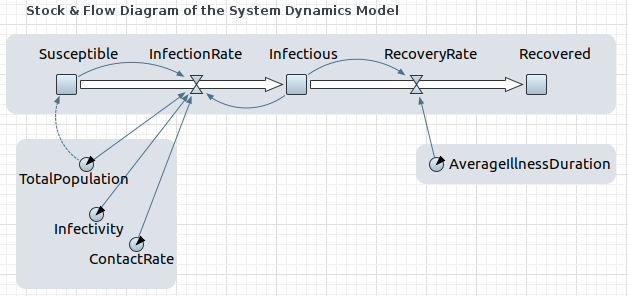
\includegraphics[width=.5\textwidth, angle=0]{./fig/SIR_SD_STOCKFLOW_DIAGRAMM.png}
	\caption{Visual System Dynamics Diagram of the SIR model in AnyLogic Personal Learning Edition 8.3.1.}
	\label{fig:sir_stockflow_diagram}
\end{figure}

Still, implementing System Dynamics directly in code is not as straight forward and involves numerical integration which can be quite tricky to get right. Thus, the aim of this paper is to look into how System Dynamics models can be implemented in code correctly without the use of a simulation package. We use the well known SIR model \cite{kermack_contribution_1927} from epidemiology to demonstrate our approach.

Our language of choice is Haskell because it emphasises a declarative programming style in which one describes \textit{what} instead of \textit{how} to compute. Further it allows to rule out interference with non-deterministic influences or side-effects already at compile-time. This is of fundamental importance for System Dynamics because it behaves completely deterministic and involves no stochastics or non-determinism whatsoever. Also, we make use of Functional Reactive Programming which allows to express continuous-time systems in a functional way. 

We show that by this approach we can arrive at correct-by-construction implementations of System Dynamic models. This means that the correctness of the code is obvious because we have closed the gap between the model specification and its implementation. Thus, the contribution of the paper is the demonstration of how to implement correct-by-construction System Dynamics simulations using Haskell and Functional Reactive Programming.

\chapter{Background}
\label{ch:background}

\section{Related research and literature}
\label{sec:literature}

The amount of research on using pure functional programming with Haskell in the field of ABS has been moderate so far. Most of the papers are related to the field of Multi Agent Systems (MAS) and look into how agents can be specified using the belief-desire-intention paradigm \cite{de_jong_suitability_2014,sulzmann_specifying_2007,jankovic_functional_2007}.

A multi-method simulation library in Haskell called \textit{Aivika 3} is described in the technical report \cite{sorokin_aivika_2015}. It supports implementing Discrete Event Simulations (DES), System Dynamics and comes with basic features for event-driven ABS which is realised using DES under the hood. Further it provides functionality for adding GPSS to models and supports parallel and distributed simulations. It runs within the IO effect type for realising parallel and distributed simulation but also discusses generalising their approach to avoid running in IO.

In his master thesis \cite{bezirgiannis_improving_2013} the author investigates Haskells' parallel and concurrency features to implement (amongst others) \textit{HLogo}, a Haskell clone of the NetLogo \cite{wilensky_introduction_2015} simulation package, focusing on using STM for a limited form of agent-interactions. \textit{HLogo} is basically a re-implementation of NetLogos API in Haskell where agents run within the IO context and thus can also make use of STM functionality. The benchmarks show that this approach does indeed result in a speed-up especially under larger agent-populations. The authors' thesis is one of the first on ABS using Haskell. Despite the concurrency and parallel aspect, this thesis approach is rather different: it avoids IO within the agents under all costs and explore the use of STM more on a conceptual level rather than implementing an ABS library to compare our case-studies with lock-based and imperative implementations.

There exists some research \cite{di_stefano_using_2005, varela_modelling_2004, sher_agent-based_2013} using the functional programming language Erlang \cite{armstrong_erlang_2010} to implement concurrent ABS. The language is inspired by the actor model \cite{agha_actors:_1986} and was created in 1986 by Joe Armstrong for Eriksson for developing distributed high reliability software in telecommunications. The actor model can be seen as quite influential to the development of the concept of agents in ABS, which borrowed it from Multi Agent Systems \cite{wooldridge_introduction_2009}. It emphasises message-passing concurrency with share-nothing semantics (no shared state between agents), which maps nicely to functional programming concepts. The mentioned papers investigate how the actor model can be used to close the conceptual gap between agent-specifications, which focus on message-passing and their implementation. Further they show that using this kind of concurrency allows to overcome some problems of low level concurrent programming as well.
Also \cite{bezirgiannis_improving_2013} ported NetLogos API to Erlang mapping agents to concurrently running processes, which interact with each other by message-passing. With some restrictions on the agent-interactions this model worked, which shows that using concurrent message-passing for parallel ABS is at least \textit{conceptually} feasible. Despite the natural mapping of ABS concepts to such an actor language, it leads to simulations, which despite same initial starting conditions, might result in different dynamics each time due to concurrency.

The work \cite{lysenko_framework_2008} discusses a framework, which allows to map Agent-Based Simulations to Graphics Processing Units (GPU). Amongst others they use the SugarScape model \cite{epstein_growing_1996} and scale it up to millions of agents on very large environment grids. They reported an impressive speed-up of a factor of 9,000. Although their work is conceptually very different this thesis draws inspiration from their work in terms of performance measurement and comparison to the Sugarscape model.

% THIS IS MY OWN REASEARCH, DON'T CITE IT HERE
%In \cite{thaler_pure_2019} the authors showed how to implement a spatial SIR model in pure Haskell using Functional Reactive Programming \cite{hudak_arrows_2003}. They report quite low performance but mention that STM may be a way to considerably speed up the simulation. We follow their approach in implementation technique, using Functional Reactive Programming and Monadic Stream Functions \cite{perez_functional_2016} (we don't go into implementation details as it is out of the scope of this paper) and use the spatial SIR model as the first case-study.

Using functional programming for DES was discussed in \cite{jankovic_functional_2007} where the authors explicitly mention the paradigm of Functional Reactive Programming (FRP) to be very suitable to DES.

A domain-specific language for developing functional reactive agent-based simulations was presented in \cite{schneider_towards_2012,vendrov_frabjous_2014}. This language called FRABJOUS is human readable and easily understandable by domain-experts. It is not directly implemented in FRP/Haskell but is compiled to Haskell code which they claim is also readable. This supports that FRP is a suitable approach to implement ABS in Haskell. Unfortunately, the authors do not discuss their mapping of ABS to FRP on a technical level, which would be of most interest to functional programmers.

Object-oriented programming and simulation have a long history together as the former one emereged out of Simula 67 \cite{dahl_birth_2002}, which was created for simulation purposes. Simula 67 already supported DES and was highly influential for today's object-oriented languages. Although the language was important and influential, in our research we look into different approaches, orthogonal to the existing object-oriented concepts.

Lustre is a formally defined, declarative and synchronous dataflow programming language for programming reactive systems \cite{halbwachs_synchronous_1991}. While it has solved some issues related to implementing ABS in Haskell, it still lacks a few important features necessary for ABS. There seems to be no way of implementing an environment in Lustre as it is done in Chapters \ref{ch:timedriven} and \ref{ch:eventdriven}. Also, the language seems not to come with stochastic functions, which are but the very building blocks of ABS. Finally, Lustre does only support static networks, which is clearly a drawback in ABS in general where agents can be created and terminated dynamically during simulation.

In \cite{botta_time_2010}, the authors discuss the problem of advancing time in message-driven agent-based socio-economic models. They formulate purely functional definitions for agents and their interactions through messages. Our architecture for synchronous agent-interaction as discussed in Chapter \ref{sec:eventdriven_implementation} was not directly inspired by their work but has some similarities: the use of messages and the problem of when to advance time in models which allows unrestricted synchronised agent interactions.

The authors of \cite{botta_functional_2011} are using functional programming as a specification for an agent-based model of exchange markets but leave the implementation for further research where they claim that it requires dependent types. This paper is the closest usage of dependent types in agent-based simulation we could find in the existing literature and to our best knowledge there exists no work on general concepts of implementing pure functional agent-based simulations with dependent types. %As a remedy to having no related work to build on, we looked into works which apply dependent types to solve real world problems from which we then can draw inspiration from.

In his talk \cite{sweeney_next_2006}, Tim Sweeney CTO of Epic Games discussed programming languages in the development of game engines and scripting of game logic. Although the fields of games and ABS seem to be very different, Gregory \cite{gregory_game_2018} defines computer-games as \textit{"[..] soft real-time interactive agent-based computer simulations"} (p. 9) and indeed, they have striking similarities: both are simulations which perform numerical computations and update objects in a loop either concurrently or sequential. In games these objects are called \textit{game-objects} and in ABS they are called \textit{agents} but they are conceptually the same thing.  Sweeney reports that reliability suffers from dynamic failure in languages like C++ e.g. random memory overwrites, memory leaks, accessing arrays out-of-bounds, dereferencing null pointers, integer overflow, accessing uninitialized variables. He reports that 50\% of all bugs in the Game Engine Middleware Unreal can be traced back to such problems and presents dependent types as a potential rescue to those problems. The two main points Sweeney made were that dependent types could solve most of the run-time failures and that parallelism is the future for performance improvement in games. He distinguishes between pure functional algorithms which can be parallelised easily in a pure functional language and updating game-objects concurrently using Software Transactional Memory (STM).

\section{Agent-Based Simulation}
\label{sec:method_abs}

%TODO RESTRUCTURING
%- classification according to \cite{macal_everything_2016}: macal paper \cite{macal_everything_2016}: very good survey/review paper on ABMS in General. fp can help with challenges h2, h4 and h5. also fp can help macals added transparency challenge, my thesis in general also adresses the knowledge challenge of macal "lack of abms educational...", note that we do NOT address ease-of-use as our approach is not easy to use. also the yampa approach can be seen as a hybrid approach of ABS/SD as posed as Research Challenge by macal. further STM might be one way of tackling large-scale ABS as identified as Research Challenge by macal. also this paper supports that ABS is a fundamentally new technique that offers the Potential to solve problems that are not robustly addressed by other methods
%\bigskip

This thesis understands ABS as a method and methodology to model and simulate a system, where the global behaviour may be unknown but the behaviour and interactions of the parts making up the system is known. Those parts, called agents, are modelled and simulated, out of which then the aggregate global behaviour of the whole system emerges. So, the central aspect of ABS is the concept of an agent, a metaphor for a pro-active unit, situated in an environment, able to spawn new agents and interacting with other agents in some neighbourhood by exchange of messages \cite{macal_everything_2016, odell_objects_2002, siebers_introduction_2008, wooldridge_introduction_2009}. Summarising, this thesis informally assumes the following about agents:

\begin{itemize}
	\item They are uniquely addressable entities with an internal state over which they have full, exclusive control.
	\item They are pro active, which means they can initiate actions on their own, for example change their internal state, send messages, create new agents, terminate themselves.
	\item They are situated in an environment and can interact with it.
	\item They can interact with other agents situated in the same environment by means of messaging.
\end{itemize} 

Epstein \cite{epstein_generative_2012} identifies ABS to be especially applicable for analysing \textit{"spatially distributed systems of heterogeneous autonomous actors with bounded information and computing capacity"}. Technically, ABS exhibits the following properties:

\begin{itemize}
	\item Linearity and non-linearity - actions of agents can lead to non-linear behaviour of the system.
	\item Time - agents act over time, which is also the source of their pro-activity.
	\item State - agents encapsulate state, which can be accessed and changed during the simulation.
	\item Feedback loop - because agents act continuously and their actions influence each other and themselves in the future of subsequent time steps, feedback loops permeate every ABS. 
	\item Heterogeneity - agents can have properties (age, height, sex,...) where the actual values can vary arbitrarily between individuals.
	\item Interactions - agents can be modelled after interactions with an environment and other agents.
	\item Spatiality and networks - agents can be situated within arbitrary environments, like spatial environments (discrete 2D, continuous 3D,...) or complex networks.
\end{itemize}

Note that there is no commonly agreed technical definition of ABS but the field draws inspiration from the closely related field of Multi-Agent Systems (MAS) \cite{weiss_multiagent_2013,wooldridge_introduction_2009}. It is important to understand that MAS and ABS are two different fields where in MAS the focus is much more on technical details, implementing a system of interacting intelligent agents within a highly complex environment with the focus primarily on solving AI problems.

\medskip

The field of ABS can be traced back to self-replicating von Neumann machines, cellular automata and Conway's Game of Life. The famous Schelling segregation model \cite{schelling_dynamic_1971} is regarded as a pioneering example. ABS as a discipline was first picked up by social simulation, which explores social norms, institutions, reputation, elections and economics. Axelrod \cite{axelrod_advancing_1997, axelrod_guide_2006} has called social simulation the third way of doing science, which he termed the \textit{generative} approach, which is in opposition to the classical inductive (finding patterns in empirical data) and deductive (proving theorems). Thus, the generative approach can be seen as a form of empirical research and is a natural environment for studying social and interdisciplinary phenomena as discussed more in depth in the work of Epstein \cite{epstein_chapter_2006, epstein_generative_2012}. He gives a fundamental introduction to agent-based social social simulation and makes the strong claim that \textit{"If you didn't grow it, you didn't explain its emergence"} \footnote{This can be seen as a fundamental constructivist approach to social science, which implies that the emergent properties are actually computable. When making connections from the simulation to reality, constructible emergence raises the question whether our existence is computable or not. When pushing this further, we can conjecture that the future of simulation will be simulated copies of our own existence, which potentially allows to simulate \textit{everything}. This idea is not new and an interesting treatment of it can be found in \cite{bostrom_are_2003, steinhart_theological_2010}.}. 
Epstein puts much emphasis on the claim that ABS is indeed a scientific instrument as hypotheses which are investigated are empirically falsifiable. If the simulation exhibits an emergent pattern, then the model is \textit{one} way of explaining it. On the other hand if it does not show the emergent pattern, then the hypothesis that the micro interactions amongst the agents generate the emergent pattern is falsified \footnote{This is fundamentally following Poppers theory of science \cite{popper_logic_2002}.} and we have not found an explanation \textit{yet}. So in summary, growing a phenomena is a necessary, but not sufficient condition for explanation \cite{epstein_chapter_2006}.

% NOTE: incorporate this only when there is enough time (and energy) to go through the 3 references cited here
%This raises a number of philosophical questions \cite{frigg_philosophy_2009}, \cite{grune-yanoff_philosophy_2010}, \cite{borrill_agent-based_2011}. Although we don't want to give an in-depth discussion of the questions raised, we want to have a quick look at them as this is a foundational research-proposal for a Doctor in \textit{Philosophy} (Ph.D.).
%TODO: read above papers and give short outline philosophical questions

The first large scale social ABS model which rose to some prominence was the \textit{Sugarscape} model developed by Epstein and Axtell in 1996 \cite{epstein_growing_1996}. Their aim was to \textit{grow} an artificial society by simulation and connect observations in their simulation to phenomenon of real-world societies. It was this simulation which strongly advertised object-oriented programming to implement ABS. Due to this influence and also due to the general popularity of the object-oriented paradigm which started to rise in the early-to-mid 90s, object-oriented programming has become the de-factor standard in implementing ABS . We can distinguish between three categories of how ABS is implemented today: % TODO: do we need citiations here to support our claims?
\begin{enumerate}
	\item Programming from scratch using object-oriented languages with Python, Java and C++ being the most popular ones.
	\item Programming using a 3rd party ABS library using object-oriented languages where RePast and DesmoJ, both in Java, are the most popular ones.
	\item Using a high-level ABS toolkit for non-programmers, which allow customisation through programming if necessary. By far the most popular one is NetLogo with an imperative programming approach followed by AnyLogic with an object-oriented Java approach.
\end{enumerate}

To get a better idea and deeper understanding of ABS, the next sections present two different, well-known agent-based models to give examples of two different types: the explanatory SIR model and the exploratory Sugarscape model. Both are used throughout the thesis as use cases for developing pure functional ABS implementation techniques, concepts and test beds for Software Transactional Memory and property-based testing.

% TODO: this is a nice blog: https://drewdevault.com/2018/07/09/Simple-correct-fast.html
% TODO: \cite{vipindeep_list_2005}
% TODO: software errors can be costly %https://raygun.com/blog/costly-software-errors-history/
% TODO: bugs per loc %https://www.mayerdan.com/ruby/2012/11/11/bugs-per-line-of-code-ratio

\input{./tex/background/sir.tex}

\input{./tex/background/sugarscape.tex}

\section{Pure Functional Programming}
\label{sec:background_fp}
To be able to understand the challenges of pure functional ABS as well as the solutions and concepts developed in this thesis, in this section we give a short introduction to functional programming, with an overview of its concepts and advanced features. As it is obviously beyond the focus of a thesis to give a full treatment of such a complex topic, we refer to additional literature and references for further discussions where appropriate.

Functional programming is called \textit{functional} because it makes functions the main concept of programming, promoting them to first-class citizens. This means that functions can be assigned to variables, they can be passed as arguments to other functions and they can be constructed as return values from functions. The roots of functional programming lie in Lambda Calculus which was first described by Alonzo Church \cite{church_unsolvable_1936}. This is a fundamentally different approach to computing than imperative programming (including established object-orientation), the roots of which lie in the Turing Machine \cite{turing_computable_1937}. Rather than describing \textit{how} something is computed as in the more operational approach of the Turing Machine, due to the more \textit{declarative} nature of Lambda Calculus, code in functional programming describes \textit{what} is computed.

In \cite{maclennan_functional_1990} the author defines functional programming as a methodology attributing the following properties to it: programming without the assignment-operator, allowing for higher levels of abstraction, allowing to develop executable specifications and prototype implementations, connected to computer science theory, performing algebraic reasoning. Further, the author makes the subtle distinction between \textit{applicative} and \textit{functional} programming. Applicative programming can be understood as applying values to functions where one deals with pure expressions. In those expressions the value is independent from the evaluation order, also known as referential transparency. This means that such functions have no side effects and thus the outcome of their execution does not depend on the history or context of the system. Additionally, inputs and effects to an operation are obvious from the written form.

Applicative programming is not necessarily unique to the functional programming paradigm but can be emulated in an imperative language like C as well. Functional programming is then defined by \cite{maclennan_functional_1990} as applicative programming with \textit{higher-order} functions. These are functions which operate themselves on functions: they can take functions as arguments, construct new functions and return them as values. This is in stark contrast to first-order functions, as used in applicative or imperative programming, which just operate on data alone. Higher-order functions allow the capturing of frequently recurring patterns in functional programming in the same way that imperative languages captured patterns like \texttt{goto}, \texttt{while-do}, \texttt{if-then-else}, \texttt{for}. Common patterns in functional programming are (amongst others) the \texttt{map}, \texttt{fold}, \texttt{zip} functions. So, functional programming is not really possible in the same way as in classic imperative languages like C, as it is not possible to construct new functions and return them as results from functions. Object-oriented languages like Java provide mechanisms allowing us to partially work around this limitation but are still far from \textit{pure} functional programming.

The equivalence in functional programming to the semicolon (;) operator of imperative programming, that allows us to compose imperative statements, is function composition. Function composition has no side effects, as opposed to the imperative semicolon operator, which simply composes destructive assignment statements executed after another, resulting in side effects.
At the heart of modern functional programming is monadic programming which is polymorphic function composition. One can implement a user-defined function composition by running code in between function composition - this code, of course, depends on the type of the Monad one runs in. This allows for emulating all kinds of effectful programming in an imperative style within a pure functional language (see Section \ref{sec:purity_sideeffects} below). Although it might seem strange following an imperative style in a pure functional language, some problems are inherently imperative in the way that computations need to be executed in a given sequence exhibiting some effects. In addition, a pure functional language needs to have some way to deal with effects, otherwise it would never be able to interact with the outside world and would be practically useless. The real benefit of monadic programming is that it is explicit about side effects and allows only effects which are fixed by the type of the Monad - the side effects which are possible are determined statically during compile time by the type system. Some general patterns can be extracted for example a \texttt{map}, \texttt{zip}, \texttt{fold} over Monads which results in effect-polymorphic behaviour. %this is the meaning when one says that a language is polymorphic in its side effects.

\subsection{Language of choice}
In our research we are using the \textit{pure} functional programming language Haskell. The paper \cite{hudak_history_2007} gives a comprehensive overview over the history of the language, how it developed and its features. The reasons for choosing Haskell are as follows:

\begin{itemize}
	\item Rich feature-set - it has all the fundamental concepts of the pure functional programming paradigm included, of which the most important ones are explained below. Moreover, Haskell has influenced a large number of languages, underlining its importance and influence in programming language design.
	
	\item Real-world applications - the strength of Haskell has been proven through a vast amount of highly diverse real-world applications \cite{hudak_history_2007, hudak_haskell_1994}. It is applicable to a number of real-world problems \cite{osullivan_real_2008} and has a large number of libraries available \cite{haskell_applications}.
	
	\item Modern - Haskell is constantly evolving through its community and adapts to keep up with the fast-paced changes in the field of computer science. Additionally, the community is the main source of high-quality libraries.
	
	\item Highly advanced type system - Haskell has a strong static type system, which catches all type errors at compile time and does not allow for bypassing the type system (unless \texttt{coerce} or other cheating functions like \texttt{unsafePerformIO} are used). In addition, Haskell is a \textit{pure} functional language and in our research it is absolutely paramount, that we focus on \textit{pure} functional ABS, which avoids any \texttt{IO} type under all circumstances. This property is enabled by the advanced type system and its strong static nature.
\end{itemize}

A highly compelling example motivating the benefits of pure functional programming is the report \cite{hudak_haskell_1994}. Where, in a prototyping contest of DARPA the Haskell prototype was by far the shortest, with 85 lines of code (LoC), as compared to the C++ solution with 1105 LoC. The remarkable thing is that the jury mistook the Haskell code as specification because its approach was to implement a small embedded domain specific language (EDSL) to solve the problem. This is a perfect proof as to how close an EDSL can get to a specification. When implementing an EDSL, one develops types and functions in a host language (embed) in a way where they can be combined. The combination of these primitives then looks like a language specific to a given domain. The ease of development of EDSLs in pure functional programming is also proof of the superior extensibility and composability of pure functional languages over object-orientation and is definitely one of its major strengths. The classic paper \cite{henderson_functional_1982} shows a wonderful way of constructing an EDSL to denotationally construct a picture reminiscent of the works of M.C.Escher. A major strength of developing an EDSL is that one can formally reason about it and do formal verification. A nice introduction about how to do reasoning in Haskell is given in \cite{hutton_tutorial_1999}.

For an excellent and widely used introduction to programming in Haskell we refer to \cite{hutton_programming_2016}. Other, more exhaustive books on learning Haskell are \cite{allen_haskell_2016, lipovaca_learn_2011}. For an introduction to programming with the Lambda-Calculus we can refer to \cite{michaelson_introduction_2011}. For a more general discussion of functional programming we refer to \cite{hudak_history_2007,hughes_why_1989,maclennan_functional_1990}.

\subsection{An Example}
Consider the factorial function in Haskell:
\begin{HaskellCode}
factorial :: Integer -> Integer
factorial 0 = 1
factorial n = n * factorial (n-1)
\end{HaskellCode}

When looking at this function, the following can be identified: 
\begin{enumerate}
	\item Declarative - describe \textit{what} the factorial function is, rather than how to compute it. This fact is supported by \textit{pattern matching} which allows providing multiple equations for the same function, matching on its input. 
	
	\item Immutable Data - in functional programming there are no mutable variables, after a variable is assigned, it cannot change its contents. This also means that there is no destructive assignment operator that can reassign values to a variable. To change values, recursion is employed.

	\item Recursion - the function calls itself with a structurally smaller argument and will eventually reach the base case of 0. Recursion is the very meat of functional programming because it is the only way to implement loops in this paradigm due to immutable data.
	
	\item Static Types - the first line indicates the name and the type of the function. In this case the function takes one Integer as input and returns an Integer as the output. Types are static in Haskell, which means that there can be no type errors at run time. For example it is not supported by this kind of type system to implicitly cast one type into another.

	\item Explicit Input and Output - all data which are required and produced by the function have to be explicitly passed in and out of it. No global mutable data exists whatsoever and data flow is always explicit.
	
	\item Referential Transparency - calling this function with the same argument will \textit{always} lead to the same result. Meaning one can replace this function by its value. Consequently, when implementing this function one cannot read from a file or open a connection to a server. This is also known as \textit{purity} and is indicated in Haskell in the types which means that it is also guaranteed by the compiler.
\end{enumerate}

It may seem that one runs into efficiency problems in Haskell when using algorithms which are implemented in imperative languages through mutable data, which allows in-place update of memory. The seminal work of \cite{okasaki_purely_1999} shows that when approaching this problem with a functional mindset, this issue will not necessarily be the case. The author presents functional data structures which are asymptotically as efficient as the best imperative implementations and discusses the estimation of the complexity of lazy programs.

\subsection{Purity and Side Effects}
\label{sec:purity_sideeffects}
One of the fundamental strengths of Haskell is its way of dealing with side effects in functions. A function with side effects has observable interactions with some state outside of its explicit scope. Therefore, its behaviour depends on the history of the system which means that it loses its referential transparency character, which makes understanding and debugging much harder. Possible examples of side effects are (amongst others): modifying a variable, awaiting an input from the keyboard, reading or writing to a file, opening a connection to a server, drawing random numbers.

Obviously, to write real-world programs which interact with the outside world requires side effects. Haskell allows for indicating in the \textit{type} of a function that it does, or does \textit{not} have side effects. What is more, there is a broad range of different effect types available, to restrict the possible effects a function can have to only the required type. This is checked by the compiler, which means that code which tries to read from a file in a function, when only allowing for drawing random numbers, will fail to compile.

A function without any side effect type is called \textit{pure}, and the \texttt{factorial} function discussed above is indeed pure. Below we give the \texttt{queryUser} function as an example of a function which is not pure. It constructs a computation, which when executed, asks the user for its user name and compares it with a given user configuration. In the event that the user name matches, it returns \texttt{True}, and \texttt{False} otherwise after printing a corresponding message. The effect type of the function is \texttt{IO}, which allows all kind of input-output related side effects like reading and writing a file, creating threads, writing to the standard output, reading from the keyboard, opening network connections and modifying mutable references.

\begin{HaskellCode}
queryUser :: String -> IO Bool
queryUser username = do
  -- print text to console
  putStr "Type in user-name: "
  -- wait for user-input
  str <- getLine
  -- check if input matches user-name
  if str == username
    then do
      putStrLn "Welcome!"			
      return True
    else do
      putStrLn "Wrong user-name!"
      return False
\end{HaskellCode}

What seems striking is that this looks very much like imperative code, which is no coincidence, but rather very much intentional. When we are dealing with side effects, ordering becomes important. Thus, Haskell introduced the so-called \textit{do} notation which emulates an imperative style of programming. Whereas, in imperative programming languages like C, instructions are chained or composed together using the semicolon (;) operator, in functional programming this is done using function composition. That is, feeding the output of a function directly into the next function. The machinery behind the \textit{do} notation does exactly this and desugars this imperative-style code into function compositions which run custom code between each line, depending on the type of effect the computation runs in. This approach of function composition with custom code in between each function allows to emulate a broad range of imperative-style effects, including the above-mentioned ones.

Although it might seem very restrictive at first, we get a number of benefits from making the type of effects we can use in a function explicit. First, we can restrict the side effects a function can have to a very specific type which is guaranteed at compile time. This means we can have much stronger guarantees about our program and the absence of potential errors immediately at compile time. Second, because running effects themselves is \textit{pure}, we can execute functions with effects in a very controlled way by making the context of the effect explicit in the parameters to the effect execution. This allows for a much easier approach to isolated testing because the history of the system is made explicit. 

\subsubsection{Monads}
Haskell implements its way of dealing with side effects using the concept of \textit{Monads}. It is important to understand that Monads are implemented directly in Haskell, which means that effects (with the exception of \texttt{IO} Monad) are implemented in terms of Haskell and not built into the runtime. To better understand how Haskell implements its concept of side effects with Monads, in this section, we briefly give an overview of what Monads are, how they are defined in Haskell and how they are used to facilitate effectful programming in a pure functional way. As this is a vast and complex topic, we can only scratch the surface here, consequently for a more technical, in-depth discussion we refer to \cite{jones_tackling_2002,moggi_computational_1989,wadler_essence_1992,wadler_monads_1995,wadler_how_1997}.

A Monad is an algebraic structure from the field of Category Theory. Moggi \cite{moggi_computational_1989} realised that Monads can be used to structure computation and later, Wadler \cite{wadler_monads_1995,wadler_how_1997} realised that Monads can be used as a way to achieve effectful computation in pure functional programming. 

Without going into the mathematical details, we give the definition of Monads in Haskell. Informally speaking, in Haskell, a Monad is both an Applicative and a Functor, which provides the operation \textit{return} and \textit{bind}. The according type class is:

\begin{HaskellCode}
-- Monad type class
-- Applicative and Functor omitted for clarity
class Applicative m => Monad m where
  return :: a -> m a
  -- bind, in Haskell >>= is used
  (>>=) :: m a -> (a -> m b) -> m b
\end{HaskellCode}

%-- Applicative type class
%-- Allows composing functions which map over values with structure.
%class Functor f => Applicative f where
%  pure  :: a -> f a
%  (<*>) :: f (a -> b) -> f a -> f b
%
%-- Functor type class
%-- Allows mapping between values with some structure.
%class Functor f where
%  fmap :: (a -> b) -> f a -> f b

\texttt{return} lifts a pure value into a Monad. \texttt{bind (>>=)} allows to sequence computations, feeding the output \texttt{a} of the first computation into a continuation, which returns a new computation in the same Monad \texttt{m} but with a possibly different return type \texttt{b}. Interestingly, with this interface it becomes possible to implement a wide range of pure, deterministic effects. As already mentioned above, in between lines of the \textit{do} notation runs custom code. This is achieved which the \texttt{bind (>>=)} method. The \texttt{return}, also seen above in the example, lifts a pure value, in the example a \texttt{Boolean} value, into a monadic value.

Obviously, the Monad type class only defines the interface required for a Monad but no actual implementations. There are a number of different Monad implementations, providing different types of side effects:

\begin{itemize}
	\item \texttt{Reader} uses partial function application to implement reading from an environment;
	\item \texttt{Writer} uses a monoid type to implement writing to a \textit{monoid} environment;
	\item \texttt{State} uses functions and closures to implement reading and writing shared state of a given type;
	\item \texttt{Rand} uses a \texttt{State} Monad to implement a random number stream;
	\item \texttt{[] (List)} forms also a Monad and implements non-deterministic programming.
\end{itemize}

To better understand how a Monad is implemented, we show the implementation of the \texttt{Maybe} Monad, which allows programming with failure. The \texttt{Maybe} type itself is straightforward and provides some kind of optional value, where a computation can either return \texttt{Just} some value or \texttt{Nothing}:

\begin{HaskellCode}
data Maybe a = Nothing | Just a
\end{HaskellCode}

Interestingly, \texttt{Maybe} forms a Monad. It allows us to write imperative-style code with the option of failure but saves us from handling each failure individually. Here is the implementation:

\begin{HaskellCode}
-- Instance of Maybe Monad.
-- Type definitions of methods provided for clarification
instance Monad Maybe where
  return :: a -> Maybe a
  return = Just
  
  (>>=) :: Maybe a -> (a -> Maybe b) -> Maybe b
  (>>=) Nothing _  = Nothing
  (>>=) (Just a) f = f a 
\end{HaskellCode}

\texttt{return} simply lifts a pure value \texttt{a} into a \texttt{Just} value, applying the data constructor \texttt{Just}. \texttt{bind (>>=)} performs case analysis: if \texttt{Maybe a} is Nothing, the it will propagate \texttt{Nothing}, otherwise it will use \texttt{a} with the continuation \texttt{f}, to return the next computation \texttt{Maybe b}.

\medskip

It is important to understand that the code fragments of effectful computations are in fact  made up of enclosing lambda expressions, with the \textit{do} notation being a syntactic sugared version. Thus functions which have an effect in their type can be seen as \textit{pure} functions, which are referentially transparent and return such a fragment. This fragment, often called \textit{action}, results in an effect and a result when executed. We have to distinguish between the execution of pure effects like \texttt{Rand}, \texttt{Read}, \texttt{Write}, \texttt{State} and the impure effect of \texttt{IO}. Pure effects are executed using special runner functions. They take an action together with one or more initial values defining the history or context of the effect - for example, an initial value for the \texttt{State} or the read-only value of the \texttt{Reader} - and then run the action returning their its value. Consequently, these pure effects can be executed in a referential transparent and completely controlled way.

However, the impure \texttt{IO} effect works differently. There is no dedicated \texttt{IO} execution function that exists, but it can only be executed from within the root \texttt{IO} action. This root action emanates from the \texttt{main :: IO ()} function of each Haskell program. As a result, \texttt{IO} actions can only be run within an enclosing \texttt{IO} action. The main \texttt{IO} action is then ultimately being executed by the Haskell runtime, which is linked against the executable. The reason for that is that if we did have a way of executing \texttt{IO} actions within pure code, we would lose all guarantees about referential transparency. The function \texttt{unsafePerformIO :: IO a $\rightarrow$ a}, exists, which allows for executing an \texttt{IO} action within a pure function, but its use is very limited and highly discouraged. Throughout this thesis and in all our code, we have avoided the use of this function at all costs. Consequently it is not used anywhere in this work, as avoiding \texttt{IO} is the very meaning of \textit{purity} and \textit{pure} functional programming.

\subsubsection{Stacking Effects}
\label{sec:back_transformers}
Often it is necessary to have multiple effects available for use. For example, if we want to manipulate a global state, write to some logging mechanism and need to be able to draw random numbers. Although Monads share a common interface and properties, it is not possible to compose Monads in general. Because each Monad has different internals and semantics, without knowing one of the two Monad to compose, it is not possible to combine them in general. Therefore, to combine two Monads, one is kept polymorphic, while the other one is known. The way this is achieved in Haskell is by using Monad Transformers \cite{allen_haskell_2016, jones_functional_1995, jones_tackling_2002}. Haskell provides the two libraries \textit{mtl} and \textit{transformers} for this, with \textit{transformers} being the older library but \textit{mtl} building on \textit{transformers}, additionally allowing for overloading functions with monadic type classes as explained below. In our approach we use both without making a distinction.

A Transformer consists of a type constructor which takes an existing Monad and returns a Monad as result. It also needs to provide implementations of both the \texttt{return} and \texttt{bind} monadic operations. Also, it needs to provide an operation \texttt{lift :: Monad m $\Rightarrow$ m a $\rightarrow$ t m a}, which allows to execute ('lift') a monadic operation \texttt{m a} from the existing Monad \texttt{m} within (into) the Transformer \texttt{t}. Therefore a Transformer is always a Monad itself, which allows for the stacking of multiple Monads or Transformers on top of each other. The stack is closed by using a non-Transformer Monad. All non-Transformer Monads are actually Transformers with the \texttt{Identity} Monad as the type parameter.

Implementing Transformers can get tricky, but as a relatively simple example, we show the implementation of the \texttt{MaybeT} Transformer from the \textit{transformers} library. The \texttt{MaybeT} is a Transformer which allows the inclusion of the \texttt{Maybe} Monad into a Transformer stack, to enable effectful computations which might fail. First, we provide the type constructor for the Transformer, which is a wrapper around the \texttt{Maybe} type, adding an arbitrary Monad \texttt{m}:

\begin{HaskellCode}
newtype MaybeT m a = MaybeT { runMaybeT :: m (Maybe a) }
\end{HaskellCode}

Then, we provide the the implementation \cite{allen_haskell_2016} of the \texttt{Monad} instance for the \texttt{MaybeT} type. Consequently, this makes \texttt{MaybeT} a Monad:

\begin{HaskellCode}
-- Instance of MaybeT Monad.
-- Type definitions of methods provided for clarification
instance (Monad m) => Monad (MaybeT m) where
  return :: a -> MaybeT a
  return = MaybeT . return . Just

  (>>=) :: MaybeT m a -> (a -> MaybeT m b) -> MaybeT m b
  (>>=) (MaybeT ma) f = MaybeT (do 
      v <- ma
      case v of
          Nothing -> return Nothing
          Just y  -> runMaybeT (f y))
\end{HaskellCode}

\texttt{return} puts the value \texttt{a} into \texttt{Just}, then lifts the \texttt{Maybe} value into the polymorphic Monad \texttt{m} and constructs a \texttt{MaybeT}. \texttt{bind (>>=)} is a bit more complex. It starts by constructing a \texttt{MaybeT} which first executes the polymorphic monadic action \texttt{ma}, resulting in a \texttt{Maybe} result. Then it performs a case analysis over the \texttt{Maybe} result. In case it is \texttt{Nothing}, it simply returns \texttt{Nothing} lifted into the polymorphic Monad \texttt{m}. In case it is \texttt{Just}, it applies the continuation \texttt{f} to get the new \texttt{MaybeT m b} value with which to construct the resulting \texttt{MaybeT}.

Finally, we provide the implementation of the \texttt{lift} operator:
 
\begin{HaskellCode}
lift :: m a -> MaybeT m a
lift = MaybeT . (liftM Just)

liftM :: Monad m => (a -> b) -> m a -> m b
\end{HaskellCode}

\texttt{lift} simply packs the value \texttt{a} into the \texttt{MaybeT m a}. It does it by using \texttt{liftM} to lift the pure data constructor \texttt{Just} into the polymorphic Monad \texttt{m}, and then constructing a \texttt{MaybeT}. Let's look at how we can define the type of a function which has multiple effects available:

\begin{HaskellCode}
data SimState = SimState { simStateAgents :: [SimAgent] ... }

simulationCore :: RandomGen g 
               => Time
               -> StateT SimState (WriterT [String] (Rand g)) SimOut
simulationCore t = do
  -- get the agents from the simulation state 
  -- encapsulated in StateT SimState
  as <- gets simStateAgents
  -- writing a logging output to the WriterT [String]
  -- here we need 1 lift 
  lift (tell ["Next step " ++ show t])
  -- shuffle agents by running the MonadRandom action using the
  -- Rand Monad, need 2 lifts as it is the innermost monad
  asShuf <- lift $ lift $ randomShuffle as
  -- construct return value
  return (SimOut { ... })
  
randomShuffle :: MonadRandom m => [a] -> m [a]
\end{HaskellCode}

The Monad stack consists of three effects. The first and \textit{outermost} effect is \texttt{StateT} with \texttt{SimState} as the internal state. As it is the outermost effect, no \texttt{lift} is required to access it. \texttt{WriterT} with \texttt{[String]} as the logging facility is a parameter to the \texttt{StateT} Transformer, making it the second effect in the stack, thus it requires one \texttt{lift}. The stack is closed using the \texttt{Rand} Monad, which is the \textit{innermost} effect, requiring two \texttt{lifts} to access it. As a result, in a Transformer stack, one needs to \textit{lift into} the stack, which means that although it is constructed inside to outside (\texttt{Rand} $\rightarrow$ \texttt{WriterT} $\rightarrow$ \texttt{StateT}) it is lifted from outside to inside (\texttt{StateT} $\rightarrow$ \texttt{WriterT} $\rightarrow$ \texttt{Rand}).

Executing a Monad Transformer stack works by using various monadic runner functions, which execute a Transformer layer with a given context as is shown in the example of section \ref{sec:back_msf} below. As with lifting, a Monad Transformer stack is evaluated from outside to inside (\texttt{StateT} $\rightarrow$ \texttt{WriterT} $\rightarrow$ \texttt{Rand}).

The function \texttt{randomShuffle} is overloaded, having the \texttt{MonadRandom} type class in its type constraints. This indicates that it is a monadic action where \texttt{m} is of type \texttt{MonadRandom}, which supports the same functionality as \texttt{Rand}. This is the major benefit mtl provides, often resulting in much cleaner function types, which do not require fixing the order of the Monads in the stack. Another benefit is that we do not need lifts anymore.The drawback is that we cannot have multiple Monads of the same type, which would be still possible in a fully qualified Monad stack. The benefits become particularly clear when more than one effect is required. For example, we can write the type of \texttt{simulationCore} as:

\begin{HaskellCode}
simulationCore :: (MonadState SimState m, MonadWriter [String] m, MonadRandom m) 
               => Time -> m SimOut
\end{HaskellCode}

A note on the commutativity of Monad Transformers: because we are stacking effects on top of each other, subsequent effects can change the final outcome, depending on their position within the stack - this is called commutativity of Monads. All the Monads in the example above commute. This means it does not matter where they are positioned in the stack, the outcome will be the same. An exception to this is the \texttt{MaybeT} Transformer, as shown above. As can be seen in the implementation, when failure occurs, subsequent effects will not be applied any more, making \texttt{MaybeT} non-commutative. Consider the following examples:

\begin{HaskellCode}
-- evaluates to: Just "Haskell" / Just 1
stateWithMaybe :: StateT Int Maybe String
stateWithMaybe = do
  modify (+1)
  return "Haskell"

-- evaluates always to Nothing
stateWithMaybeNothing :: StateT Int Maybe String
stateWithMaybeNothing = do
  modify (+1)
  lift Nothing

-- evaluates to (Just "Haskell",1)
maybeWithState :: MaybeT (State Int) String
maybeWithState = do
  lift $ modify (+1)
  return "Haskell"

-- evaluates to (Nothing,1)
maybeWithStateFail :: MaybeT (State Int) String
maybeWithStateFail = do
  lift $ modify (+1)
  fail "Some Failure"
\end{HaskellCode}

Depending on whether we want the \texttt{String} returned by the computation or the \texttt{Int} of the \texttt{StateT}, \texttt{stateWithMaybe} evaluates always to some \texttt{Just} value. However, \texttt{stateWithMaybeNothing} \textit{always} evaluates to \texttt{Nothing}, discharging the \texttt{Int} state of the \texttt{StateT}.

\texttt{maybeWithState} always evaluates to \texttt{(Just "Haskell",1)}: it returns \textit{both} the final value of the \texttt{State} \textit{and} the \texttt{String} returned by the computation. This makes it possible that \texttt{maybeWithStateFail} fails, therefore returning no \texttt{String} but still retaining the state of the \texttt{State} effect.

\subsection{Functional Reactive Programming}
\label{sec:back_frp}
Functional Reactive Programming (FRP) is a way to implement systems with continuous and discrete time semantics in pure functional languages. There are many different approaches and implementations but, in this thesis, \textit{Arrowized} FRP \cite{hughes_generalising_2000, hughes_programming_2005} as implemented in the library Yampa \cite{courtney_yampa_2003,hudak_arrows_2003,nilsson_functional_2002} and Dunai \cite{perez_functional_2016} (see below) is used.

The central concept in Arrowized FRP is the signal function (SF), which can be understood as a \textit{process over time} which maps an input- to an output signal. A signal can be understood as a value which varies over time. Therefore, signal functions have an awareness of the passing of time by having access to $\Delta t$ which are positive time steps, the system is sampled with:

\begin{flalign*}
Signal \, \alpha \approx Time \rightarrow \alpha \\
SF \, \alpha \, \beta \approx Signal \, \alpha \rightarrow Signal \, \beta 
\end{flalign*}

Yampa provides a number of combinators for expressing time semantics, events and state changes of the system. They allow to change system behaviour in case of events, run signal functions and generate stochastic events and random-number streams. Below, the relevant combinators and concepts used throughout the thesis are discussed briefly. For a more in-depth discussion we refer to \cite{courtney_yampa_2003, hudak_arrows_2003, nilsson_functional_2002} in the reference section.

\paragraph{Event}
An event in FRP is an occurrence at a specific point in time, which has no duration. An example of such an event would be the recovery of an infected agent. Yampa represents events through the \texttt{Event} type, which is programmatically equivalent to the \texttt{Maybe} type. 

\paragraph{Dynamic behaviour}
To change the behaviour of a signal function at an occurrence of an event during run time, (amongst others) the combinator \texttt{switch :: SF a (b, Event c) $\rightarrow$ (c $\rightarrow$ SF a b) $\rightarrow$ SF a b} is used. It takes a signal function, which is run until it generates an event. When this event occurs, the function in the second argument is evaluated, which receives the data of the event and has to return the new signal function. This new signal function will then replace the previous one. The semantics of \texttt{switch} are that the signal function, into which is switched, is also executed at the time of switching.

\paragraph{Randomness}
In ABS, often there is the need to generate stochastic events, which occur based on a certain distribution. Yampa provides the combinator \texttt{occasionally :: RandomGen g $\Rightarrow$ g $\rightarrow$ Time $\rightarrow$ b $\rightarrow$ SF a (Event b)} for this. It takes a random-number generator, a rate and a value the stochastic event will carry. It generates events on average with the given rate, following the exponential distribution. At most, one event will be generated and no backlog is kept. This means that when this function is not sampled with a sufficiently high frequency, depending on the rate, it will lose events.

Yampa also provides the combinator \texttt{noise :: (RandomGen g, Random b) $\Rightarrow$ g $\rightarrow$ SF a b}, which generates a stream of noise by returning a random number in the default range for the type \texttt{b}, following the uniform distribution.

\paragraph{Running signal functions}
To run a signal function Yampa provides the function \texttt{embed :: SF a b $\rightarrow$ (a, [(DTime, Maybe a)]) $\rightarrow$ [b]}, which allows for running an SF for a given number of steps. Where, in each step one provides the $\Delta t$ and an input \texttt{a}. The function then returns the output of the signal function for each step. The input is optional, indicated by \texttt{Maybe}. In the first step at $t = 0$, the initial \texttt{a} is applied and whenever the input is \texttt{Nothing} in subsequent steps, the last \texttt{a} which was not \texttt{Nothing} is reused.

\subsection{Arrowized programming}
Yampa's signal functions are Arrows, requiring us to program with Arrows. Arrows are a generalisation of Monads, which in addition to the already familiar parameterisation over the output type, allow parameterisation over their input type as well \cite{hughes_generalising_2000, hughes_programming_2005}. For a clearer understanding, we show how Arrows are defined in terms of Haskell \cite{arrows_haskell}:

\begin{HaskellCode}
class Arrow a where
  -- Each function may be treated as a computation.  
  arr :: (b -> c) -> a b c
  
  -- A computation applied to part of the input, 
  -- with the rest copied through to the output.
  first :: a b c -> a (b,d) (c,d)
  
  -- Computations may be composed, by connecting 
  -- the output of the first to the input of the second.
  (>>>) :: a b c -> a c d -> a b d
\end{HaskellCode}

It is clear to see in the type definitions, that each method also parametrises over the input type. As a simple example for an Arrow instance we provide the implementation of an Arrow for pure function computations:

\begin{HaskellCode}
newtype Func a b = Func { runFunc :: (a -> b) }

-- Instance of pure function computations as Arrow.
-- Type definitions of methods provided for clarification
instance Arrow Func where
  arr :: Func a b
  arr f = Func f

  first :: Func b c -> Func (b, d) (c, d)
  first (Func f) = Func (mapFst f)
    where
      mapFst g (a,b) = (g a, b)
    
  (>>>) :: Func b c -> Func c d -> Func b d
  (>>>) (Func f) (Func g) = Func (g . f)
\end{HaskellCode}

In general, Arrows can be understood to be computations that represent processes, which take an input of a specific type, process it and output a value of a given type. This is also reflected in the types of the \texttt{Arrow} type class and the example above: we are dealing with functions and not individual arguments, as in the case of Monads. The concept of processes, which signal functions indeed are, maps naturally to Arrows which is the reason why Yampa is using them to represent their signal functions.

There exists a number of Arrow combinators, which allow arrowized programming in a point-free style but due to lack of space we will not discuss them here. Instead we make use of Paterson's \textit{do} notation for arrows \cite{paterson_new_2001}, which makes the code more readable as it allows us to program with points.

To show how arrowized programming works, we implement a simple signal function, which calculates the acceleration of a falling mass on its vertical axis as an example \cite{perez_testing_2017}.

\begin{HaskellCode}
fallingMass :: Double -> Double -> SF () Double
fallingMass p0 v0 = proc _ -> do
  v <- arr (+v0) <<< integral -< (-9.8)
  p <- arr (+p0) <<< integral -< v
  returnA -< p
\end{HaskellCode}

To create an Arrow, the \texttt{proc} keyword is used, which binds a variable after which the \texttt{do} of Patersons \textit{do} notation \cite{paterson_new_2001} follows. Using the signal function \texttt{integral :: SF v v} of Yampa, which integrates the input value over time using the rectangle rule, we calculate the current velocity and the position based on the initial position \texttt{p0} and velocity \texttt{v0}. The \texttt{<<<} is one of the Arrow combinators, which composes two Arrow computations and \texttt{arr} simply lifts a pure function into an Arrow. To pass an input to an Arrow, \texttt{-<} is used and \texttt{<-} is used to bind the result of an Arrow computation to a variable. Finally to return a value from an Arrow, \texttt{returnA} is used.

\subsection{Monadic Stream Functions}
\label{sec:back_msf}
Monadic Stream Functions (MSF) are a generalisation of Yampa's signal functions but they have additional combinators to control and stack side effects. An MSF is a polymorphic type and an evaluation function, which applies an MSF to an input and returns an output and a continuation, both in a monadic context \cite{perez_extensible_2017,perez_functional_2016}:
\begin{HaskellCode}
newtype MSF m a b = MSF {unMSF :: MSF m a b -> a -> m (b, MSF m a b)}
\end{HaskellCode}

An MSF is also an Arrow, which means we can apply arrowized programming with Patersons \textit{do} notation as well. MSFs are implemented in Dunai, which is available on Hackage \cite{dunai_library}. Dunai allows for the application of monadic transformations by means of combinators like \texttt{arrM :: Monad m $\Rightarrow$ (a $\rightarrow$ m b) $\rightarrow$ MSF m a b} and \texttt{arrM\_ :: Monad m $\Rightarrow$ m b $\rightarrow$ MSF m a b}. A part of the library Dunai is BearRiver, a wrapper, which reimplements Yampa on top of Dunai. This wrapper enables one to run arbitrary monadic computations in a signal function. BearRiver simply adds a type parameter \texttt{m} to each \texttt{SF}, which indicates the monadic context in which this signal function runs.

To show how arrowized programming with MSFs works, we extend the falling mass example from above to incorporate effects. In this (artificial) example we assume that in each step we want to accelerate our velocity \texttt{v} not by the gravity constant anymore but by a random number in the range of 0 to 9.81. Moreover, we want to count the number of steps it takes us to hit the floor, that is, when the position \texttt{p} is less than 0. Additionally, when hitting the floor we want to print a debug message to the console with the velocity, by which the mass has hit the floor and how many steps it took.

We define a corresponding Monad stack with \texttt{IO} as the innermost Monad to print to the console, followed by a \texttt{RandT} Transformer for drawing random numbers, and finally, a \texttt{StateT} Transformer as the outermost Monad, to count the number of steps we compute. We can access the monadic functions using \texttt{arrM} in case we need to pass an argument, and \texttt{\_arrM}, in case no argument to the monadic function is needed:

\begin{HaskellCode}
type FallingMassStack g = StateT Int (RandT g IO)
type FallingMassMSF g   = SF (FallingMassStack g) () Double

fallingMassMSF :: RandomGen g => Double -> Double -> FallingMassMSF g
fallingMassMSF v0 p0 = proc _ -> do
  -- drawing random number for our gravity range
  r <- arrM_ (lift $ lift $ getRandomR (0, 9.81)) -< ()
  v <- arr (+v0) <<< integral -< (-r)
  p <- arr (+p0) <<< integral -< v
  -- count steps
  arrM_ (lift (modify (+1))) -< ()
  if p > 0
    then returnA -< p
    -- we have hit the floor
    else do
      -- get number of steps
      s <- arrM_ (lift get) -< ()
      -- write to console
      arrM (liftIO . putStrLn) -< "hit floor with v " ++ show v ++ 
                                  " after " ++ show s ++ " steps"
      returnA -< p
\end{HaskellCode}

To run the \texttt{fallingMassMSF} function until it hits the floor we proceed as follows:

\begin{HaskellCode}
runMSF :: RandomGen g => g -> Int -> FallingMassMSF g -> IO ()
runMSF g s msf = do
  let msfReaderT = unMSF msf ()
      msfStateT  = runReaderT msfReaderT 0.1 -- sampling with time delta of 0.1
      msfRandT   = runStateT msfStateT s
      msfIO      = runRandT msfRandT g
  (((p, msf'), s'), g') <- msfIO
  when (p > 0) (runMSF g' s' msf')
\end{HaskellCode}

Dunai does not know about time in MSF, which is exactly what BearRiver builds on top. It does so by adding a \texttt{ReaderT Double}, which carries the $\Delta t$. This is the reason why we need one extra lift for accessing \texttt{StateT} and \texttt{RandT}. Thus, \texttt{unMSF} returns a computation in the \texttt{ReaderT Double} Monad, which we need to peel away using \texttt{runReaderT}. This action then results in a \texttt{StateT Int} computation, which we evaluate by using \texttt{runStateT} and the current number of steps as state. This then results in another monadic computation of \texttt{RandT} Monad, which we evaluate using \texttt{runRandT}. This finally returns an \texttt{IO} computation, which we simply evaluate to arrive at the final result.

As explained in the previous section \ref{sec:back_transformers}, this example shows how a Monad Transformer stack is lifted and evaluated from outside to inside (\texttt{ReaderT} $\rightarrow$ \texttt{StateT} $\rightarrow$ \texttt{RandT} $\rightarrow$ \texttt{IO}) but constructed inside to outside (\texttt{IO} $\rightarrow$ \texttt{RandT} $\rightarrow$ \texttt{StateT} $\rightarrow$ \texttt{ReaderT}).

\section{Methodology}
%- Methodology is the justification for using a particular research method.
%- make clear what our method is (Method is simply a research tool, a component of research – say for example, a qualitative method such as interviews) and then justify it => this is then the methodology 
%- discussion of methodology is missing: what is the scientific approach we used in our thesis to address the aims and answer hypotheses? Basically we perform use-cases and discuss them\\

In this section we briefly motivate and justify our methods, to point out the scientific approach used in this thesis to address the aims and answer hypotheses put forward in Chapter \ref{ch:intro}. Fundamentally, the method we use is developing concepts step-by-step using the two well known agent-based models SIR, introduced in Chapter \ref{sec:sir_model} and Sugarscape, introduced in Chapter \ref{sec:sugarscape}. We put our approach into a broader context of how to implement ABS from a programming language agnostic view, discussed in Chapter \ref{ch:impl_abs}, which serves as underlying assumptions and general direction to follow.

The first part of our method is dedicated to answer the question of how to implement ABS in a pure functional way, following a time-driven approach in Chapter \ref{ch:timedriven} and an event-driven approach in Chapter \ref{ch:timedriven}. The reason for two techniques is that both are equally important in ABS and also that the concepts of event-driven ABS build on the ones developed in the preceding time-driven approach.

Generally, in both approaches, the aim is to develop a robust, maintainable and extensible implementation of the use-case models through which we develop concepts which can be adopted to ABS in general. The overall goal is a clear representation of agents with their local (immutable) state, a way for the agents to interact with an (active) environment and one-directional and synchronous interactions between agents. 

In the process of researching the pure functional event-driven approach to ABS, we also undertook a full and validated implementation of the Sugarscape model. This in itself together with the concepts developed, is already a sufficient proof that using a pure functional language to implement non-trivial ABS models is possible in a robust and maintainable way.

%It is quite important to state this clearly as we could follow a rather completely data-driven approach, which would have been very easy in pure functional programming: represent all agents and the simulation state as a big data-structure which is passed in and out pure functions (thus read/write). Indeed it would work but we would probably end up in a difficult to understand data-flow (everything is read/write) and what is worse: we don't arrive at very general solutions as we would not abstract out concepts, existing in ABS already which could then be transferred easily. Note that a more data-driven approach has indeed its value, depending on the model! In Chapter \ref{ch:gintis_case} we briefly introduce the field of ACE, where agents are almost always completely represented by data and very simple behaviour and do not interact in a complex way as in Sugarscape. Examples are ZI traders or bilateral traders which are all simply represented by data and interact with each other quite indirectly through a trading and bartering process.

The second part of our method is dedicated to show the benefits of using the previously developed pure functional approach to ABS. It is split into two parts where in the first we investigate the hypothesis that pure functional programming makes it easy to apply parallel computation using parallelism and concurrency to ABS. The second part answers another central hypothesis namely that randomised property-based testing is a good match to test stochastic ABS implementations. In both parts we apply the concepts in questions directly to the implementations developed in the previous part and look at the resulting code, performance and implications to judge whether the outcome has the expected benefit or not as stated in the hypotheses.

Generally, all concepts we derive are driven by the hypotheses and aims from the Introduction and we continuously refer back to them, especially in the respective discussions and the final conclusion and discussion chapters. By doing this we are able to qualitatively assess whether the thesis has achieved the initial aims and answered the hypotheses in a satisfactory way.

\section{The formal Agent-Model}

TODO: define an agent 

%\documentclass[a4paper, 10pt, conference]{../../templates/IEEEconf/IEEEconf}
\documentclass[10pt, conference, onecolumn]{../../papers/templates/IEEEtran/IEEEtran}
%\documentclass[10pt, journal]{../../templates/IEEEtran/IEEEtran}

\usepackage{graphicx}
\usepackage{caption} 
\usepackage{subcaption}
\usepackage{hyperref}
\usepackage{listings}
\usepackage{hhline}
\usepackage{float}
\usepackage{amssymb}
\usepackage[autostyle=true]{csquotes}
\usepackage{amsmath}
\usepackage{marvosym}
\usepackage{minted}

\font\subtitlefont=cmr12 at 18pt

% First Contact
\title{Functional Reactive Agent-Based Simulation}

% IEEEtran journal authors
%\author{Jonathan Thaler, ̃Peer-Olaf Siebers \\ School of Computer Science \\ University of Nottingham%
%\thanks{jonathan.thaler@nottingham.ac.uk}%
%\thanks{peer-olaf.siebers@nottingham.ac.uk}
%}

% IEEEtran conference authors
\author{
	\IEEEauthorblockN{Jonathan Thaler}
	\IEEEauthorblockA{School of Computer Science\\
		University of Nottingham\\
		jonathan.thaler@nottingham.ac.uk}
		
	\and
		
	\IEEEauthorblockN{Thorsten Altenkirch}
	\IEEEauthorblockA{School of Computer Science\\
		University of Nottingham\\
		thorsten.altenkirch@nottingham.ac.uk}
}

%\IEEEpubid{0000--0000/00\$00.00 ̃\copyright ̃2015 IEEE}

% IEEEconf authors
%\author{
%	Jonathan Thaler \\
%	\email{jonathan.thaler@nottingham.ac.uk} \\
%	\begin{affiliation}
%		School of Computer Science, University of Nottingham
%	\end{affiliation} \\
%	\and 
%	Peer-Olaf Siebers \\
%	\email{peer-olaf.siebers@nottingham.ac.uk} \\
%	\begin{affiliation}
%		School of Computer Science, University of Nottingham
%	\end{affiliation} 
%	\and 
%	Thorsten Altenkirch \\
%	\email{thorsten.altenkirch@nottingham.ac.uk} \\
%	\begin{affiliation}
%		School of Computer Science, University of Nottingham
%	\end{affiliation} 
%}

\begin{document}
\maketitle 

\begin{abstract}
TODO: feedback by thorsten: its too hardcore! instead of presenting my library we need to do "how to arrive at FrABS from Haskell to Yampa to FrABS" in which we (thorsten and me) derive step-by-step an implementation of a very simple agent-based model using Haskell and Yampa. The conclusion will then be that we provide all stuff already in FrABS. 
TODO: split the approach to FrABS into the following steps
	1.: run in random monad without any reactive features. problem: need to drag time \& state around, also need to feedback state into all agents
	2.: run in Yampa with reactive features. problem: randomness is tedious, still feedback of state into all
	3.: run in Dunai.
	
TODO: need to select the right journal for publication, something more practical functional programming

TODO: pictures should show up where they are mentioned in the text

TODO: cite my own 1st paper from SSC2017: add it to citations

TODO: refine it: start with simulating epidemics and then go into ABS

Agent-Based Simulation (ABS) is a methodology in which a system is simulated in a bottom-up approach by modelling the micro interactions of its constituting parts, called agents, out of which the global macro system behaviour emerges. So far, the Haskell community hasn't been much in contact with the community of ABS due to the latter's primary focus on the object-oriented programming paradigm. This paper tries to bridge the gap between those two communities by introducing the Haskell community to the concepts of ABS. We do this by deriving an agent-based implementation for the simple SIR model from epidemiology. In our approach we leverage the basic concepts of ABS with functional reactive programming from Yampa which results in a surprisingly fresh, powerful and convenient EDSL for formulating ABS in Haskell.
\end{abstract}

\begin{IEEEkeywords}
Functional Reactive Programming, Agent-Based Simulation
\end{IEEEkeywords}

\section{Introduction}
There exists a large number of simulation packages which allow the convenient creation of System Dynamics simulations by straight-forward visual diagram creation. One simply creates stocks and flows, connects them, specifies the flow-rates and initial parameters and then runs the model. An example for such a visual diagram creation in the simulation package AnyLogic can be seen in Figure \ref{fig:sir_stockflow_diagram}.

\begin{figure}
	\centering
	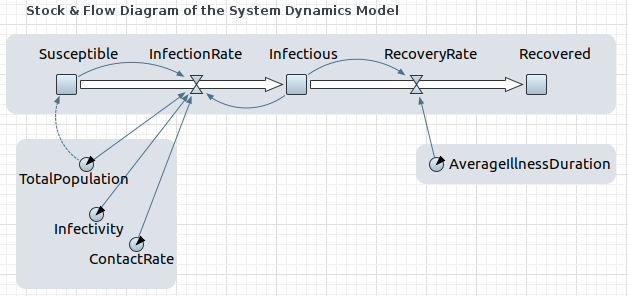
\includegraphics[width=.5\textwidth, angle=0]{./fig/SIR_SD_STOCKFLOW_DIAGRAMM.png}
	\caption{Visual System Dynamics Diagram of the SIR model in AnyLogic Personal Learning Edition 8.3.1.}
	\label{fig:sir_stockflow_diagram}
\end{figure}

Still, implementing System Dynamics directly in code is not as straight forward and involves numerical integration which can be quite tricky to get right. Thus, the aim of this paper is to look into how System Dynamics models can be implemented in code correctly without the use of a simulation package. We use the well known SIR model \cite{kermack_contribution_1927} from epidemiology to demonstrate our approach.

Our language of choice is Haskell because it emphasises a declarative programming style in which one describes \textit{what} instead of \textit{how} to compute. Further it allows to rule out interference with non-deterministic influences or side-effects already at compile-time. This is of fundamental importance for System Dynamics because it behaves completely deterministic and involves no stochastics or non-determinism whatsoever. Also, we make use of Functional Reactive Programming which allows to express continuous-time systems in a functional way. 

We show that by this approach we can arrive at correct-by-construction implementations of System Dynamic models. This means that the correctness of the code is obvious because we have closed the gap between the model specification and its implementation. Thus, the contribution of the paper is the demonstration of how to implement correct-by-construction System Dynamics simulations using Haskell and Functional Reactive Programming.

\section{Defining Agent-Based Simulation}
Agent-Based Simulation (ABS) is a methodology to model and simulate a system where the global behaviour may be unknown but the behaviour and interactions of the parts making up the system is of knowledge. Those parts, called agents, are modelled and simulated out of which then the aggregate global behaviour of the whole system emerges. So the central aspect of ABS is the concept of an agent which can be understood as a metaphor for a pro-active unit, situated in an environment, able to spawn new agents and interacting with other agents in some neighbourhood by exchange of messages \cite{wooldridge_introduction_2009}. We informally assume the following about our agents:

\begin{itemize}
	\item They are uniquely addressable entities with some internal state over which they have full, exclusive control.
	\item They are pro-active which means they can initiate actions on their own e.g. change their internal state, send messages, create new agents, terminate themselves.
	\item They are situated in an environment and can interact with it.
	\item They can interact with other agents which are situated in the same environment by means of messaging.
\end{itemize} 

Epstein \cite{epstein_generative_2012} identifies ABS to be especially applicable for analysing \textit{"spatially distributed systems of heterogeneous autonomous actors with bounded information and computing capacity"}. Thus in the line of the simulation types \textit{Statistic} $^\dag$, \textit{Markov} $^\ddag$, \textit{System Dynamics} $^\S$, \textit{Discrete Event} $^\mp$, ABS is the most powerful one as it allows to model  the following:

\begin{itemize}
	\item Linearity \& Non-Linearity $^{\dag \ddag \S \mp}$ - the dynamics of the simulation can exhibit both linear and non-linear behaviour. 
	\item Time $^{\dag \ddag \S \mp}$ - agents act over time, time is also the source of pro-activity.
	\item States $^{\ddag \S \mp}$ - agents encapsulate some state which can be accessed and changed during the simulation.
	\item Feedback-Loops $^{\S \mp}$ - because agents act continuously and their actions influence each other and themselves, feedback-loops are the norm in ABS. 
	\item Heterogeneity $^{\mp}$ - although agents can have same properties like height, sex,... the actual values can vary arbitrarily between agents.
	\item Interactions - agents can be modelled after interactions with an environment or other agents, making this a unique feature of ABS, not possible in the other simulation models.
	\item Spatiality \& Networks - agents can be situated within e.g. a spatial (discrete 2d, continuous 3d,...) or network environment, making this also a unique feature of ABS, not possible in the other simulation models.
\end{itemize}

\section{The SIR Model}
To explain the concepts of ABS and of our functional reactive approach to it, we introduce the SIR model as a motivating example. The SIR model is a a very well studied and understood compartment model from epidemiology which allows to simulate the dynamics of an infectious disease spreading through a population. In this model, people in a population of size $N$ can be in either one of three states \textit{Susceptible}, \textit{Infected} or \textit{Recovered} at a particular time, where it is assumed that initially there is at least one infected person in the population. People interact with each other \textit{on average} with a given rate $\beta$ per time-unit and get infected with a given probability $\gamma$ when interacting with an infected person. When infected, a person recovers \textit{on average} after $\delta$ time-units and is then immune to further infections. An infected person interaction with another infected one is never re-infected, thus interactions amongst infected people is not important in this model. This definition gives rise to three compartments with the transitions as seen in Figure \ref{fig:sir_transitions}.

\begin{figure}
	\centering
	
\includegraphics[width=.4\textwidth, angle=0]{./fig/SIR_transitions.png}
	\caption{Transitions in the SIR compartment model.}
	\label{fig:sir_transitions}
\end{figure}

The dynamics of this model over time can be formalized using the following equations:

$\frac{\mathrm d S}{\mathrm d t} = -infectionRate$ \\
$\frac{\mathrm d I}{\mathrm d t} = infectionRate - recoveryRate$ \\
$\frac{\mathrm d R}{\mathrm d t} = recoveryRate$ \\

$infectionRate = \frac{I \beta S \gamma}{N}$ \\
$recoveryRate = \frac{I}{\delta}$ \\

Solving these can be done using the System-Dynamics (SD) approach which solves the equations by integrating over time. In the SD terminology, the intergrals are called \textit{Stocks} and the values over which is integrated over time are called \textit{Flows}.

$S(t) = N + \int_0^t -infectionRate\, \mathrm{d}t$ \\
$I(t) = 1 + \int_0^t infectionRate - recoveryRate\, \mathrm{d}t$ \\
$R(t) = \int_0^t recoveryRate\, \mathrm{d}t$ \\

There exist a huge number of software-packages which allow to conveniently express SD models using a visual approach like in Figure \ref{fig:sir_sd_stockflow_diagramm}.

\begin{figure}
	\centering
	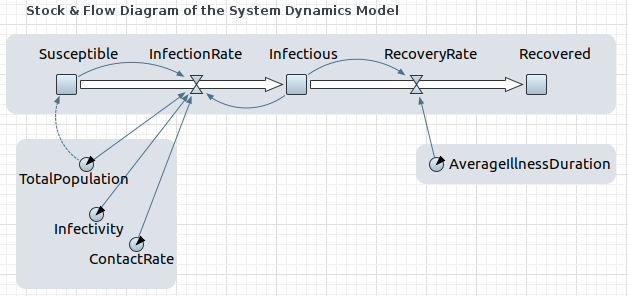
\includegraphics[width=.4\textwidth, angle=0]{./fig/SIR_SD_STOCKFLOW_DIAGRAMM.png}
	\caption{A visual representation of the stocks and flows in the SIR compartment model (Image courtesy of AnyLogic Company).}
	\label{fig:sir_sd_stockflow_diagramm}
\end{figure}

Running the SD simulation over time results in the dynamics as shown in Figure \ref{fig:sir_sd_dynamics_anylogic} with the given variables.

\begin{figure}
	\centering
	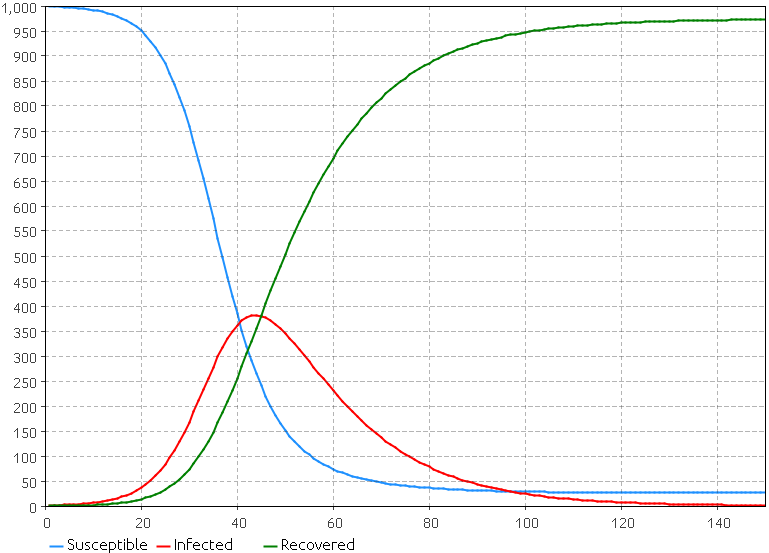
\includegraphics[width=.4\textwidth, angle=0]{./fig/SIR_SD_DYNAMICS_ANYLOGIC.png}
	\caption{Dynamics of the SIR compartment model using the System Dynamics approach generated with the AnyLogic Personal Learning Edition 8.1.0. Population Size $N$ = 1000, contact rate $\beta = 1/5$, infection probability $\gamma = 0.05$, illness duration $\delta = 15$.}
	\label{fig:sir_sd_dynamics_anylogic}
\end{figure}

\subsection{An Agent-Based approach}
The SD approach is inherently Top-Down because the emergent property of the system is formalized in differential equations. The question is if such a top-down behaviour can be emulated using ABS, which is inherently bottom-up. Also the question is if there are fundamental drawbacks and benefits when doing so using ABS. Indeed such questions were asked before and modelling the SD approach of the SIR model is possible using an agent-based approach. It is important to note that SD treats the population completely continuous which results in non-discrete values of stocks e.g. 3.1415 infected persons. Thus the fundamental approach to map the SIR model to an ABS is to discretisize the population and model each person in the population as an invidivual agent. The transition  between the states are no longer happening according to continuous differential equations but due to discrete events caused both by interactions amongst the agents and time-outs. The behaviour can be defined as follows:

\begin{itemize}
	\item Every agent makes on average contact with $\beta$ random other agents per time unit. In ABS we can only contact discrete agents thus we model this by generating a random event on average every $\beta$ time units.
	
	\item An agent does not know the other agents state when making contact with it, thus we need a mechanism in which agents reveal their state in which they are in \textit{at the moment of making contact}. Obviously the already mentioned messaging-mechanism which allows agents to interact is perfectly suited to do this.
	\begin{itemize}
		\item \textit{Susceptible} agent: sends a "Susceptible" message when contacting another agent. There is no need to reply to other incoming messages as making contact with a susceptible agent has no influence on the state of an agent.
		\item \textit{Infected} agent: sends a "Infected" message when contacting another agent. An infected agent now needs to reply to incoming "Susceptible" messages with an "Infected" message to let the susceptible agent know that it has made contact with an infected agent.
		\item \textit{Recovered} agent: does not need to send messages because contacting it or being contacted by it has no influence on the state.
	\end{itemize}
	
	\item Susceptible to Infected: needs to have made contact with an infected agent which happens when it receives an "Infected" message. If this occurs an infection occurs with a probability of $\gamma$. The infection can be calculated by drawing from a uniform random-distribution between 0 and 1 and comparing the value to $\gamma$, if the drawn value $p < \gamma$ then infection occurs. Note that this needs to be done for \textit{every} received "Infected" message.
	
	\item Infected to Recovered: a person recovers \textit{on average} after $\delta$ time unites. This is implemented by drawing the duration from an exponential distribution (TODO: borchschev) with $\lambda = \frac{1}{\delta}$ and making the transition after this duration.
\end{itemize}

We will discuss the implementation of this approach in the following sections and as will be shown FrABS will allow us to express this behaviour very explicitly looking very much like a formal ABS specification of the problem. For now we will give the resulting dynamics in Figure TODO

TODO: how many initially infected agents? one should be enough, at least in my implementation

TODO: 100 vs. 1000 vs. 5.000 agents

TODO: problem in my code: need exponentially occasionally not uniform distributed! => OK, occasionally draws from exponential-distribution
TODO: what differences do the different update strategies make?

\subsection{Blub}
TODO: It should be possible to formally show that spatial SIR and WildFire are the same model. NOTE: they are NOT the same, the fundamental difference is that in the WildFire model only the burning cells initiate the ignition - if we compare this to the SIR, the burning cells would be infected agents and although in the spatial SIR model the infected agents make contact with other agents, so do the susceptible ones which does NOT occur in wildfire

TODO: cite my own work on update-strategies

TODO: can we formally show that the SIR approximates the SD model?

TODO: cite papers which discuss how to approximate a SD model by ABS
- Macal (2010) - To Agent-Based Simulation From System Dynamics 
	-> i am very unhappy with this paper: first it does not give concrete parameters for the SD model so it is impossible to replicate. Also i think it has a systematical error as the infected agents make no contact but this is required as evident from the SD-models infection-rate which also incorporates. TODO: write an email to this guy: why are the infectious not contacting the other agents? this seems to be a systematical error
- Borshchev, Filippov (2004) - From System Dynamics and Discrete Event to Practical Agent Based Modeling: Reasons, Techniques, Tools
	-> its VERY IMPORTANT point is that we need to draw the illness-duration from an exponential-distribution because the illness-duration is proportional to the size of the infected. note: this is wrongly expressed, need to find the correct formulation

		-> my emulation of SD using ABS is really an implementation of the SD model and follows it - they are equivalent
		-> my ABS implementation is the same as / equivalent to the SD emulation
			=> thus if i can show that my SD emulation is equlas to the SD model
			=> AND that the ABS implementation is the same as the SD emulation
			=> THEN the ABS implementation is an SD implementation, and we have shown this in code for the first time in ABS
			


\section{Functional Reactive ABS}
%TODO: cross reference to the code in the appendix by giving line-numbers e.g. the full implementation of a susceptible agent can be seen in

The challenges one faces when implementing an ABS plain, without support from a library are manifold. Generally one faces the following challenges:

\begin{itemize}
	\item Agent Representation - how do we represent an agent in Haskell?
	\item Agent-Agent Interaction - how can agents interact with other agents in Haskell without resorting to the IO Monad?
	\item Environment representation - how can we represent an environment which must have the ability to update itself e.g. regrow some resources?
	\item Agent-Environment interaction - how can agents interact (read / write) with the environment?
	\item Agent Updating - how is the set of agents organised, how are they updated and how is it managed (deleting, adding during simulation) in Haskell without resorting to the IO Monad?
\end{itemize}

In the next subsections we will discuss each point by deriving a functional reactive implementation of the agent-based SIR model. For us it is absolutely paramount that the simulation should be pure and never run in the IO Monad (except of course the surrounding Yampa loop which allows rendering and output). The complete source-code can be seen in Appendix \ref{app:abs_code}.

\subsection{Agent Representation}
An agent can be seen as a tuple $<id, s, m, e, b>$.
\begin{itemize}
	\item \textbf{id} - the unique identifier of the agent
	\item \textbf{s} - the generic state of the agent
	\item \textbf{m} - the messages the agent understands
	\item \textbf{e} - the environment the agent can interact with
	\item \textbf{b} - the behaviour of the agent
\end{itemize}

The id is simply represented as an Integer and must be unique for all currently existing agents in the system as it is used for message delivery. %A stronger requirement would be that the id of an agent is unique for the whole simulation-run and will never be reused - this would support replications and operations requiring unique agent-ids.

Each agent may have a generic state which could be represented by any data type or compound data. A SIR agent's state can be represented using the an Algebraic Data Type (ADT) as follows:
\begin{minted}[fontsize=\footnotesize]{haskell}
data SIRState = Susceptible | Infected | Recovered
\end{minted}

The behaviour of the agent is a signal-function which maps a tuple of an AgentIn and the environment to an AgentOut and the environment. It has the following signature \footnote{Note that we omit the type-parameters in the following code-listings unless it is needed for clarity. Still it is important to keep in mind that all AgentIn and AgentOut are parameterised with \textit{s} representing the type of its state, \textit{m} representing the type of the messages and \textit{e} representing the type of environment.} 
\begin{minted}[fontsize=\footnotesize]{haskell}
type AgentBehaviour s m e = SF (AgentIn s m e, e) (AgentOut s m e, e)
\end{minted}

\textit{AgentIn} provides the necessary data to the agent-behaviour: its \textit{id}, incoming messages, the current state \textit{s} and a random-number generator. \textit{AgentOut} allows the agent to communicate changes: kill itself, create new agents, sending messages, an updated state \textit{s} and a changed random-number generator. Both types are opaque and access to them is only possible through the provided functions. The behaviour also gets the environment passed in, which the agent can read and also write by changing it and returning it along side the \textit{AgentOut}. It is important to note that the environment is completely generic and we do not induce any type bounds on it. Obviously \textit{AgentIn} is read-only whereas \textit{AgentOut} is both read- and write-able. The first thing an agent-behaviour does is creating the default AgentOut from the existing AgentIn as is done in line 94 in Appendix \ref{app:abs_code}.

\begin{minted}[fontsize=\footnotesize]{haskell}
agentOutFromIn :: AgentIn -> AgentOut
\end{minted}

This will copy the relevant fields over to \textit{AgentOut} on which one now primarily acts. The read-only and read/write character of both types is also reflected in the EDSL where most of the functions implemented also work that way: they may read the \textit{AgentIn} and read/write an \textit{AgentOut}. Relevant functions for working on the agent-definition are:

\begin{minted}[fontsize=\footnotesize]{haskell}
type AgentId = Int

agentId :: AgentIn -> AgentId
kill :: AgentOut -> AgentOut
isDead :: AgentOut -> Bool
onStart :: (AgentOut -> AgentOut) -> AgentIn -> AgentOut -> AgentOut

agentState :: AgentOut -> s
setAgentState :: s -> AgentOut -> AgentOut
updateAgentState :: (s -> s) -> AgentOut -> AgentOut

createAgent :: AgentDef -> AgentOut -> AgentOut
\end{minted}

The function \textit{kill} marks an agent for removal after the current iteration. The function \textit{isDead} checks if the agent is marked for removal. The function \textit{onStart} allows to change the \textit{AgentOut} in the case of the start-event which happens on the very first time the agent runs. The function \textit{agentState} returns the agents' state \textit{s}, \textit{setAgentState} allows to change the state of the agent by overriding it and \textit{updateAgentState} allows to change it by keeping parts of it. The function \textit{createAgent} allows to add an agent-definition \footnote{AgentDef simply contains the initial state, behaviour and id of the agent (amongst others). See line 50 - 57 in Appendix \ref{app:abs_code}.} to the AgentOut which results in creating a new agent from the given definition which will be active in the next iteration of the simulation. 

Having these functions we build some reactive primitives into our EDSL meaning that they return signal-functions themselves. We start with the following functions:

\begin{minted}[fontsize=\footnotesize]{haskell}
doOnce :: (AgentOut -> AgentOut) -> SF AgentOut AgentOut
doOnceR :: AgentBehaviour -> AgentBehaviour
doNothing :: AgentBehaviour

setAgentStateR :: s -> AgentBehaviour
updateAgentStateR :: (s -> s) -> AgentBehaviour
\end{minted}

The \textit{doOnce} function may seem strange at first but allows conveniently make actions (which are changing the \textit{AgentOut}) only once e.g. when making the transition from Susceptible to Infected changing the state to Infected just once as can be seen in line 114 of Appendix \ref{app:abs_code}. A more striking example would be to send a message just once after a transition. The \textit{doOnceR} function is the reactive version, which allows to run an agent behaviour only once. The function \textit{doNothing} provides a convenient way of an agent sink which is basically an agent which does literally nothing - the resulting agent behaviour just transforms the \textit{AgentIn} to \textit{AgentOut} using the previously mentioned function \textit{agentOutFromIn}.

Often we want some more reactive behaviour e.g. making a transition from one behaviour to another on a given event. For this we provide the following:

\begin{minted}[fontsize=\footnotesize]{haskell}
type EventSource = SF (AgentIn, AgentOut) (AgentOut, Event ())
transitionOnEvent :: EventSource -> AgentBehaviour -> AgentBehaviour -> AgentBehaviour
\end{minted}

The function \textit{transitionOnEvent} takes an event-source which creates the event, an agent behaviour which is run until the event hits and an agent behaviour which is run at the event and after. The event-source is a signal-function itself to allow maximum of flexibility and gets both \textit{AgentIn} and \textit{AgentOut} and returns a (potentially changed) \textit{AgentOut} and the event upon to switch. 
This function is used for implementing the susceptible agent where we use a \textit{transitionOnEvent} and a specific event-source which generates an event when the susceptible agent got infected as can be seen in lines 81-90 in Appendix \ref{app:abs_code}.

Sometimes we need our transition event to rely on time-semantics e.g. in SIR where an infected agent recovers \textit{on average} after $\delta$ time-units. For this we provide the following function which can be seen in line 106 in Appendix \ref{app:abs_code}:

\begin{minted}[fontsize=\footnotesize]{haskell}
transitionAfterExp :: RandomGen g => g -> Double -> AgentBehaviour -> AgentBehaviour -> AgentBehaviour
\end{minted}

It takes a random-number generator, the \textit{average} time-out, the behaviour to run before the time-out and the behaviour to run after the time-out where the function will return then the according behaviour. For implementing this behaviour we initially used Yampas \textit{after} function which generates an event after given time-units but this would not result in the correct dynamics as we rather need to create a random-distribution of time-outs than a deterministic time-out which occurs always after the same time. For this we implemented our own function, called \textit{afterExp}, which now takes a random-number generator a time-out and some value of type b and creates a signal-function which ignores its input and creates an event \textit{on average} after DTime.

\begin{minted}[fontsize=\footnotesize]{haskell}
afterExp :: RandomGen g => g -> DTime -> b -> SF a (Event b)
\end{minted}

\subsection{Agent-Agent Interaction}
Agent-agent interaction is the means of an agent to directly address another agent and vice versa. Inspired by the actor model we implement  \textit{messaging} with share-nothing semantics. In this case the agent sends messages which will arrive at the receiver in the next step of the simulation, thus being kind of asynchronous - a round-trip would always take at least two steps, independent of the sampling time. Depending on the semantics of the model we sometimes need synchronous interactions e.g. when only one agent can change the environment or decisions need to be made within one step - this wouldn't be possible with the asynchronous messaging. For this we introduced the concept of \textit{conversations} which allow two agents to interact with each other for an arbitrary number of requests and replies without the simulation being advanced - time is halted and only the two agents are active until they finish their conversation.

\subsubsection{Messaging}
Each Agent can send a message to another agent through \textit{AgentOut} where incoming messages are queued in the \textit{AgentIn} in unspecified order and can be processed when the agent is running the next time. The agent is free to ignore the messages and if it does not process them in the current step, they will simply be lost. This is in fundamental contrast to the actor model where messages stay in the message-box of the receiving actor until the actor has processed them. We chose a different approach as time has a different meaning in ABS than in a system of actors where there is basically no global notion of time.
Note that due to the fact we don't have method-calls in FP, messaging will always take some time, which depends on the sampling interval of the system. This was not obviously clear when implementing ABS in an object-oriented way because there we can communicate through method calls which are a way of interaction which takes no simulation-time.
For messaging, we need a set of messages \textit{m} the agents understand. In the case of the SIR model we simply use the following:

\begin{minted}[fontsize=\footnotesize]{haskell}
data SIRMsg = Contact SIRState
\end{minted}

In addition we provide the following functions in our EDSL to support messaging.

\begin{minted}[fontsize=\footnotesize]{haskell}
type AgentMessage m = (AgentId, m)

sendMessage :: AgentMessage m -> AgentOut -> AgentOut
sendMessageTo :: AgentId -> m -> AgentOut -> AgentOut
sendMessages :: [AgentMessage m] -> AgentOut -> AgentOut
broadcastMessage :: m -> [AgentId] -> AgentOut -> AgentOut

hasMessage :: (Eq m) => m -> AgentIn -> Bool
onMessage :: (AgentMessage -> acc -> acc) -> AgentIn -> acc -> acc
onMessageFrom :: AgentId -> (AgentMessage -> acc -> acc) -> AgentIn -> acc -> acc
onMessageType :: (Eq m) => m -> (AgentMessage -> acc -> acc) -> AgentIn -> acc -> acc
\end{minted}

Most of the functions are pretty self-explanatory, we will shortly explain the \textit{onMessage*}. The function \textit{onMessage} provides a way to react to incoming messages by using a callback function which manipulates an accumulator, thus resembling the workings of fold. The functions \textit{onMessageFrom} and \textit{onMessageType} provide the same functionality but filter the messages accordingly. We can now write implement the functionality of an infected agent which replies to an incoming \textit{Contact} message with another \textit{Contact Infected} message as can be seen in line 73 of Appendix \ref{app:abs_code}.

Sometimes we also need discrete semantics like changing the behaviour of an agent on reception of a specific message. For this we provide the function \textit{transitionOnMessage} which works the same way as \textit{transitionOnEvent} but now on a message instead.

\begin{minted}[fontsize=\footnotesize]{haskell}
transitionOnMessage :: (Eq m) => m -> AgentBehaviour -> AgentBehaviour -> AgentBehaviour
\end{minted}

Of course messaging sometimes may have specific time-semantics as in our SIR model. There susceptible agents make contact with $\beta$ other agents on average \textit{per time unit}. To implement this we randomly need to generate messages with a given frequency within some time-interval by drawing from the exponential random-distribution. This is already supported by Yampa using \textit{occasionally} and we have built on it a the following:

\begin{minted}[fontsize=\footnotesize]{haskell}
type MessageSource m e = e -> AgentOut -> (AgentOut, AgentMessage m)

sendMessageOccasionallySrc :: RandomGen g => g -> Double -> MessageSource -> SF (AgentOut, e) AgentOut

constMsgReceiverSource :: m -> AgentId -> MessageSource 
randomNeighbourNodeMsgSource :: m -> MessageSource s m (Network l)
randomNeighbourCellMsgSource :: (s -> Discrete2dCoord) -> m -> Bool -> MessageSource s m (Discrete2d AgentId)
randomAgentIdMsgSource :: m -> Bool -> MessageSource s m [AgentId]
\end{minted}

The function \textit{sendMessageOccasionallySrc} takes a random-number generator, the frequency of messages to generate \textit{on average per time-unit} a message-source and returns a signal-function which takes a tuple of an \textit{AgentOut} and environment and returns an \textit{AgentOut}. This signal-function which performs the actual generating of the messages needs to be fed in the tuple but only returns the changed \textit{AgentOut} but not the environment - this guarantees statically at compile-time that the environment cannot be changed in this process. This is also directly reflected in the type of \textit{MessageSource} which takes an environment and \textit{AgentOut} and returns a tuple with a changed \textit{AgentOut} and a message. We provide pre-defined messages-sources like \textit{constMsgReceiverSource} which always generates the same message, \textit{randomNeighbourNodeMsgSource} which picks a random neighbour from a network-environment (see below), \textit{randomNeighbourCellMsgSource} which picks a random neighbour from a discrete 2D grid environment (see below) and \textit{randomAgentIdMsgSource} which randomly picks an element from an environment which is a list of \textit{AgentId} (omitting the sender True/False). The susceptible agent builds on this function to make contact with other agents as can be seen in line 96-100 of Appendix \ref{app:abs_code}.

\subsubsection{Conversations}
The messaging as implemented above works well for one-directional, virtual asynchronous interaction where we don't need a reply at the same time. A perfect use-case for messaging is making contact with neighbours in the SIRS-model: the agent sends the contact message but does not need any response from the receiver, the receiver handles the message and may get infected but does not need to communicate this back to the sender. 
A different case is when agents need to transact in the same time-step or interact over multiple steps: agent A interacts with agent B where the semantics of the model need an immediate response from agent B - which can lead to further interactions initiated by agent A. An example would be negotiating a trading price between two agents to buy and sell goods between each other and then execute the trade. This must happen in the same time-step as constraints need to be considered which could be violated in asynchronous interactions. Basically the concept is always the same and is rooted in the fact that these interactions needs to transact in the current time-step as all of the actions only work on a 1:1 relationship and could violate resource-constraints.
For this we introduce the concept of a \textit{conversation} between agents. It allows an agent A to initiate a conversation with another agent B in which the simulation is virtually halted and both can exchange an arbitrary number of messages through calling and responding without time passing, something not possible without this concept because in each iteration the time advances. After either one agent has finished with the conversation it will terminate it and the simulation will continue with the updated agents. It is important to understand that \textit{both} agents can change their state and the envirionment in a conversation. The conversation concept is implemented at the moment in the way that the initiating agent A has all the freedom in sending messages, starting a new conversation,... but that the receiving agent B is only able to change its state but is not allowed to send messages or start conversations in this process. Technically speaking: agent A can manipulate an \textit{AgentOut} whereas agent B can only read its \textit{AgentIn} and manipulate its state.
When looking at conversations they may look like an emulation of method-calls but they are more powerful: a receiver can be unavailable to conversations or simply refuse to handle this conversation. This follows the concept of an active actor which can decide what happens with the incoming interaction-request, instead of the passive object which cannot decide whether the method-call is really executed or not.

\begin{minted}[fontsize=\footnotesize]{haskell}
type AgentConversationReceiver s m e = AgentIn -> e -> AgentMessage m -> Maybe (s, m, e)
type AgentConversationSender m e = AgentOut -> e -> Maybe (AgentMessage m) -> (AgentOute, e)
                                        
conversation :: AgentMessage m -> AgentConversationSender -> AgentOut -> AgentOut
conversationEnd :: AgentOut -> AgentOut 
\end{minted}

The conversation sender is the initiator of the conversation which can only be an agent which is just run and has started a conversation with a call to the function \textit{conversation}. After the agent has run, the simulation system will detect the request for a conversation and start processing it by looking up the receiver and calling the functions with passing the values back and forth. While a conversation is active, time does not advance and other agents do not act. Note that due to its nature, conversations are only available when using the \textit{sequential} update-strategy (see below). Note that conversations are inherently non-reactive because they are synchronous interactions, involve no time-semantics because time is halted, thus it makes no sense to implement conversations as signal-functions.

\subsection{Environment representation}
Agents have access to an environment which itself is \textit{not} an agent - although it can have its own behaviour e.g. regrowing resources, it cannot send or receive messages from agents. Thus we treat the environment completely generic by allowing any given type captured in the type-variable \textit{e}. Environment behaviour is optional but if required, implemented using a signal-function which simply maps \textit{e} to \textit{e}:

\begin{minted}[fontsize=\footnotesize]{haskell}
type EnvironmentBehaviour e = SF e e
\end{minted}

By allowing a signal-function as the environment behaviour gives us the opportunity to implement reactive behaviour and time-semantics in environments as well. Again it is essential to note that throughout the whole simulation implementation we never put any bounds on the environment nor make assumptions about its type \footnote{Exceptions in case when providing utility-functions which allow agents to operate on existing environment implementations}.

Although environments can be anything, even be of unit-type \textit{()} if no environment is required at all, there exist a few standard environments in ABS which are provided in all ABS packages. We provide implementations for them and discuss them below. Note that we don't provide the APIs of the environments here as it is out of the scope of this paper.

\subsubsection{Network}
A network environment gives agents access to a network, represented by a graph where the nodes are agent-ids and the edges represent neighbourhood information. We implemented fully-connected, Erdos-Renyi and Barbasi-Albert networks. In our case the networks are undirected and the labels can be labelled, carrying arbitrary data or being unlabelled, having unit-type. Agents can then perform the usual graph algorithms on these networks. 

\subsubsection{Discrete 2D}
A discrete 2d environment gives agents access to a 2D grid with dimensions of $N \times M \in \mathbb{N}$ cells. The cells are of a generic type $c$ and can thus be anything from \textit{AgentId} to resource-sites with single or multiple occupants. Such an environment has a defined neighbourhood of either Moore (8 neighbours) or Von-Neumann (4 neighbours). Agents can then query the environment for cells using neighbourhoods, radius or specific positions, change the cells and update them in the environment.

\subsubsection{Continuous 2D}
A continuous 2d environment gives agents access to a continuous 2D space with dimensions of $N \times M \in \mathbb{R}$. This space can contain an arbitrary number of objects of the generic type \textit{o} where each of them has a coordinate within this space. Agents can query for objects within a given radius, add, remove and update them. Also we provide functions to move objects either in a given or random direction.

\subsection{Agent-Environment interaction}
In ABS agents almost always are \textit{situated within} an environment. We follow a subtle different approach and implement it in a way that agents have access to a generic environment of type $e$ as discussed above instead of being situated within. It is important to note the subtle difference of agents having \textit{access to} the environments instead of \textit{being situated} within them. This allows to free us making assumptions within an environment how agents use these environments and also allows us to stack multiple environments e.g. agents moving on a discrete 2D grid but relying on neighbourhood from a network.
Our SIR implementation uses a list of all \textit{AgentId} as the environment which means that every agent knows all the existing agents of the simulation and can address them - see line 6 in \ref{app:abs_code}. We could have used a Network environment using a fully-connected graph but the memory-consumptions of the library \textit{FGL} we are using for graphs are unacceptable in case of fully-connected networks of a larger numbers of agents (10,000). Each agent gets the environment passed in through the \textit{AgentIn} and can change it by passing a changed version of the environment out through \textit{AgentOut}. 

\subsection{Agent Updating}
For agents to be pro-active, they need to be able to perceive time. Also agents must have the opportunity to react to incoming messages and manipulate the environment. The work of (TODO: cite our own paper on update-strategies) identifies four possible ways of doing this where we only implemented the \textit{sequential-} and \textit{parallel-strategy} \footnote{The other two strategies being the  \textit{concurrent-} and \textit{actor-strategy}, both requiring to run within the STM-Monad, which is not possible with Yampa. Ivan Perez \cite{perez_functional_2016} implemented a library called \textit{Dunai}, which is the same as Yampa but capable of running in an arbitrary Monad. We leave this for further research.}. Implementing these iteration-strategies using Haskell and FRP is not as straight-forward as in imperative effectful languages because one does not have mutable data which can be updated in-place. 
We implement both update-strategies basically by running all agents behaviour signal-functions every $\Delta t$, so when running a simulation for a duration of \textit{t} the number of steps is $\frac{t}{\Delta t}$. It is important to realise that in our approach of a single behaviour function we merge pro-activity, time-dependent behaviour and message receiving behaviour. A different approach would be to have callbacks for messages in addition to the normal agent-behaviour but this would be quite cluttered and inelegant.

In both the sequential and parallel update-strategy each iteration must also output a potentially changed environment. As already discussed this is implemented as a signal-function which, when available, is then run after each iteration, to make the environment pro-active as well. An example of an environment behaviour would be to regrow some good on each cell according to some rate per time-unit.

\subsubsection{Sequential}
In this strategy the agents are updated one after another where the changes (messages sent, environment changed,...) of one agent are visible to agents updated after. Basically this strategy is implemented as a variant of \textit{fold} which allows to feed output of one agent (e.g. messages and the environment) forward to the other agents while iterating over the list of agents. For each agent the agent behaviour signal-function is called with the current \textit{AgentIn} as input to retrieve the according \textit{AgentOut}. The messages of the \textit{AgentOut} are then distributed to the \textit{AgentIn} of the receiving agents.
The environment which is passed in and returned as well, will then be passed forward to the next agent$_{i + 1}$ in the current iteration. The last environment is then the final environment in the current iteration and will be returned together with the current list of \textit{AgentOut} (see below). As previously mentioned, conversations are \textit{only} possible within this update-strategy because only in this strategy agents act after another which is a fundamental requirement for conversations to make sense and work correctly.

\subsubsection{Parallel}
The parallel strategy is \textit{much} easier to implement than the sequential but is of course not applicable to all models because of its different semantics. Basically this strategy is implemented as a \textit{map} over all agents which calls each agent behaviour signal-function with the agents \textit{AgentIn} to retrieve the new \textit{AgentOut}. Then the messages are distributed amongst all agents.
Each agent receives a copy of the environment upon which it can work and return a changed one. Thus after one iteration there are \textit{N} versions of environments where \textit{N} is equals to the number of agents. These environments must then be folded into a final one which is always domain-specific thus the model implementer needs to provide a corresponding function.

\begin{minted}[fontsize=\footnotesize]{haskell}
type EnvironmentFolding e = [e] -> e
\end{minted}

Of course not all models have environments which can be changed and in the SIR model we indeed use a list of AgentIds which won't change during execution, meaning the agents only read it. Because of this, the environment folding function is optional and when none is provided the environments returned by the agents are ignored and always the initial one is provided.
To make this more explicit we introduce a wrapper which wraps a signal-function which is the same as agent-behaviour but omits the environment from the out tuples. When this wrapper is used one can guarantee statically at compile-time that the environment cannot be changed by the agent-behaviour. We also provide a function which completely ignores the environment, which allows to reason already at compile time that no environment access will happen ever in the given signal-function.

\begin{minted}[fontsize=\footnotesize]{haskell}
type ReactiveBehaviourIgnoreEnv = SF AgentIn AgentOut
type ReactiveBehaviourReadEnv e = SF (AgentIn, e) AgentOut

ignoreEnv :: ReactiveBehaviourIgnoreEnv -> AgentBehaviour
readEnv :: ReactiveBehaviourReadEnv -> AgentBehaviour
\end{minted}

We use both functions in our SIR implementation. The function \textit{readEnv} is used in line 83 of Appendix \ref{app:abs_code} to make sure the behaviour of a susceptible agent can read the environment but never change it. The function \textit{ignoreEnv} is used in line 110 of Appendix \ref{app:abs_code} to make sure the behaviour of an infected agent never accesses the environment.

\subsection{Non-Reactive Features}
Not all models have such explicit time-semantics as the SIR model. Such models just assume that the agents act in some order but don't rely on any time-outs, timed transitions or rates. These models are more of an imperative nature and map therefore naturally to a monadic style of programming using the \textit{do} notation. Unfortunately it is not possible to do monadic programming within a signal-function, thus to support the programming of such imperative models, we implemented wrapper-functions which allow to provide both non-monadic and monadic functionality which runs within a wrapper signal-function.

\subsubsection{Non-monadic (pure) wrapping}

\begin{minted}[fontsize=\footnotesize]{haskell}
agentPure :: (e -> Double -> AgentIn -> AgentOut -> (AgentOut, e)) -> AgentBehaviour
agentPureReadEnv :: (e -> Double -> AgentIn -> AgentOut -> AgentOut) -> AgentBehaviour
agentPureIgnoreEnv :: (Double -> AgentIn -> AgentOut -> AgentOut) -> AgentBehaviour
\end{minted}

The function \textit{agentPure} wraps a non-monadic (pure) function and wraps it in a signal-function. This pure function has the environment, the current local time of the agent, the \textit{AgentIn} and a default \textit{AgentOut} as arguments and must return the tuple of \textit{AgentOut} and the environment.
The function \textit{agentPureReadEnv} works the same as \textit{agentPure} but omits the environment from the return type thus ensuring statically at compile-time that an agent which implements its behaviour in this way can only read the environment but never change it.
The function \textit{agentPureIgnoreEnv} is an even more restrictive version and omits environment from the agents behaviour altogether thus ensuring statically at compile-time that an agent which wraps its behaviour in this function will never access the environment.

\subsubsection{Monadic wrapping}
The monadic wrappers work basically the same way as the pure version, with the difference that they run within the state-monad with \textit{AgentOut} being the state to pass around.

\begin{minted}[fontsize=\footnotesize]{haskell}
agentMonadic :: (e -> Double -> AgentIn -> State AgentOut e) -> AgentBehaviour
agentMonadicReadEnv :: (e -> Double -> AgentIn -> State AgentOut ()) -> AgentBehaviour
agentMonadicIgnoreEnv :: (Double -> AgentIn -> State AgentOut ()) -> AgentBehaviour
\end{minted}

We also provide monadic versions of the pure primitives of our EDSL which work on \textit{AgentOut} as discussed above. They run in the State Monad where the state is the \textit{AgentOut} as this is the data which is manipulated step-by-step for the final output. 

\begin{minted}[fontsize=\footnotesize]{haskell}
agentIdM :: State (AgentOut s m e) AgentId

sendMessageM :: AgentMessage m -> State AgentOut ()
sendMessageToM :: AgentId -> m -> State AgentOut ()
onMessageM :: (Monad mon) => (acc -> AgentMessage m -> mon acc) -> AgentIn -> acc -> mon acc

createAgentM :: AgentDef -> State AgentOut ()

killM :: State AgentOut ()
isDeadM :: State AgentOut Bool

agentStateM :: State AgentOut s
updateAgentStateM :: (s -> s) -> State AgentOut ()
setAgentStateM :: s -> State AgentOut ()
agentStateFieldM :: (s -> t) -> State AgentOut t
\end{minted}

For the environment-behaviour we provide a monadic wrapper as well.

\begin{minted}[fontsize=\footnotesize]{haskell}
type EnvironmentMonadicBehaviour e = Double -> State e ()
environmentMonadic :: EnvironmentMonadicBehaviour e -> EnvironmentBehaviour e
\end{minted}

\subsection{Randomness}
Most of the ABS are inherent stochastic processes and so is the agent-based SIR implementation. This means that agents behaviour depends on random-numbers. So far the drawing from these random-number was hidden behind functions but sometimes an agent needs to draw a random-number directly. For this we provide each agent with its own random-number generator which must be initialized when creating the agent-definition as seen in line 48-59 of Appendix \ref{app:abs_code}. The agent can then draw random-numbers in a pure way without having to resort to the IO Monad. Still it can become very cumbersome because the changed random-number generator needs to be updated in the opaque \textit{AgentOut} - for this we provide a few convenience functions and monadic implementations.

\begin{minted}[fontsize=\footnotesize]{haskell}
agentRandom :: Rand StdGen a -> AgentOut -> (a, AgentOut)
agentRandomM :: Rand StdGen a -> State AgentOut a

randomBoolM :: (RandomGen g) => Double -> Rand g Bool
\end{minted}

Both functions \textit{agentRandom} and \textit{agentRandomM} allow to run a random action implemented in the Rand Monad acting on a StdGen generator. Both need an instance of an \textit{AgentOut} which runs the random action on the agents random-number generator, updates it and returns the random value.
The function \textit{randomBoolM} is such a random action implemented in the Rand Monad and draws a random boolean which is True with a given probability. It is use to randomly determine if a susceptible agent got infected in case of a \textit{Contact Infected} message as can be seen in line 67 of Appendix \ref{app:abs_code}. Note that this random action runs in \textit{onMessageM} which allows to run on a generic monad. Note there exist more random action e.g. to pick at random from a list, to randomly generate within a range, to shuffle a list and to draw from a random distribution. We didn't discuss them here as they follow the same principle.

\subsection{Running the Simulation}
For actually running the simulation we provide three different approaches. 

\begin{minted}[fontsize=\footnotesize]{haskell}
type AgentObservable s = (AgentId, s)
type SimulationStepOut s e = (Time, [AgentObservable s], e)
type AgentObservableAggregator s e a = SimulationStepOut s e -> a

simulateIOInit :: [AgentDef] -> e -> SimulationParams e
                    -> (ReactHandle () (SimulationStepOut s e) -> Bool -> SimulationStepOut s e -> IO Bool)
                    -> IO (ReactHandle () (SimulationStepOut s e))
                    
simulateTime :: [AgentDef] -> e -> SimulationParams e -> DTime -> Time -> [SimulationStepOut s e]
simulateAggregateTime :: [AgentDef] -> e -> SimulationParams -> DTime -> Time -> AgentObservableAggregator a -> [a]
simulateTimeDeltas :: [AgentDef] -> e -> SimulationParams e -> [DTime] -> [SimulationStepOut s e]
\end{minted}

The first one \textit{simulateIOInit} allows for output in the IO Monad, which is useful when one wants to run the simulation for an undefined number of steps and visualise each step by rendering it to a window using a rendering library e.g. \textit{Gloss} \footnote{Note that we provide substantial rendering functionality for the environments but don't discuss it here as it is out of the scope of the paper.}. The \textit{ReactHandle} is part of Yampas function \textit{reactinit} and we refer to Yampas documentation for further details. The second approach \textit{simulateTime} runs the simulation for a given time with given $\Delta t$ and then returns the output for all $\Delta t$. The third approach \textit{simulateTimeDeltas} works the same as the second one but one can provide a list of all $\Delta t$. The function \textit{simulateAggregateTime} allows to transform the output of each step into a different representation, as happens in our SIR implementation where we aggregate the list of all observable agent-outputs into a tuple holding the number of susceptible, infected an recovered agents (see line 136 and 139 - 144 of Appendix \ref{app:abs_code}).
In all approaches at every $\Delta t$ we output a tuple of the current global simulation time, a list of \textit{AgentId} with their states \textit{s} and the environment \textit{e}. All approaches take a list of initial agent definitions, the initial environment and simulation parameters which are obtained calling the function \textit{initSimulation}:

\begin{minted}[fontsize=\footnotesize]{haskell}
data UpdateStrategy = Sequential | Parallel deriving (Eq)

initSimulation :: UpdateStrategy
                    -> Maybe (EnvironmentBehaviour e)
                    -> Maybe (EnvironmentFolding e)
                    -> Bool
                    -> Maybe Int
                    -> IO (SimulationParams e)
\end{minted}

This function takes as parameters the update-strategy with which to run this simulation, an optional environment behaviour, an optional environment folding, a boolean which determines whether the agents are shuffled after each iteration \footnote{This is necessary in some models which run in the sequential strategy to uniformly distribute the probability of an agent to run at a fixed position.} and an optional initial random-number generator seed.

\subsection{Replications}
As already described in the previous sections, sometimes it is necessary to run replications. This means running the same simulation multiple times but each with a different random-number generator and averaging the results. For this we provide replicators for agents and environments which can create a new \textit{AgentDef} and environment \textit{e} from the initial ones using the provided random-number generator for the current replication. Although it would be possible to use a default agent replicator which only replaces the random-number generator in \textit{AgentDef}, in the case of our SIR implementation we also need to replace the behaviour signal-function which takes a random-number generator as well.

\begin{minted}[fontsize=\footnotesize]{haskell}
type AgentDefReplicator = StdGen -> AgentDef -> (AgentDef, StdGen)
type EnvironmentReplicator e = StdGen -> e -> (e, StdGen)

data ReplicationConfig e = ReplicationConfig {
    replCfgCount            :: Int,
    replCfgAgentReplicator  :: AgentDefReplicator,
    replCfgEnvReplicator    :: EnvironmentReplicator e
}

runReplications :: [AgentDef] -> e -> SimulationParams e -> DTime
                    -> Time -> ReplicationConfig s m e -> [[SimulationStepOut s e]]
\end{minted}

The function \textit{runReplications} works the same way as the previously mentioned \textit{simulateTime} but takes an additional replication configuration and returns lists of \textit{SimulationStepOut} of length \textit{replCfgCount}.

\section{Non-Reactive Features}
Not all models have such explicit time-semantics as the SIR model. Such models just assume that the agents act in some order but don't rely on any time-outs, timed transitions or rates. These models are more of an imperative nature and map therefore naturally to a monadic style of programming using the \textit{do} notation. Unfortunately it is not possible to do monadic programming within a signal-function, thus to support the programming of such imperative models, we implemented wrapper-functions which allow to provide both non-monadic and monadic functionality which runs within a wrapper signal-function.

\subsection{Non-monadic (pure) wrapping}
\begin{minted}[fontsize=\footnotesize]{haskell}
agentPure :: (e -> Double -> AgentIn -> AgentOut -> (AgentOut, e)) -> AgentBehaviour
agentPureReadEnv :: (e -> Double -> AgentIn -> AgentOut -> AgentOut) -> AgentBehaviour
agentPureIgnoreEnv :: (Double -> AgentIn -> AgentOut -> AgentOut) -> AgentBehaviour
\end{minted}

The function \textit{agentPure} wraps a non-monadic (pure) function and wraps it in a signal-function. This pure function has the environment, the current local time of the agent, the \textit{AgentIn} and a default \textit{AgentOut} as arguments and must return the tuple of \textit{AgentOut} and the environment.
The function \textit{agentPureReadEnv} works the same as \textit{agentPure} but omits the environment from the return type thus ensuring statically at compile-time that an agent which implements its behaviour in this way can only read the environment but never change it.
The function \textit{agentPureIgnoreEnv} is an even more restrictive version and omits environment from the agents behaviour altogether thus ensuring statically at compile-time that an agent which wraps its behaviour in this function will never access the environment.

\subsection{Monadic wrapping}
The monadic wrappers work basically the same way as the pure version, with the difference that they run within the state-monad with \textit{AgentOut} being the state to pass around.

\begin{minted}[fontsize=\footnotesize]{haskell}
agentMonadic :: (e -> Double -> AgentIn -> State AgentOut e) -> AgentBehaviour
agentMonadicReadEnv :: (e -> Double -> AgentIn -> State AgentOut ()) -> AgentBehaviour
agentMonadicIgnoreEnv :: (Double -> AgentIn -> State AgentOut ()) -> AgentBehaviour
\end{minted}

We also provide monadic versions of the pure primitives of our EDSL which work on \textit{AgentOut} as discussed above. They run in the State Monad where the state is the \textit{AgentOut} as this is the data which is manipulated step-by-step for the final output. 

\begin{minted}[fontsize=\footnotesize]{haskell}
agentIdM :: State (AgentOut s m e) AgentId

sendMessageM :: AgentMessage m -> State AgentOut ()
sendMessageToM :: AgentId -> m -> State AgentOut ()
onMessageM :: (Monad mon) => (acc -> AgentMessage m -> mon acc) -> AgentIn -> acc -> mon acc

createAgentM :: AgentDef -> State AgentOut ()

killM :: State AgentOut ()
isDeadM :: State AgentOut Bool

agentStateM :: State AgentOut s
updateAgentStateM :: (s -> s) -> State AgentOut ()
setAgentStateM :: s -> State AgentOut ()
agentStateFieldM :: (s -> t) -> State AgentOut t
\end{minted}

For the environment-behaviour we provide a monadic wrapper as well.

\begin{minted}[fontsize=\footnotesize]{haskell}
type EnvironmentMonadicBehaviour e = Double -> State e ()
environmentMonadic :: EnvironmentMonadicBehaviour e -> EnvironmentBehaviour e
\end{minted}

\subsection{Randomness}
Most of the ABS are inherent stochastic processes and so is the agent-based SIR implementation. This means that agents behaviour depends on random-numbers. So far the drawing from these random-number was hidden behind functions but sometimes an agent needs to draw a random-number directly. For this we provide each agent with its own random-number generator which must be initialized when creating the agent-definition as seen in line 48-59 of Appendix \ref{app:abs_code}. The agent can then draw random-numbers in a pure way without having to resort to the IO Monad. Still it can become very cumbersome because the changed random-number generator needs to be updated in the opaque \textit{AgentOut} - for this we provide a few convenience functions and monadic implementations.

\begin{minted}[fontsize=\footnotesize]{haskell}
agentRandom :: Rand StdGen a -> AgentOut -> (a, AgentOut)
agentRandomM :: Rand StdGen a -> State AgentOut a

randomBoolM :: (RandomGen g) => Double -> Rand g Bool
\end{minted}

Both functions \textit{agentRandom} and \textit{agentRandomM} allow to run a random action implemented in the Rand Monad acting on a StdGen generator. Both need an instance of an \textit{AgentOut} which runs the random action on the agents random-number generator, updates it and returns the random value.
The function \textit{randomBoolM} is such a random action implemented in the Rand Monad and draws a random boolean which is True with a given probability. It is use to randomly determine if a susceptible agent got infected in case of a \textit{Contact Infected} message as can be seen in line 67 of Appendix \ref{app:abs_code}. Note that this random action runs in \textit{onMessageM} which allows to run on a generic monad. Note there exist more random action e.g. to pick at random from a list, to randomly generate within a range, to shuffle a list and to draw from a random distribution. We didn't discuss them here as they follow the same principle.

\section{Running and Replicating the Simulation}
For actually running the simulation we provide four different approaches. 

\begin{minted}[fontsize=\footnotesize]{haskell}
type AgentObservable s = (AgentId, s)
type SimulationStepOut s e = (Time, [AgentObservable s], e)
type AgentObservableAggregator s e a = SimulationStepOut s e -> a

simulateIOInit :: [AgentDef] -> e -> SimulationParams e
                    -> (ReactHandle () (SimulationStepOut s e) -> Bool -> SimulationStepOut s e -> IO Bool)
                    -> IO (ReactHandle () (SimulationStepOut s e))
                    
simulateTime :: [AgentDef] -> e -> SimulationParams e -> DTime -> Time -> [SimulationStepOut s e]
simulateAggregateTime :: [AgentDef] -> e -> SimulationParams -> DTime -> Time -> AgentObservableAggregator a -> [a]
simulateTimeDeltas :: [AgentDef] -> e -> SimulationParams e -> [DTime] -> [SimulationStepOut s e]
\end{minted}

The first one \textit{simulateIOInit} allows for output in the IO Monad, which is useful when one wants to run the simulation for an undefined number of steps and visualise each step by rendering it to a window using a rendering library e.g. \textit{Gloss}. Note that we provide substantial rendering functionality for the environments but don't discuss it here as it is out of the scope of the paper. The \textit{ReactHandle} is part of Yampas function \textit{reactinit} and we refer to Yampas documentation for further details. The second approach \textit{simulateTime} runs the simulation for a given time with given $\Delta t$ and then returns the output for all $\Delta t$. The third approach \textit{simulateTimeDeltas} works the same as the second one but one can provide a list of all $\Delta t$. The function \textit{simulateAggregateTime} allows to transform the output of each step into a different representation, as happens in our SIR implementation where we aggregate the list of all observable agent-outputs into a tuple holding the number of susceptible, infected an recovered agents (see line 132 and 135 - 140 of Appendix \ref{app:abs_code}).
In all approaches at every $\Delta t$ we output a tuple of the current global simulation time, a list of \textit{AgentId} with their states \textit{s} and the environment \textit{e}. All approaches take a list of initial agent definitions, the initial environment and simulation parameters which are obtained calling the function \textit{initSimulation}:

\begin{minted}[fontsize=\footnotesize]{haskell}
data UpdateStrategy = Sequential | Parallel deriving (Eq)

initSimulation :: UpdateStrategy
                    -> Maybe (EnvironmentBehaviour e)
                    -> Maybe (EnvironmentFolding e)
                    -> Bool
                    -> Maybe Int
                    -> IO (SimulationParams e)
\end{minted}

This function takes as parameters the update-strategy with which to run this simulation, an optional environment behaviour, an optional environment folding, a boolean which determines whether the agents are shuffled after each iteration and an optional initial random-number generator seed. The shuffling is necessary in some models which run in the sequential strategy to uniformly distribute the probability of an agent to run at a fixed position.

\subsection*{Replications}
As already described in the previous sections, sometimes it is necessary to run replications. This means running the same simulation multiple times but each with a different random-number generator and averaging the results. For this we provide replicators for agents and environments which can create a new \textit{AgentDef} and environment \textit{e} from the initial ones using the provided random-number generator for the current replication. Although it would be possible to use a default agent replicator which only replaces the random-number generator in \textit{AgentDef}, in the case of our SIR implementation we also need to replace the behaviour signal-function which takes a random-number generator as well.

\begin{minted}[fontsize=\footnotesize]{haskell}
type AgentDefReplicator = StdGen -> AgentDef -> (AgentDef, StdGen)
type EnvironmentReplicator e = StdGen -> e -> (e, StdGen)

data ReplicationConfig e = ReplicationConfig {
    replCfgCount            :: Int,
    replCfgAgentReplicator  :: AgentDefReplicator,
    replCfgEnvReplicator    :: EnvironmentReplicator e
}

runReplications :: [AgentDef] -> e -> SimulationParams e -> DTime
                    -> Time -> ReplicationConfig s m e -> [[SimulationStepOut s e]]
\end{minted}

The function \textit{runReplications} works the same way as the previously mentioned \textit{simulateTime} but takes an additional replication configuration and returns lists of \textit{SimulationStepOut} of length \textit{replCfgCount}.

\section{Results}

\graphicspath{{./fig/}}	%specifying the folder for the figures

The coordinates calculated by the agents are \textit{virtual} ones ranging between 0.0 and 1.0. This prevents us from knowing the rendering-resolution and polluting code which has nothing to do with rendering with these implementation-details. Also this simulation could run without rendering-output or any rendering-frontend thus sticking to virtual coordinates is also very useful regarding this (but then again: what is the use of this simulation without any visual output=


\subsection{Reasoning}
Allowing to reason about a program is one of the most interesting and powerful features of a Haskell-program. Just by looking at the types one can show that there is no randomness in the simulation \textit{after} the random initialization, which is not slightest possible in the case of a Java, Scala, ReLogo or NetLogo solution. Things we can reason about just by looking at types:

\begin{itemize}
\item Concurrency involved?
\item Randomness involved?
\item IO with the system (e.g. user-input, read/write to file(s),...) involved?
\item Termination?
\end{itemize}

This all boils down to the question of whether there are \textit{side-effects} included in the simulation or not.

What about reasoning about the termination? Is this possible in Haskell? Is it possible by types alone? My hypothesis is that the types are an important hint but are not able to give a clear hint about termination and thus we we need a closer look at the implementation. In dependently-typed programming languages like Agda this should be then possible and the program is then also a 
proof that the program itself terminates.

reasoning about Heros \& Cowards: what can we deduce from the types? what can we deduce from the implementation?\\

Compare the pure-version (both Yampa and classic) with the IO-version of haskell: we loose basically all power to reason by just looking at the types as all kind of side-effects are possible when running in the IO-Monad.

in haskell pure version i can guarantee by reasoning and looking at the types that the update strategy will be simultaneous deterministic. i cant do that in java

TODO: implement haskell-version with shared-state (STM primitives) without using IO
TODO: implement haskell-version which defines abstract types for the simulation


\subsubsection{The type of a Simulation}
the type of a simulation: try to define the most general types of a simulation and then do reasoning about it

simulation :: Model -> Double -> Int -> [Model]

step :: Model -> Double -> Model

TODO: can we say something about the methods Model can/must/should support?

\subsection{Debugging \& Testing}
Because functions compose easier than classes \& objects (TODO: we need hard claims here, look for literature supporting this thesis or proof it by myself) it is also much easier to debug \textit{parts} of the implementation e.g. the rendering of the agents without any changes to the system as a whole - just the main-loop has do be adopted. Then it is very easy to calculate e.g. only one iteration and to freeze the result or to manually create agents instead of randomly create initial ones.

TODO: quickcheck \cite{claessen_quickcheck:_2000}


\subsection{Lazy Evaluation}
can specify to run the simulation for an unlimited number of steps but only the ones which are required so far are calculated.

\subsection{Performance}
Java outperforms Haskell implementation easily with 100.000 Agents - at first not surprising because of in-place updates of friend and enemies and no massive copy-overhead as in haskell. But look WHERE exactly we loose / where the hotspots are in both solutions. 1000.000 seems to be too much even for the Java-implementation.

\subsection{Numerical Stability}
The agents in the Java-implementation collapsed after a given number of iterations into a single point as during normalization of the direction-vector the length was calculated to be 0. This could be possible if agents come close enough to each other e.g. in the border-worldtype it was highly probable after some iterations when enough agents have assembled at the borders whereas in the Wrapping-WorldType it didn't occur in any run done so far. \\
In the case of a 0-length vector a division by 0  resulting in NaN which \textit{spread} through the network of neighbourhood as every agent calculated its new position it got \textit{infected} by the NaN of a neighbour at some point. The solution was to simply return a 0-vector instead of the normalized which resulted in no movement at all for the current iteration step of the agent. 


\subsection{Update-Strategies}
\begin{enumerate}
\item All states are copied/frozen which has the effect that all agents update their positions \textit{simultaneously}
\item Updating one agent after another utilizing aliasing (sharing of references) to allow agents updated \textit{after} agents before to see the agents updated before them. Here we have also two strategies: deterministic- and random-traversal.
\item Local observations: Akka
\end{enumerate}

\subsection{Different results with different Update-Strategies?}
Problem: the following properties have to be the same to reproduce the same results in different implementations: \\

Same initial data: Random-Number-Generators
Same numerical-computation: floating-point arithmetic
Same ordering of events: update-strategy, traversal, parallelism, concurrency

\begin{itemize}
\item Same Random-Number Generator (RNG) algorithm which must produce the same sequence given the same initial seed.
\item Same Floating-Point arithmetic
\item Same ordering of events: in Scala \& Actors this is impossible to achieve because actors run in parallel thus relying on os-specific non-deterministic scheduling. Note that although the scheduling algorithm is of course deterministic in all os (i guess) the time when a thread is scheduled depends on the current state of the system which can change all the time due to \textit{very} high number of variables outside of influence (some of the non-deterministic): user-input, network-input, .... which in effect make the system appear as non-deterministic due to highly complex dependencies and feedback.
\item Same dt sequence => dt MUST NOT come from GUI/rendering-loop because gui/rendering is, as all parallelism/concurency subject to performance variations depending on scheduling and load of OS.
\end{itemize}

It is possible to compare the influences of update-strategies in the Java implementation by running two exact simulations (agentcount, speed, dt, herodistribution, random-seed, world-type) in lock-step and comparing the positions of the agent-pairs with same ids after each iteration. If either the x or y coordinate is no equal then the positions are defined to be \textit{not} equal and thus we assume the simulations have then diverged from each other. \\
It is clear that we cannot compare two floating-point numbers by trivial == operator as floating-point numbers always suffer rounding errors thus introducing imprecision. What may seem to be a straight-forward solution would be to introduce some epsilon, measuring the absolute error: abs(x1 - x2) > epsilon, but this still has its pitfalls. The problem with this is that, when number being compared are very small as well then epsilon could be far too big thus returning to be true despite the small numbers are compared to each other quite different. Also if the numbers are very large the epsilon could end up being smaller than the smallest rounding error, so that this comparison will always return false. The solution would be to look at the \textit{relative error}: abs((a-b)/b) < epsilon. \\
The problem of introducing a relative error is that in our case although the relative error can be very small the comparison could be determined to be different but looking in fact exactly the same without being able to be distinguished with the eye. Thus we make use of the fact that our coordinates are virtual ones, always being in the range of [0..1] and are falling back to the measure of absolute error with an epsilon of 0.1. Why this big epsilon? Because this will then definitely show us that the simulation is \textit{different}. \\

The question is then which update-strategies lead to diverging results. The hypothesis is that when doing simultaneous updates it should make no difference when doing random-traversal or deterministic traversal => when comparing two simulations with simultaneous updates and all the same except first random- and the other deterministic traversal then they should never diverge. Why? Because in the simultaneous updates there is no ordering introduce, all states are frozen and thus the ordering of the updates should have no influence, \textit{both simulations should never diverge, \textbf{independent how dt and epsilon are selected}}. \\
Do the simulation-results support the hypothesis? Yes they support the hypothesis - even in the worst cast with very large dt compared to epsilon (e.g. dt = 1.0, epsilon = 1.0-12)

The 2nd hypothesis is then of course that when doing consecutive updates the simulations will \textit{always} diverge independent when having different traversal-strategies. \\
Simulations show that the selection of \textit{dt} is crucial in how fast the simulations diverge when using different traversal-strategies. The observation is that \textit{The larger dt the faster they diverge and the more substantial and earlier the divergence.}. Of course it is not possible to proof using simulations alone that they will always diverge when having different traversal-strategies. Maybe looking at the dynamics of the error (the maximum of the difference of the x and y pairs) would reveal some insight? \\

The 3rd hypothesis is that the number of agents should also lead to increased speed of divergence when having different traversal-strategies. This could be shown when going from 60 agents with a dt of 0.01 which never exceeded a global error of 0.02 to 6000 agents which after 3239 steps exceeded the absolute error of 0.1.

\subsection{Reproducing Results in different Implementations}
actors: time is always local and thus information as well. if we fall back to a global time like system time we would also fall back to real-time. anyway in distributed systems clock sync is a very non-trivial problem and inherently not possible (really?). thus using some global clock on a metalevel above/outside the simulation will only buy us more problems than it would solve us. real-time does not help either as it is never hard real time and thus also unpredictable: if one tells the actor to send itself a message after 100ms then one relies on the capability of the OS-timer and scheduler to schedule exactly after 100ms: something which is always possible thus 100ms are never hard 100ms but soft with variations.

qualitative comparison: print pucture with patterns. all implementations are able to reproduce these patterns independent from the update strategy

no need to compare individual runs and waste time in implementing RNGs, what is more interesting is whether the qualitative results are the same: does the system show the same emergent behaviour? Of course if we can show that the system will behave exactly the same then it will also exhibit the same emergent behaviour but that is not possible under some circumstances e.g. the simulation-runs of Akka are always unique and never comparable due to random event-ordering produced by concurrency \& scheduling. Also we don't have to proof the obvious: given the same algorithm, the same random-data, the same treatment of numbers and the same ordering of events, the outcome \textit{must} be the same, otherwise there are bugs in the program. Thus when comparing results given all the above mentioned properties are the same one in effect tests only if the programs contain no bugs - or the same bugs, if they \textit{are the same}. \\

Thus we can say: the systems behave qualitatively the same under different event-orderings.

Thus the essence of this boils down to the question: "Is the emergent behaviour of the system is stable under random/different/varying event-ordering?". In this case it seems to be so as proofed by the Akka implementation. In fact this is a very desirable property of a system showing emergent behaviour but we need to get much more precise here: what is an event? what is an emergent behaviour of a system? what is random-ordering of events? (Note: obviously we are speaking about repeated runs of a system where the initial conditions may be the same but due to implementation details like concurrency we get a different event-ordering in each simulation-run, thus the event-orderings vary between runs, they can be in fact be regarded as random).

\begin{figure}[H]
	\centering
  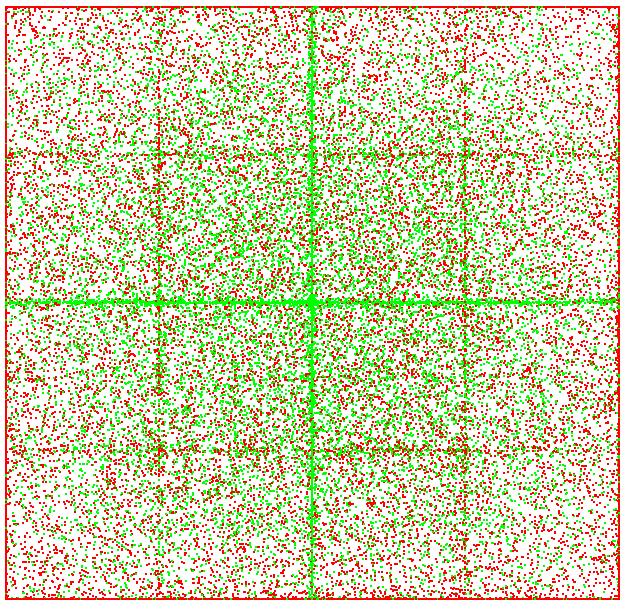
\includegraphics[width=1.0\textwidth, angle=0]{EMERGENT_PATTERN.png}
  	\caption{The emergent pattern used as criteria for qualitative comparison of implementations. Note the big green cross in the center and the smaller red crosses in each sub-sector. World-type is \textit{border} with 100.000 Agents where 25\% are Heroes.}
	\label{fig:EMERGENT_PATTERN}
\end{figure}


\subsection{Problem of RNG}
Have to behave EXACTLY The same: VERY difficult because of differing interfaces e.g. compare java to haskell RNGs.
Solution: create a deterministic RNG generating a number-stream starting from 1 and just counting up. The program should work also in this case, if not, something should be flawed!

Peer told me to implement a RNG-Trace: generate a list of 1000.0000 pre-calculated random-numbers in range of [0..1], store them in a file and read the trace in all implementations. Needs lots of implementation.

\subsection{Run-Time Complexity}
what if the number of agents grows? how does the run-time complexity of the simulation increases? Does it differ from implementation to implementation? The model is O(n) but is this true for the implementation?

\subsection{Simulation-Loops}
There are at least 2 parts to implementing a simulation: 1. implementing the logic of an agent and 2. implementing the iteration/recursion which drives the whole simulation

Classic \\
Yampa \\ TODO: use par to parallelize
Gloss \\
gloss provides means for simple simulation using simulate method. But: are all ABM systems like that?

\subsection{Agent-Representation}
Java: (immutable) Object
Haskell Classic: a struct
Haskell Yampa: a Signal-Function
Gloss: same as haskell classic
Akka: Actors

\subsection{EDSL}
simplify simulation into concise EDSL: distinguish between different kind if sims: continuous/discrete iteration on: fixed set, growing set, shrinking set, dynamic set. 

\section{Adding Spatiality}
When emulating the dynamics of the SIR model using an agent-based approach the question arises what we ultimately gain from doing so when we could have generated the dynamics much quicker and smoother using the SD approach. The difference is that the agent-based approach is a stochastic one and can thus also result in "degenerated" dynamics in which the disease dies out after a few steps or even can't spread from patient zero - in this case ABS is clearly a benefit as it allows to investigate \textit{alternative futures}, something not possible with SD in which the disease will never die out prematurely when there are non-zero infected agents. \\
Another advantage of ABS over SD is that agents can be heterogeneous and make use of spatial- and/or network-information defining the neighbourhood. We can thus simulate the spread of the disease throughout a population which is laid out on a 2D grid or one can investigate spreading of the disease throughout a network of agents where some are vaccinated and others not. We provide already suitable environments to simulate these cases and show an example of spreading the disease on a 2D grid in Figure \ref{fig:sir_spatial}.  

\begin{figure*}
\begin{center}
	\begin{tabular}{c c}
		\begin{subfigure}[b]{0.4\textwidth}
			\centering
			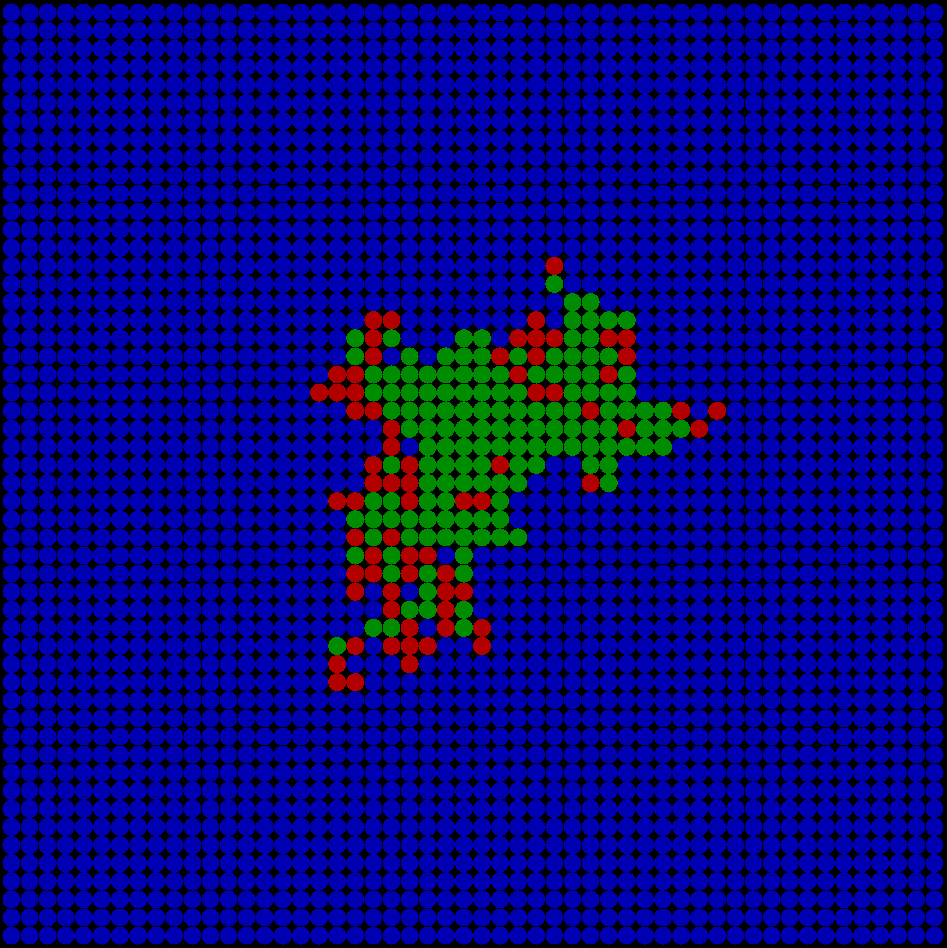
\includegraphics[width=.6\textwidth, angle=0]{./../shared/fig/spatial/SIR_spatial_52x52_92time.png}
			\caption{$t = 92$}
			\label{fig:sir_spatial_92}
		\end{subfigure}

		& 

		\begin{subfigure}[b]{0.4\textwidth}
			\centering
			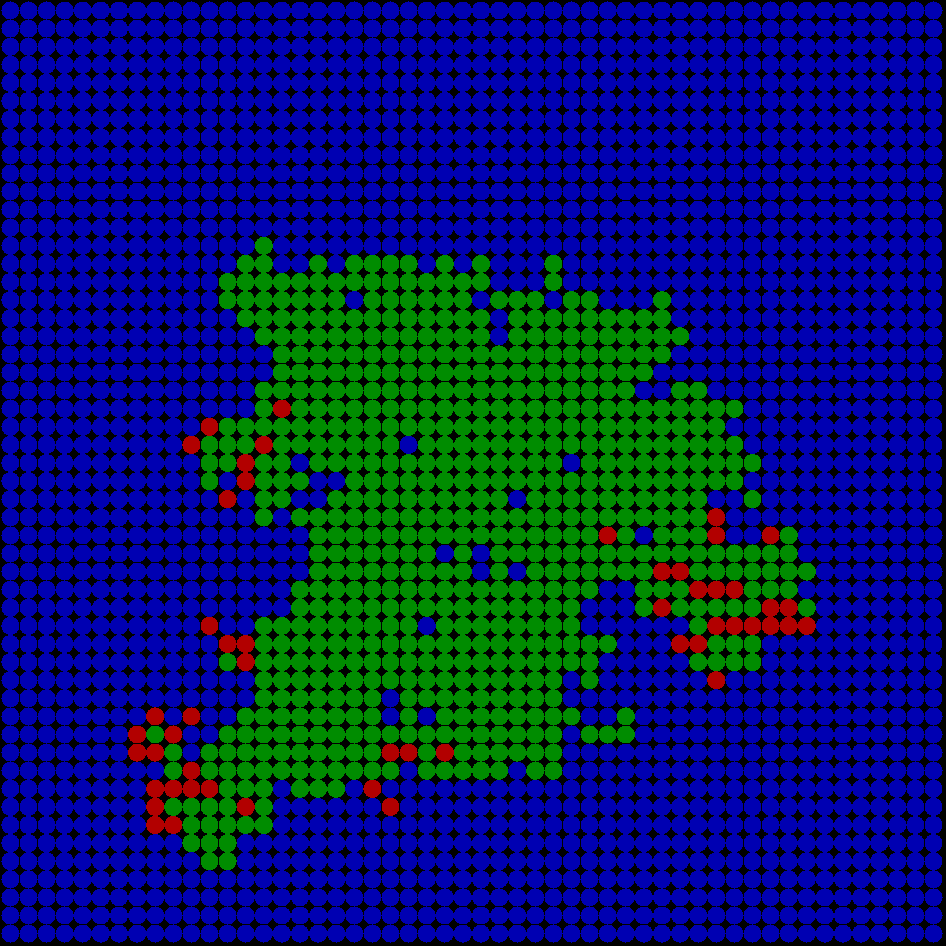
\includegraphics[width=.6\textwidth, angle=0]{./../shared/fig/spatial/SIR_spatial_52x52_200time.png}
			\caption{$t = 200$}
			\label{fig:sir_spatial_200}
		\end{subfigure}

		\\
		
		\begin{subfigure}[b]{0.4\textwidth}
			\centering
			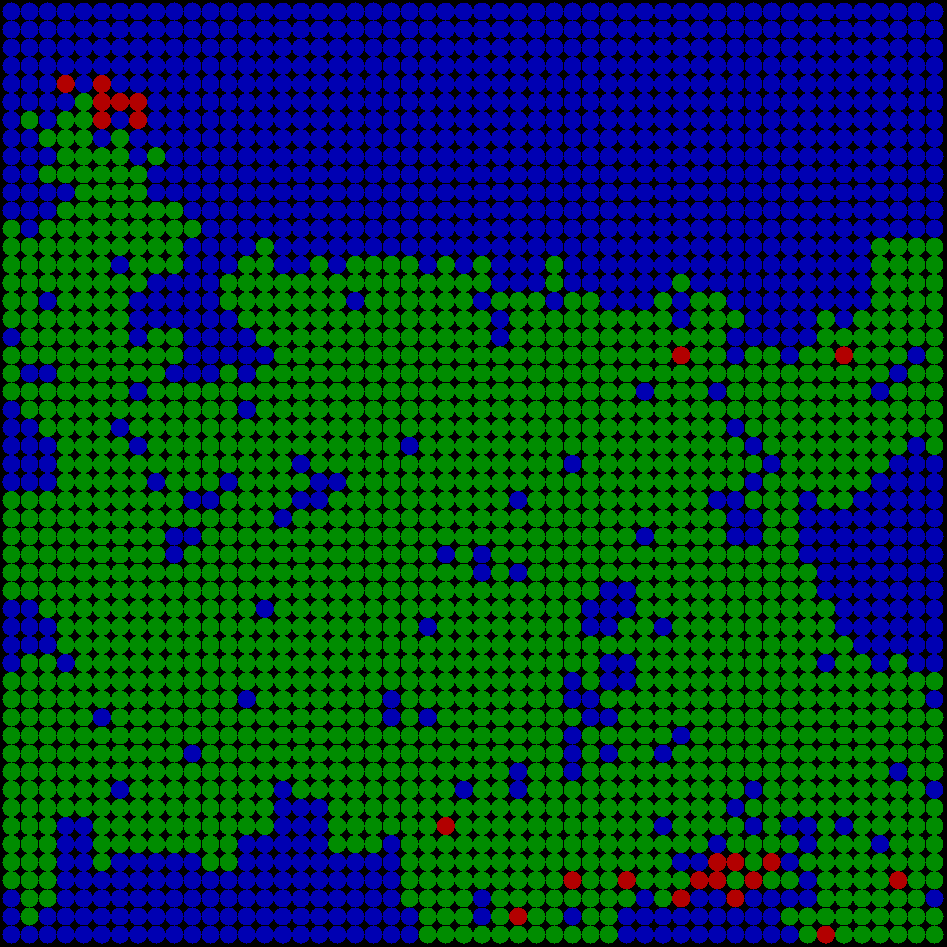
\includegraphics[width=.6\textwidth, angle=0]{./../shared/fig/spatial/SIR_spatial_52x52_440time.png}
			\caption{$t = 440$}
			\label{fig:sir_spatial_440}
		\end{subfigure}
		
		& 
		
		\begin{subfigure}[b]{0.4\textwidth}
			\centering
			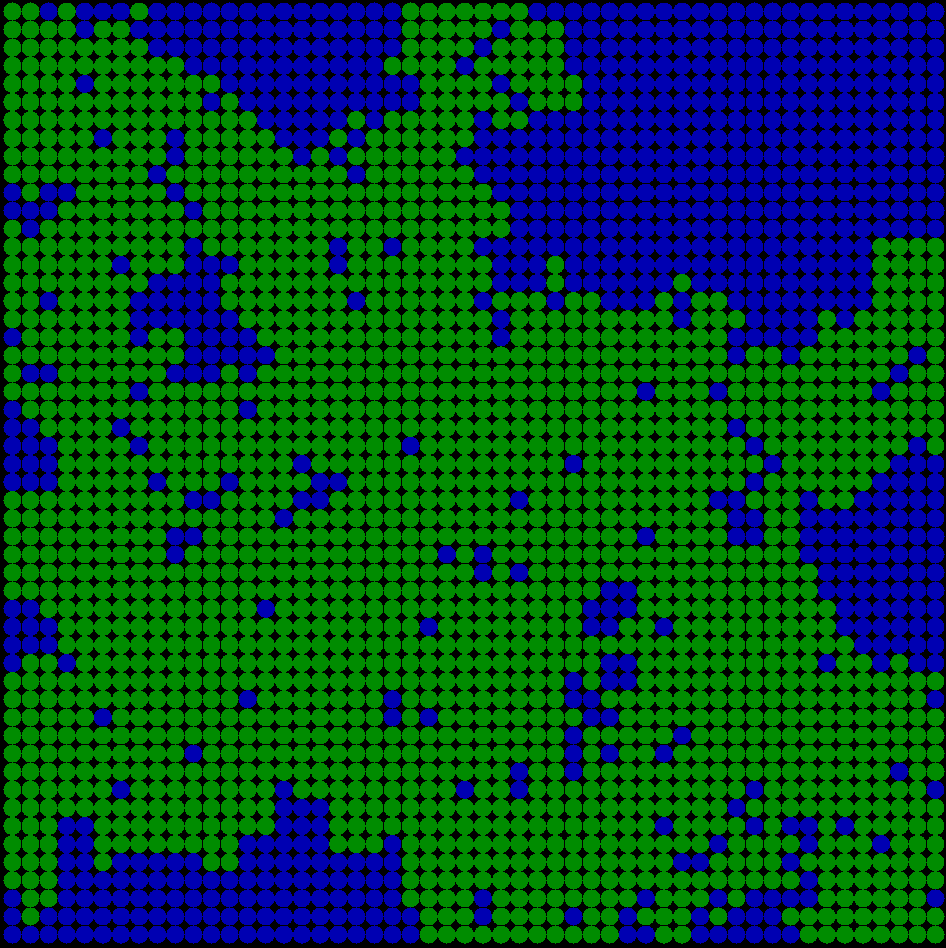
\includegraphics[width=.6\textwidth, angle=0]{./../shared/fig/spatial/SIR_spatial_52x52_873time.png}
			\caption{$t = 873$}
			\label{fig:sir_spatial_873}
		\end{subfigure}
	\end{tabular}
	
	\caption{Simulating SIR on a 52x52 grid with Moore neighbourhood using $\Delta t = 1$. Blue are susceptible, red are infected, green are recovered. The green areas act as protection as infected cannot cross the recovered border: this is particularly visible in the lower right corner of \ref{fig:sir_spatial_440} where the disease has been contained in the blue island and has no means to escape. It may seem that the few remaining infected agents in the top left corner of \ref{fig:sir_spatial_440} will die out soon but still it needs more than the already running simulation time until the disease actually dies out with the last patient recovering at center top of \ref{fig:sir_spatial_873} at $t = 873$. The dynamics of this simulation run can be seen in Figure \ref{fig:sir_spatial_dynamics}.} 
	\label{fig:sir_spatial}
\end{center}
\end{figure*}

\begin{figure}
	\centering
	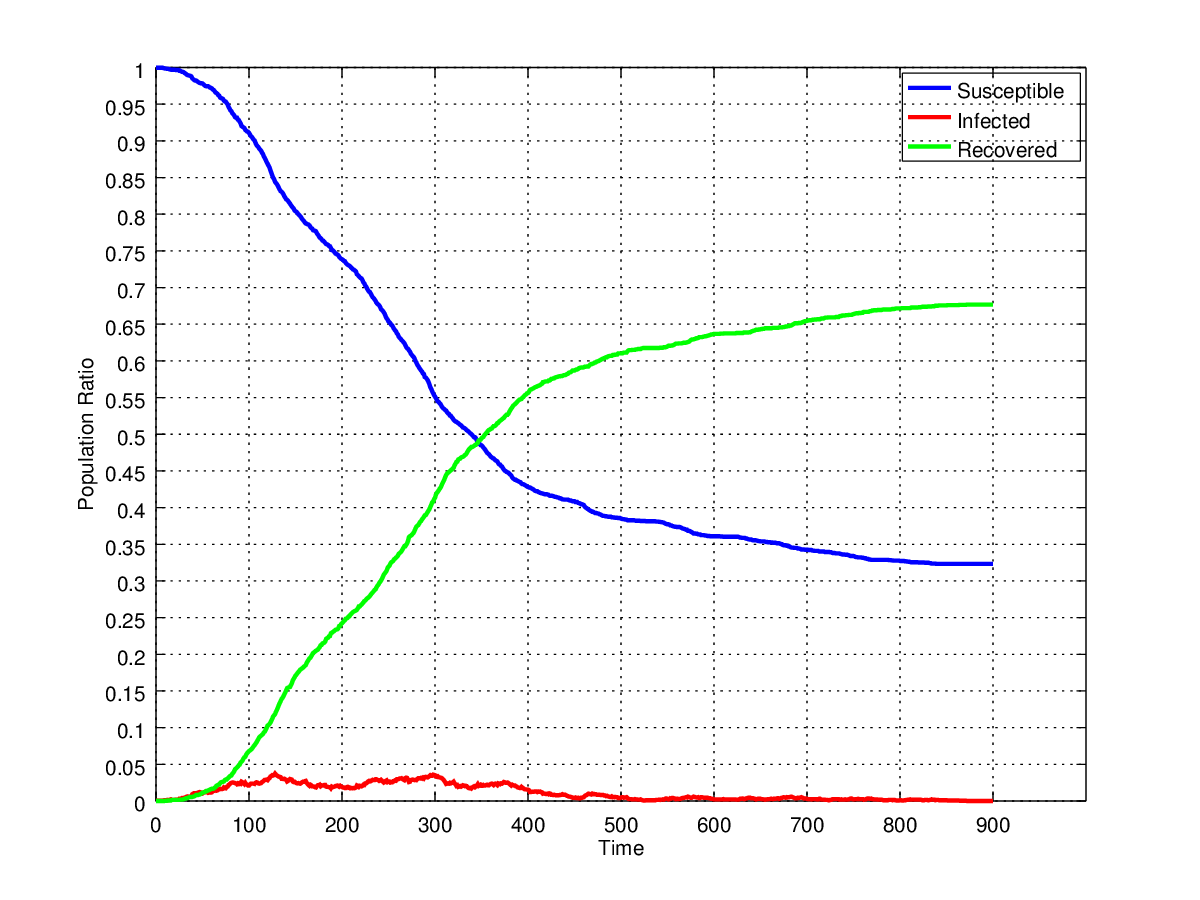
\includegraphics[width=.6\textwidth, angle=0]{./../shared/fig/spatial/SIR_spatial_dynamics_52x52_900time_1dt_parallel.png}
	\caption{Dynamics of the spatial SIR simulation from Figure \ref{fig:sir_spatial}.}
	\label{fig:sir_spatial_dynamics}
\end{figure}

Note that the dynamics of the spatial SIR simulation which are seen in Figure \ref{fig:sir_spatial_dynamics} look very different from the SD dynamics of Figure \ref{fig:sir_sd_dynamics}. This is due to a much more restricted neighbourhood which results in far fewer infected agents at a time and a lower number of recovered agents at the end of the epidemic, meaning that fewer agents got infected overall.

When using a 2D grid or network one needs to set them up in the initialization code so there is a little more work to do there but the implementation of the agents differ just in one single line, which is where the neighbourhood is picked - see line 100 of Appendix \ref{app:abs_code}. Instead of \textit{randomAgentIdMsgSource} one uses either \textit{randomNeighbourNodeMsgSource} in the case of a network or \textit{randomNeighbourCellMsgSource} in case of a 2D grid.

\section{Randomness and Super-Sampling}
TODO: maybe this subsection is unimportant

It is important to note that if we disable super-sampling and run the simulation for a given time \textit{t} but with two different $\Delta t$ we would end up with two different results, even if the $\Delta t$ are small enough to sample the time-dependent functions sufficiently. Also if we use super-sampling with $\Delta t = 1.0$ and create the exact same number of samples as when using no super-sampling but smaller $\Delta t$, then we also end up with different results.
The reason for this behaviour is that most of the time-dependent functions ultimately build upon drawing from random-distributions. With different $\Delta t$ we are generating a different number of random-samples, which would result in different random-number sequences which in turn ultimately leads to slightly different dynamics. When generating a plot of the dynamics this is not as visible, also this is the reason why one generates multiple replications, but this behaviour becomes strikingly apparent when simulating the SIR model on a 2D grid as can be seen in Figure \ref{fig:sir_abs_timeDeltas_randomness}.

\begin{figure*}
\begin{center}
	\begin{tabular}{c c}
		\begin{subfigure}[b]{0.4\textwidth}
			\centering
			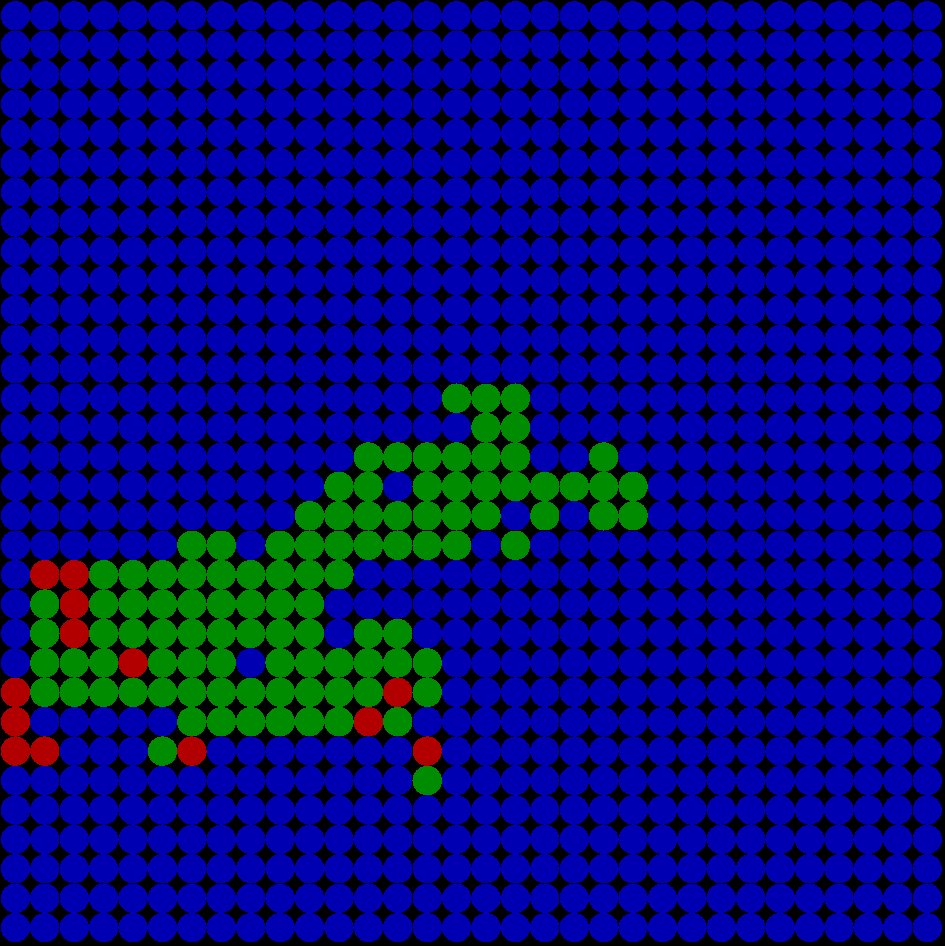
\includegraphics[width=.7\textwidth, angle=0]{./shared/fig/randomness/SIR_32x32_200time_01delta_noSS.png}
			\caption{$\Delta t = 0.1$, no super-sampling}
			\label{fig:sir_abs_timeDeltas_randomness_dt01}
		\end{subfigure}
	
		& 
		
		\begin{subfigure}[b]{0.4\textwidth}
			\centering
			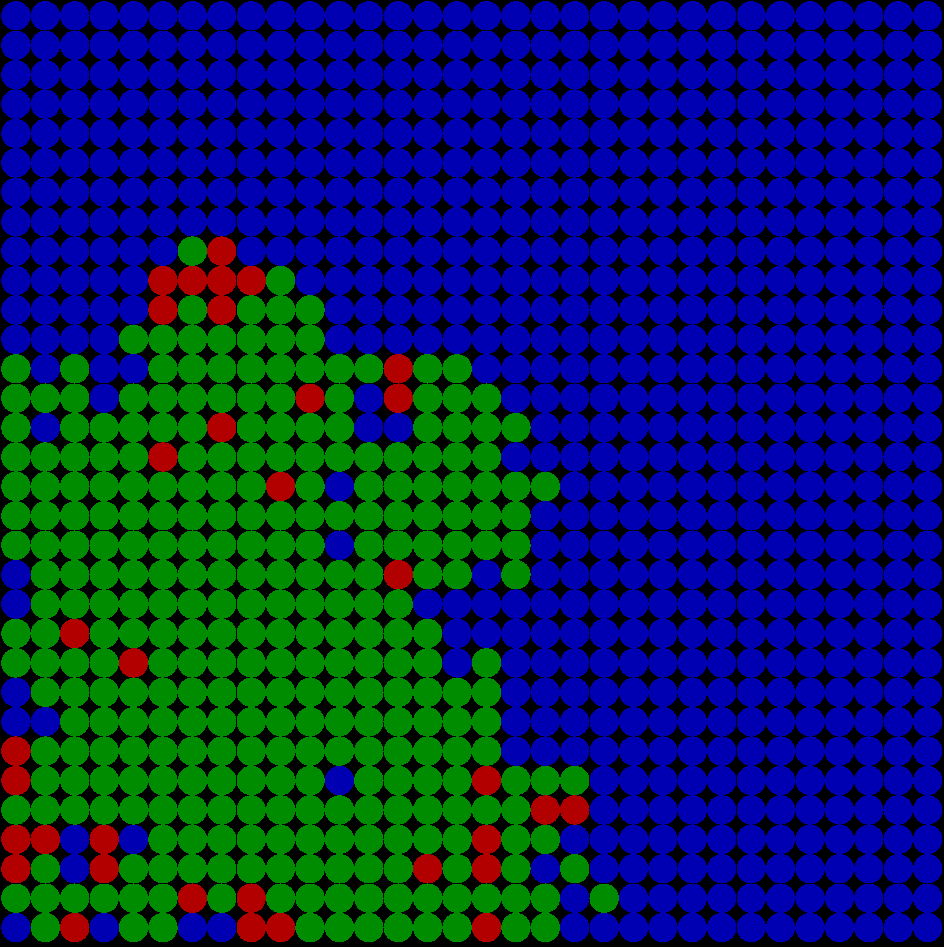
\includegraphics[width=.7\textwidth, angle=0]{./shared/fig/randomness/SIR_32x32_200time_001delta_noSS.png}
			\caption{$\Delta t = 0.01$, no super-sampling}
			\label{fig:sir_abs_timeDeltas_randomness_dt001}
		\end{subfigure}
		
		\\

		\begin{subfigure}[b]{0.4\textwidth}
			\centering
			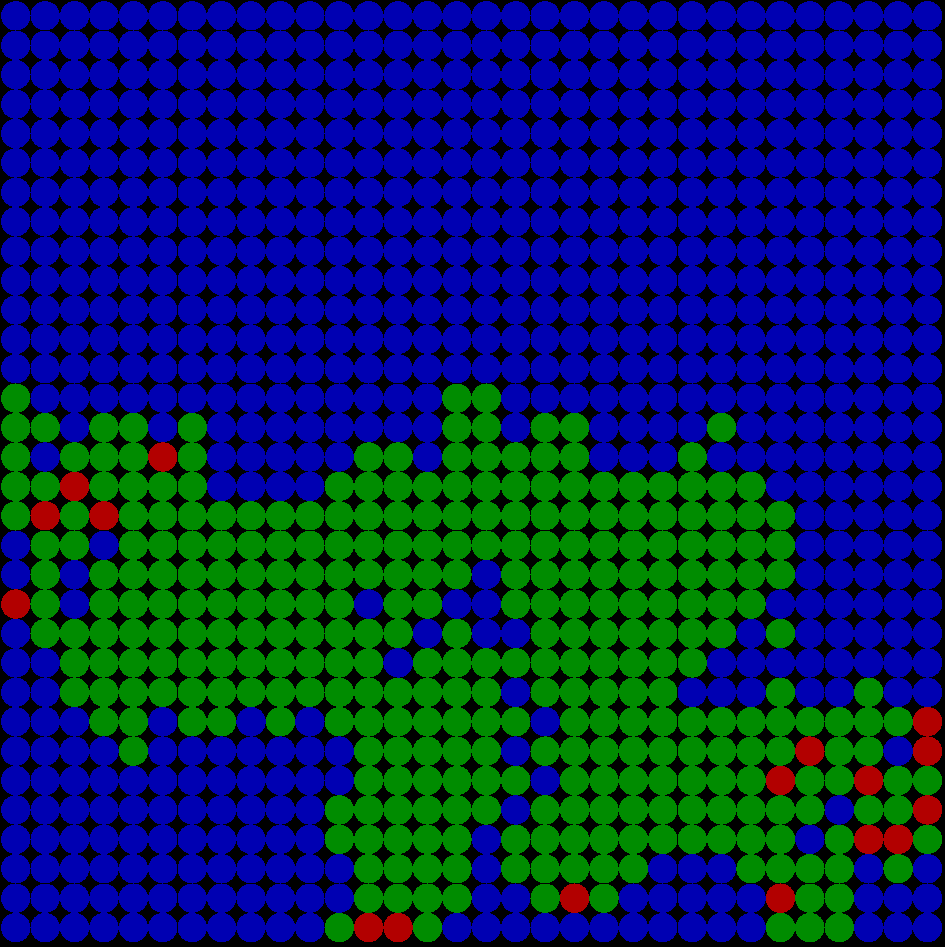
\includegraphics[width=.7\textwidth, angle=0]{./shared/fig/randomness/SIR_32x32_200time_10delta_ss10.png}
			\caption{$\Delta t = 1.0$ with 10 super-samples}
			\label{fig:sir_abs_timeDeltas_randomness_dt10_ss10}
		\end{subfigure}
		
		&
		
		\begin{subfigure}[b]{0.4\textwidth}
			\centering
			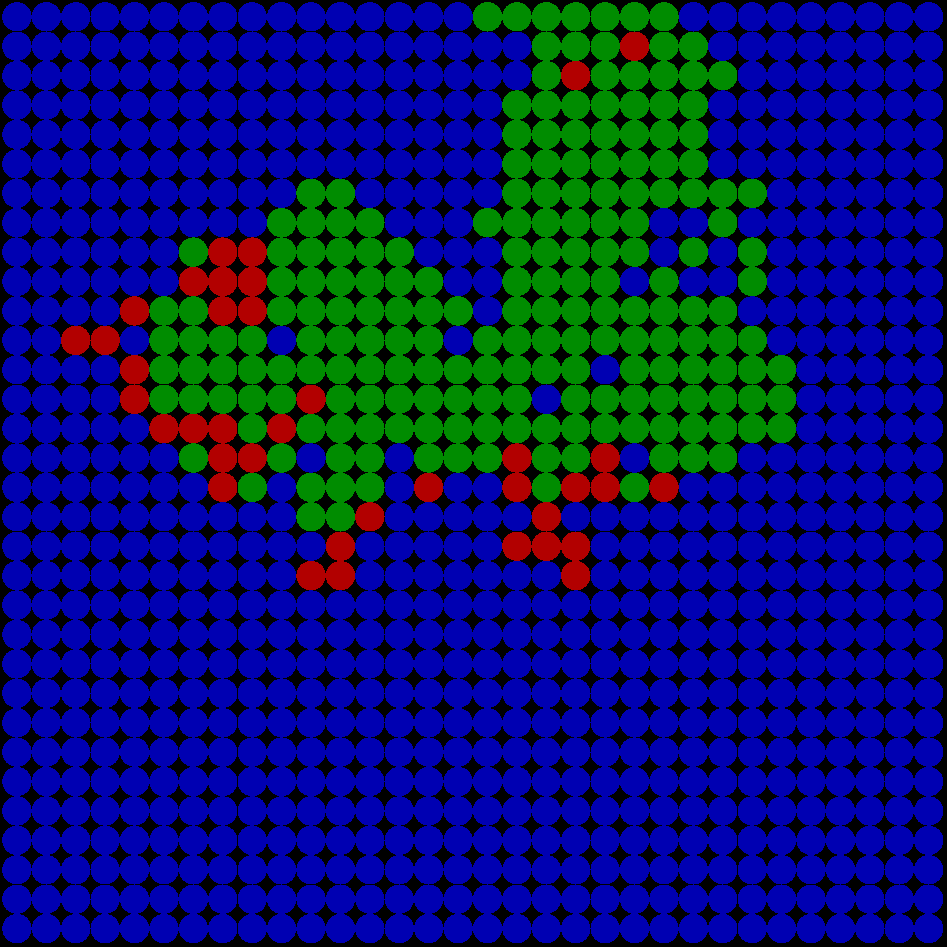
\includegraphics[width=.7\textwidth, angle=0]{./shared/fig/randomness/SIR_32x32_200time_10delta_ss100.png}
			\caption{$\Delta t = 1.0$ with 100 super-samples}
			\label{fig:sir_abs_timeDeltas_randomness_dt10_ss100}
		\end{subfigure}
	\end{tabular}
	
	\caption{Comparing results on 32x32 grid after $t = 200$ but with different $\Delta t$ and different number of super-samples.}
	\label{fig:sir_abs_timeDeltas_randomness}
\end{center}
\end{figure*}

\section{Agents as Signals}
Due to the underlying nature and motivation of FRP and Yampa, agents can be seen as signals which are generated and consumed by a signal-function which is the behaviour of an agent.  If an agent does not change, the output-signal should be constant amd if the agent changes e.g. by sending a message, changing its state,... the output-signal should change as well. A dead agent then should have no signal at all.
The question is if the agents of our agent-based SIR implementation are true signals: do the dynamics stay constant when we sample the system with $\Delta t = 0$? We hypothesize that our agents are true signals, thus they should not change when time does not change because they are completely time-dependent and rely completely on time-semantics. When actually running the simulation with $\Delta t = 0$ one gets the results as seen in Figure \ref{fig:sir_abs_zero_dt}.

\begin{figure*}
\begin{center}
	\begin{tabular}{c c}
		\begin{subfigure}[b]{0.5\textwidth}
			\centering
			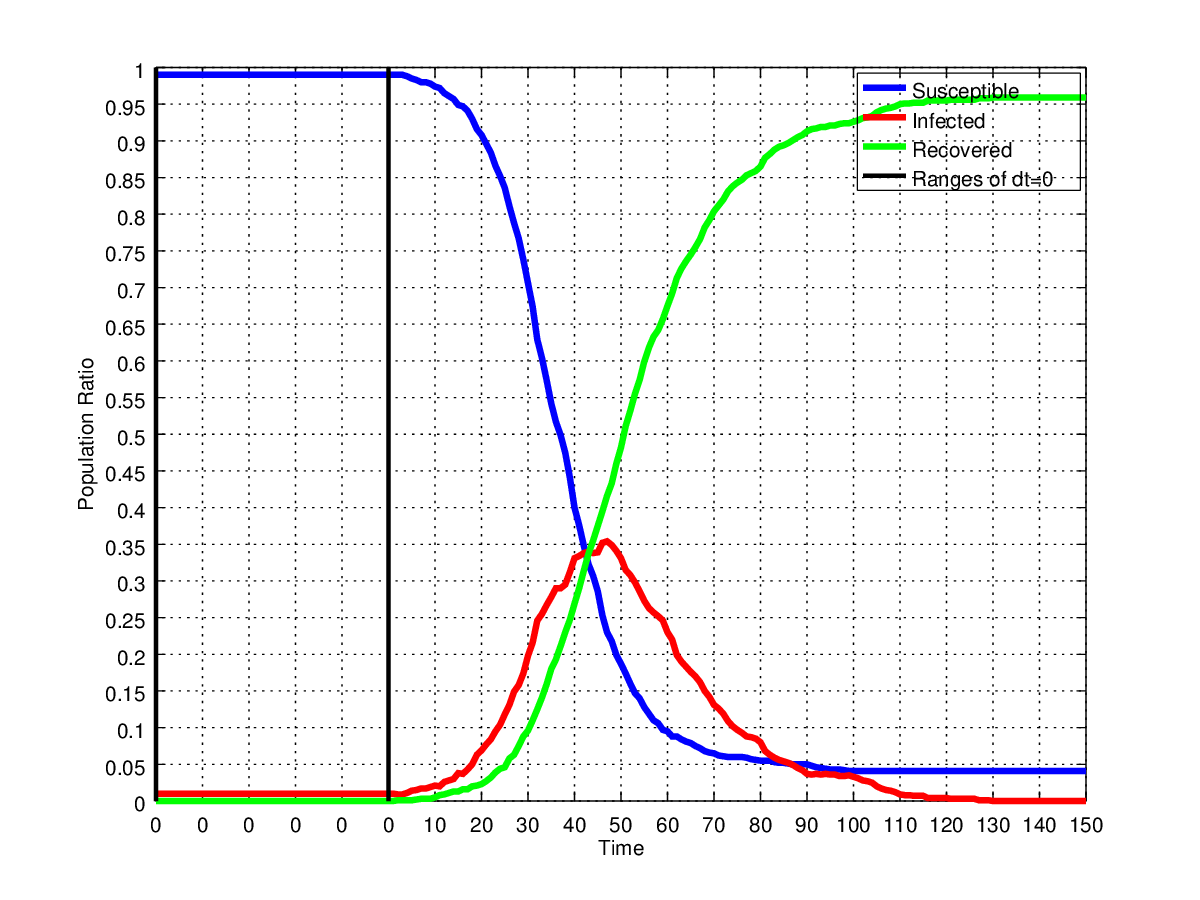
\includegraphics[width=.8\textwidth, angle=0]{./../shared/fig/dtzero/SIR_ABS_zeroDt_start.png}
			\caption{$\Delta t = 0$ from step 0 to 50.}
			\label{fig:sd_plot_10dt}
		\end{subfigure}
	
		& 
		
		\begin{subfigure}[b]{0.5\textwidth}
			\centering
			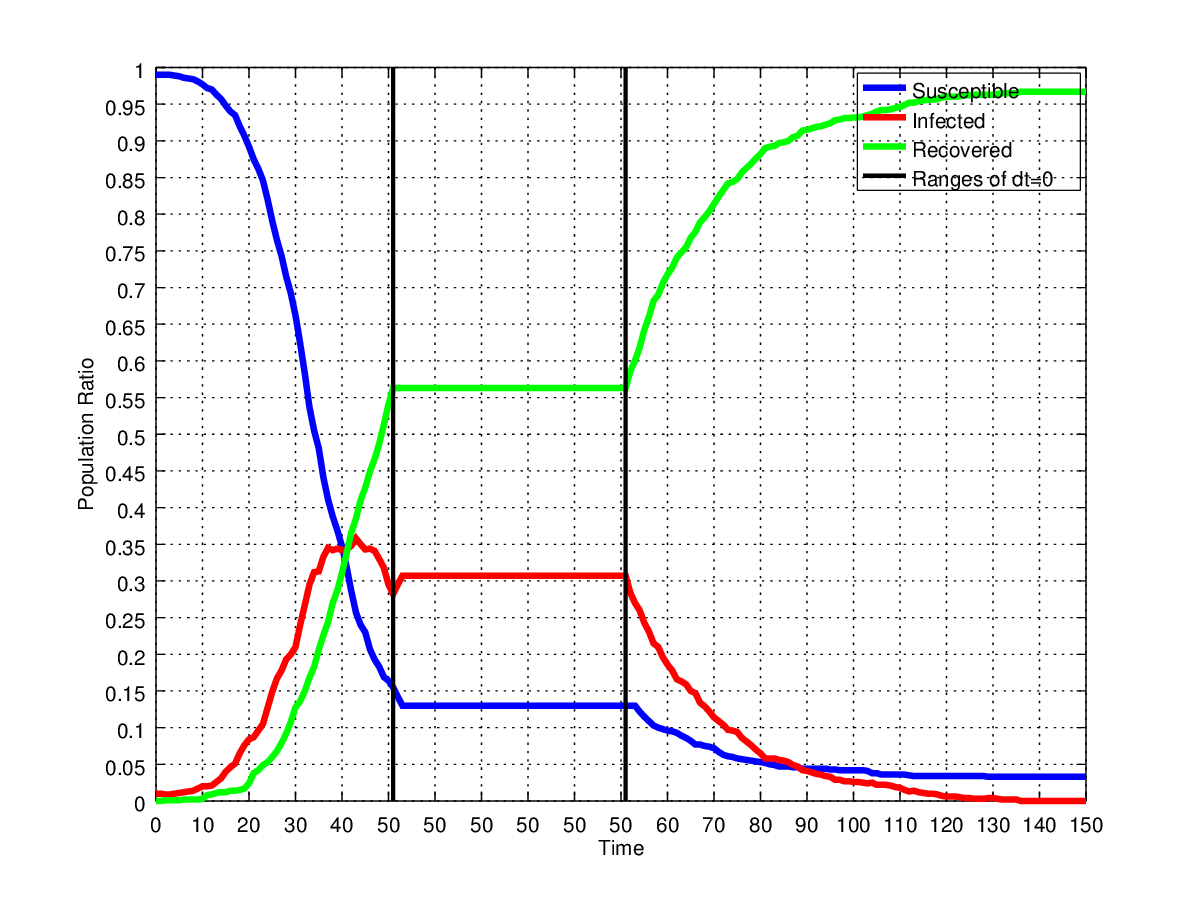
\includegraphics[width=.8\textwidth, angle=0]{./../shared/fig/dtzero/SIR_ABS_zeroDt_mid.png}
			\caption{$\Delta t = 0$ from step 51 to 101.}
			\label{fig:sd_plot_0.01dt}
		\end{subfigure}
	\end{tabular}
	
	\caption{Dynamics of agent-based SIR implementation of 1,000 agents running with $\Delta t = 1$ with ranges of $\Delta t = 0$ marked with two vertical black lines.}
	\label{fig:sir_abs_zero_dt}
\end{center}
\end{figure*}

As can be seen  the dynamics are becoming constant \textit{but} with a minor delay: infected increases a bit while susceptible decreases as can be seen in Figure \ref{fig:sir_abs_zero_dt_zoom}. This is due to the delay of message delivery which takes one $\Delta t$, independent of its value - messages are also delivered when $\Delta t = 0$. Only message-generating functions, which depend on non-zero $\Delta t$ to generate messages, will then stop generating messages. Reactive functions which act on incoming messages can still create change as they do not rely on time-semantics but just on the discrete event of a message arrival - which is the case in the transition from susceptible to infected.

\begin{figure}
	\centering
	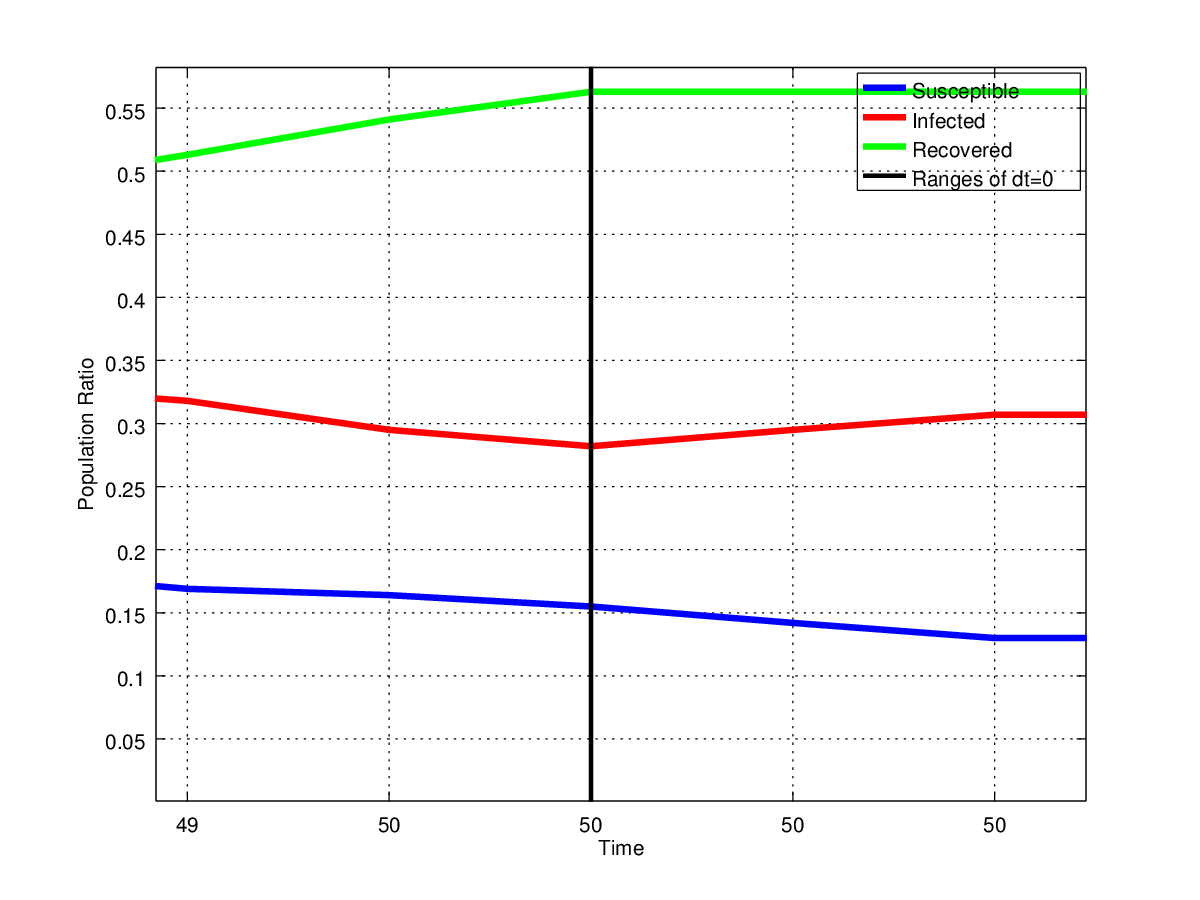
\includegraphics[width=.4\textwidth, angle=0]{./../shared/fig/dtzero/SIR_ABS_zeroDt_mid_zoom.png}
	\caption{Zoom-in to step 51, marked with the black line from where on $\Delta t = 0$ for the next 50 steps. The recovered ratio stays constant but a few agents get infected even \textit{after} having switched to $\Delta t = 0$ which happens due to the message delivery lag. After all messages have been delivered, the signal stays constant until non-zero $\Delta t$ are turned on again.}
	\label{fig:sir_abs_zero_dt_zoom}
\end{figure}

Note that agents of models with no time-semantics won't exhibit this behaviour - the dynamics will change even in case of $\Delta t = 0$ as agents act on every update and don't care about $\Delta t$ and just assume that every update occurs after $\Delta t$ independent of the actual value of it. We implemented the function \textit{doRepeatedlyEvery} which allows to transform a time-agnostic agent-behaviour into one. It is built on Yampas \textit{repeatedly} function and has the following signature:

\begin{minted}[fontsize=\footnotesize]{haskell}
doRepeatedlyEvery :: Time -> AgentBehaviour -> AgentBehaviour
\end{minted}

This function takes a time interval and an agent behaviour signal-function and returns a new agent behaviour signal-function which runs the argument signal-function every time-interval. Note that this function is subject to sampling issues. When the time-interval is very small one needs to run the simulation with a $\Delta t \leq Time$ otherwise the dynamics would show delayed activation of the agent behaviour.

\section{Discussion}
Although there are similarities to the work of \cite{botta_time_2010} (the use of messages and the problem of when to advance time in models with arbitrary number synchronised agent-interactions), we approach our agents differently. First in our approach an agent is only a single MSF and thus can not be directly queried for its internal state / its id or outgoing messages, instead of taking a list of messages, our agents take a single event/message and can produce an arbitrary number of outgoing messages together with an observable state - note that this would allow to query the agent for its id and its state as well by simply sending a corresponding message to the agents MSF and requiring the agent to implement message handling for it. Also the state of our agents is \textit{completely} localised and there is no means of accessing the state from outside the agent, they are thus "fully encapsulated agents" \cite{botta_time_2010}. Note that the authors of \cite{botta_time_2010} define their agents with a polymorphic agent-state type \textit{s}, which implies that without knowledge of the specific type of \textit{s} there would be no way of accessing the state, rendering it in fact also fully encapsulated. The problem of advancing time in our approach is solved not exactly the same but conceptually it is the same: after sending a tick message to each agent (in random order), we process all agents until they are idle: there are no more enqueued messages / events in the queue.

our eventdriven approach makes heavy use of 2 state monads, thus one might ask what the benefits are, after all we seem to fall back into stateful, imperative style programming. we agree that our approach is just one way of implementing abs in fp but we think we have come a long way thus making our approach quite valuable even if there might be other approaches like shallow EDSLs. on the other hand even our stateful programming is highly restricted to only those 2 local datatypes which makes it much more manageable than unrestricted data mutation

quote carmack (\url{http://www.gamasutra.com/view/news/169296/Indepth_Functional_programming_in_C.php}): the main difficulty as a developer in software programming is to keep track of the states a program can be in and reason about them and their Validity

TODO: report LoC and compare it with other implementations we found on the internet

\section{Related Research}
Already noted in the Introduction, \cite{huberman_evolutionary_1993} where the first to discuss the differences update-strategies can make and introduced the terms of synchronous and asynchronous updates. They define to be synchronous as agents being updated in unison and asynchronous where one agent is updated and the others are held constant.

\medskip

\cite{a_framework_2008} give an approach for ABS on GPUs which is a very different approach to updating and iterating agents in ABS. They discuss execution order at length, highlight the problem of inducing a specific execution-order in a model which is problematic for parallel execution and give solutions how to circumvent these shortcomings. Although we haven't mapped our ideas to GPUs we explicitly include an approach for data-parallelism which, we hypothesize, can be utilized to roughly map their approach onto our terminology. 
	
\medskip
	
\cite{botta_time_2010} sketch a minimal ABS implementation in Haskell which is very similar in the basic structure of ours. This proves that our approach seems to be a very natural one to apply to Haskell. Their focus is primarily on economic simulations and instead of iterating a simulation with a global time, their focus is on how to synchronize agents which have internal, local transition times. Although their work uses Haskell as well, our focus is very different from theirs and approaches ABS in a more general and comprehensive way.

\medskip

\cite{dawson_opening_2014} describe basic inner workings of ABS environments and compare their implementation in C++ to the existing ABS environment AnyLogic which is programmed in Java. They explicitly mention asynchronous and synchronous time-models and compare them in theory but unfortunately couldn't report the results of asynchronous updates due to limited space. They interpret asynchronous time-models to be the ones in which an agent acts at random time intervals and synchronous time-models where agents are updated all in same time intervals.

\medskip

\cite{yuxuan_agent-based_2016} presents in his Master-Thesis a comprehensive discussion on how to implement an ABS for state-charts in Java and also mentions synchronous and asynchronous time-models. He identifies the asynchronous time-model to be one in which updates are triggered by the exchange of messages and the synchronous ones which trigger changes immediately without the indirection of messages.

\medskip

We observe that there seems to be a variety of meanings attributed to the terminology of asynchronous and synchronous updates but the very semantic and technical details are unclear and not described very precisely. In the next section we will address this issue by presenting the basic background and propose properties for a new terminology from which we can derive common update-strategies.

\section{Conclusion and further research}

So far we only looked at recursive simulation in a simulation with a strictly sequential update-strategy where agents are updated in sequence after each other as defined in TODO: cite my Art-Of-Iteration Paper. We leave the question of how Meta-ABS would apply to the parallel update-strategy and whether it is reasonable to extend it to that strategy or not for further research.

Research Questions
\begin{enumerate}
	\item How does deep regression influence the dynamics of a system? Hypothesis: TODO
	\item How do the dynamics of a system change when using perfect information or learning local information? Hypothesis: TODO
	\item Is a hidden markov model suitable for the local learning? Hypothesis: TODO
	\item How can MetaABS best be implemented? Hypothesis: implementing a MetaABS EDSL in a pure functional language like Haskell, should be best suited due to its inherent recursive, declarative nature, which should allow a direct mapping of features of this paradigm to the specification of the meta-model
\end{enumerate}

Problems
\begin{itemize}
	\item Definition of a recursive, declarative description of the Model.
	\item Perfect information about other agents is not realistic and runs counter to agent-based simulation (especially in social sciences) thus an Agent needs to be able to have local, noisy representations of the other agents.
	\item Local representation of other agents could be captured by Hidden Markov Models: observe what other agents do but have hidden interpretation of their internal state - these internal state-representations can be different between the local and the global version whereas the agent learns to represent the global version as best as possible locally.
	\item Infinite regress is theoretically possible but not on computers, we need to terminate at some point
\end{itemize}

\section*{Acknowledgments}
The authors would like to thank I. Perez, H. Nilsson, J. Greensmith, T. Schwarz and H. Vollbrecht for constructive comments and valuable discussions.

\bibliographystyle{../../papers/templates/IEEEtran/bibtex/IEEEtran}
\bibliography{../../../papers/references/phdReferences.bib}

\appendices

\newpage
\section{Full code of the agent-based SIR implementation}
\label{app:abs_code}

\begin{minted}[fontsize=\footnotesize, linenos]{haskell}
data SIRState = Susceptible | Infected | Recovered deriving (Eq)
data SIRMsg = Contact SIRState deriving (Eq)

type SIRAgentState = SIRState

type SIREnvironment = [AgentId]

type SIRAgentDef = AgentDef SIRAgentState SIRMsg SIREnvironment
type SIRAgentBehaviour = AgentBehaviour SIRAgentState SIRMsg SIREnvironment
type SIRAgentBehaviourReadEnv = ReactiveBehaviourReadEnv SIRAgentState SIRMsg SIREnvironment
type SIRAgentBehaviourIgnoreEnv = ReactiveBehaviourIgnoreEnv SIRAgentState SIRMsg SIREnvironment
type SIRAgentIn = AgentIn SIRAgentState SIRMsg SIREnvironment
type SIRAgentOut = AgentOut SIRAgentState SIRMsg SIREnvironment
type SIRAgentObservable = AgentObservable SIRAgentState

type SIREventSource = EventSource SIRAgentState SIRMsg SIREnvironment

-------------------------------------------------------------------------------
infectivity :: Double
infectivity = 0.05

contactRate :: Double
contactRate = 5

illnessDuration :: Double
illnessDuration = 15

contactSS :: Int
contactSS = 20

illnessTimeoutSS :: Int
illnessTimeoutSS = 2

-------------------------------------------------------------------------------
createSIRNumInfected :: Int -> Int -> IO ([SIRAgentDef], SIREnvironment)
createSIRNumInfected agentCount numInfected = do
    let agentIds = [0 .. (agentCount-1)]
    let infectedIds = take numInfected agentIds
    let susceptibleIds = drop numInfected agentIds

    adefsSusceptible <- mapM (sirAgent Susceptible) susceptibleIds
    adefsInfected <- mapM (sirAgent Infected) infectedIds

    return (adefsSusceptible ++ adefsInfected, agentIds)

sirAgent :: SIRState -> AgentId -> IO SIRAgentDef
sirAgent initS aid = do
    rng <- newStdGen
    let beh = sirAgentBehaviour rng initS
    let adef = AgentDef { 
          adId = aid
        , adState = initS
        , adBeh = beh
        , adInitMessages = NoEvent
        , adConversation = Nothing
        , adRng = rng 
        }

    return adef
   
-------------------------------------------------------------------------------
-- UTILITIES
gotInfected :: SIRAgentIn -> Rand StdGen Bool
gotInfected ain = onMessageM gotInfectedAux ain False
  where
    gotInfectedAux :: Bool -> AgentMessage SIRMsg -> Rand StdGen Bool
    gotInfectedAux False (_, Contact Infected) = randomBoolM infectivity
    gotInfectedAux x _ = return x



respondToContactWith :: SIRState -> SIRAgentIn -> SIRAgentOut -> SIRAgentOut
respondToContactWith state ain ao = onMessage respondToContactWithAux ain ao
  where
    respondToContactWithAux :: AgentMessage SIRMsg -> SIRAgentOut -> SIRAgentOut
    respondToContactWithAux (senderId, Contact _) ao = sendMessage (senderId, Contact state) ao

-- SUSCEPTIBLE
sirAgentSuceptible :: RandomGen g => g -> SIRAgentBehaviour
sirAgentSuceptible g = 
	transitionOnEvent 
		sirAgentInfectedEvent 
		(readEnv $ sirAgentSusceptibleBehaviour g) 
		(sirAgentInfected g)

sirAgentInfectedEvent :: SIREventSource
sirAgentInfectedEvent = proc (ain, ao) -> do
    let (isInfected, ao') = agentRandom (gotInfected ain) ao 
    infectionEvent <- edge -< isInfected
    returnA -< (ao', infectionEvent)

sirAgentSusceptibleBehaviour :: RandomGen g => g -> SIRAgentBehaviourReadEnv
sirAgentSusceptibleBehaviour g = proc (ain, e) -> do
    ao' <- doOnce (setAgentState Susceptible) -< agentOutFromIn ain
    returnA -< sendMessageOccasionallySrcSS 
    			g
    			(1 / contactRate)
    			contactSS
    			(randomAgentIdMsgSource (Contact Susceptible) True) -< (ao', e)

-- INFECTED
sirAgentInfected :: RandomGen g => g -> SIRAgentBehaviour
sirAgentInfected g = 
	transitionAfterExpSS 
		g 
		illnessDuration 
		illnessTimeoutSS 
		(ignoreEnv $ sirAgentInfectedBehaviour g) 
		sirAgentRecovered

sirAgentInfectedBehaviour :: RandomGen g => g -> SIRAgentBehaviourIgnoreEnv
sirAgentInfectedBehaviour g = proc ain -> do
    ao' <- doOnce (setAgentState Infected) -< agentOutFromIn ain
    returnA -< respondToContactWith Infected ain ao'

-- RECOVERED
sirAgentRecovered :: SIRAgentBehaviour
sirAgentRecovered = doOnceR $ setAgentStateR Recovered

-- INITIAL CASES
sirAgentBehaviour :: RandomGen g => g -> SIRState -> SIRAgentBehaviour
sirAgentBehaviour g Susceptible = sirAgentSuceptible g
sirAgentBehaviour g Infected = sirAgentInfected g
sirAgentBehaviour _ Recovered = sirAgentRecovered

-------------------------------------------------------------------------------
runSIR :: IO ()
runSIR = do
    -- parallel strategy, no updating/folding of environment, no shuffling, rng-seed of 42
    params <- initSimulation Parallel Nothing Nothing False (Just 42)
    (initAdefs, initEnv) <- createSIRNumInfected agentCount numInfected
    let dynamics = simulateAggregateTime initAdefs initEnv params dt t aggregate
    print dynamics
	
aggregate :: (Time, [SIRAgentObservable], SIREnvironment) -> (Time, Double, Double, Double)
aggregate (t, aobs, _) = (t, susceptibleCount, infectedCount, recoveredCount)
  where
    susceptibleCount = fromIntegral $ length $ filter ((Susceptible==) . snd) aobs
    infectedCount = fromIntegral $ length $ filter ((Infected==) . snd) aobs
    recoveredCount = fromIntegral $ length $ filter ((Recovered==) . snd) aobs
\end{minted}

\end{document}

\section{Conclusion and further research}

So far we only looked at recursive simulation in a simulation with a strictly sequential update-strategy where agents are updated in sequence after each other as defined in TODO: cite my Art-Of-Iteration Paper. We leave the question of how Meta-ABS would apply to the parallel update-strategy and whether it is reasonable to extend it to that strategy or not for further research.

Research Questions
\begin{enumerate}
	\item How does deep regression influence the dynamics of a system? Hypothesis: TODO
	\item How do the dynamics of a system change when using perfect information or learning local information? Hypothesis: TODO
	\item Is a hidden markov model suitable for the local learning? Hypothesis: TODO
	\item How can MetaABS best be implemented? Hypothesis: implementing a MetaABS EDSL in a pure functional language like Haskell, should be best suited due to its inherent recursive, declarative nature, which should allow a direct mapping of features of this paradigm to the specification of the meta-model
\end{enumerate}

Problems
\begin{itemize}
	\item Definition of a recursive, declarative description of the Model.
	\item Perfect information about other agents is not realistic and runs counter to agent-based simulation (especially in social sciences) thus an Agent needs to be able to have local, noisy representations of the other agents.
	\item Local representation of other agents could be captured by Hidden Markov Models: observe what other agents do but have hidden interpretation of their internal state - these internal state-representations can be different between the local and the global version whereas the agent learns to represent the global version as best as possible locally.
	\item Infinite regress is theoretically possible but not on computers, we need to terminate at some point
\end{itemize}

\bibliographystyle{acm}
\bibliography{../../references/phdReferences.bib}

\end{document}


\section{Concurrency}
This section is a quite extensive one, due to the much complexer nature of the topic. In this chapter we focus on the use of Software Transactional Memory (STM) to implement concurrent ABS in Haskell. There exist mechanisms for traditional lock-based concurrency in Haskell as well, but even though due to Haskells type system and pure functional nature, we would still suffer similar problems, imperative solutions suffer. Thus we focus on the unique way Haskell implements and enables STM and show that it is indeed a very powerful abstraction to implement concurrent ABS. Note that STM is by now available in imperative oop languages as well, but we will show that it is only in Haskell with its type system where it really shines and can guarantee its semantics.


\chapter{Verification \& Correctness}
Testing of functional ABS paper
10\%

- correctness \& verification
	-> static type system eliminates a large number run-time bugs: if we decide to rule out IO then we can guarantee 


\chapter{Dependent Types}
%My work is all nice and good but it solves problems the ABS community and implementations never really had. My FRP/MSF approach is quite complex and can be equally difficult to get right. Even worse, the bugs were not primarily those I am solving with FP but the REAL problem in ABS is translating the model into code. Can FP help us here? Can my pure FP approach help here? expressing invariants in FP code? can we express them in types? 

The pure functional implementation techniques have a number of technical benefits but don't help as much in closing the gap between specification and implementation as one is used from functional programming in general. Therefore we take a step back and abstract from these highly complex implementation techniques and move towards dependent types. Follow \cite{botta_time_2010} and \cite{botta_functional_2011}.

Conceptually discuss how dependent types can be made of use in ABS without going into lot of technical detail because: 1. i didn't do enough research on it and 2. dependent types seem to be nearly out of focus of the thesis.

%Linear and Dependent Types with Idris 2: more general ideas / hints / research on how it is applicable to ABS

%dependent types in ABS paper, explore totality - equilibrium correspondence idea
%About 20\% finished.

\section{Discussion}
Although there are similarities to the work of \cite{botta_time_2010} (the use of messages and the problem of when to advance time in models with arbitrary number synchronised agent-interactions), we approach our agents differently. First in our approach an agent is only a single MSF and thus can not be directly queried for its internal state / its id or outgoing messages, instead of taking a list of messages, our agents take a single event/message and can produce an arbitrary number of outgoing messages together with an observable state - note that this would allow to query the agent for its id and its state as well by simply sending a corresponding message to the agents MSF and requiring the agent to implement message handling for it. Also the state of our agents is \textit{completely} localised and there is no means of accessing the state from outside the agent, they are thus "fully encapsulated agents" \cite{botta_time_2010}. Note that the authors of \cite{botta_time_2010} define their agents with a polymorphic agent-state type \textit{s}, which implies that without knowledge of the specific type of \textit{s} there would be no way of accessing the state, rendering it in fact also fully encapsulated. The problem of advancing time in our approach is solved not exactly the same but conceptually it is the same: after sending a tick message to each agent (in random order), we process all agents until they are idle: there are no more enqueued messages / events in the queue.

our eventdriven approach makes heavy use of 2 state monads, thus one might ask what the benefits are, after all we seem to fall back into stateful, imperative style programming. we agree that our approach is just one way of implementing abs in fp but we think we have come a long way thus making our approach quite valuable even if there might be other approaches like shallow EDSLs. on the other hand even our stateful programming is highly restricted to only those 2 local datatypes which makes it much more manageable than unrestricted data mutation

quote carmack (\url{http://www.gamasutra.com/view/news/169296/Indepth_Functional_programming_in_C.php}): the main difficulty as a developer in software programming is to keep track of the states a program can be in and reason about them and their Validity

TODO: report LoC and compare it with other implementations we found on the internet

\chapter{Conclusions}
\label{chap:concl}

\section{Being Realistic}
It is of most importance to stress that we don't condemn the current state-of-the-art approach of object-oriented specification and implementation to ABS. The strength of object-oriented programming is surely that it can be seen as \textit{programming as modelling} and thus will be always an attractive approach to ABS. Also we are realists and know that there are more points to consider when selecting a set of methods for developing software for an ABS than robustness, verification and validation. Almost always the popularity of an existing language and which languages the implementer knows is the driving force behind which methods and languages to choose. This means that ABS will continue to be implemented in object-oriented programming languages and many perfectly well functioning models will be created by it in the future. Although they all suffer from the same issues mentioned in the introduction this doesn't matter as they are not of central importance to most of them.
Nonetheless we think our work is still essential and necessary as it may start a slow paradigm-shift and opens up the minds of the ABS community to a more functional and formal way of approaching and implementing agent-based models and simulations and recognizing the benefits one gets automatically from it by doing so.

\section{What we are not doing}
Because of this highly interdisciplinary topic we explicitly mention what we do not want to undertake in this PhD.
First we don't want to develop another language for formal agent-specification which needs to be compiled or used in some fancy tool - we want to put it directly into Haskell, building on the existing facilities.
Second, we are not developing a new economic theory about decentralized bilateral bartering, we take the existing theory and existing agent-based models and apply our methods to them.
Third, we don't want to use fancy statistics and number juggling for comparing validating and verifying models: we want structural comparison (category-theory).
Fourth, we do NOT want to do a direct comparison of object-orientation vs. functional in ABS, as we would get lost in an infinite amount of low-level technical details. We look at the benefits / drawbacks more on a conceptual level, applied to ABS.

\renewcommand\bibname{References}

\bibliographystyle{acm}
\bibliography{../references/phdReferences}

\begin{appendices}

\chapter{Pure Functional Epidemics}
\label{app:pfe}
Submission history:
\begin{enumerate}
	\item Submitted to Haskell Symposium 2018 on 30th March \\ REJECTED on 18th May
	\item Submitted to IFL 2018 on 25th May \\ NOTIFICATION PENDING until 20th July
\end{enumerate}

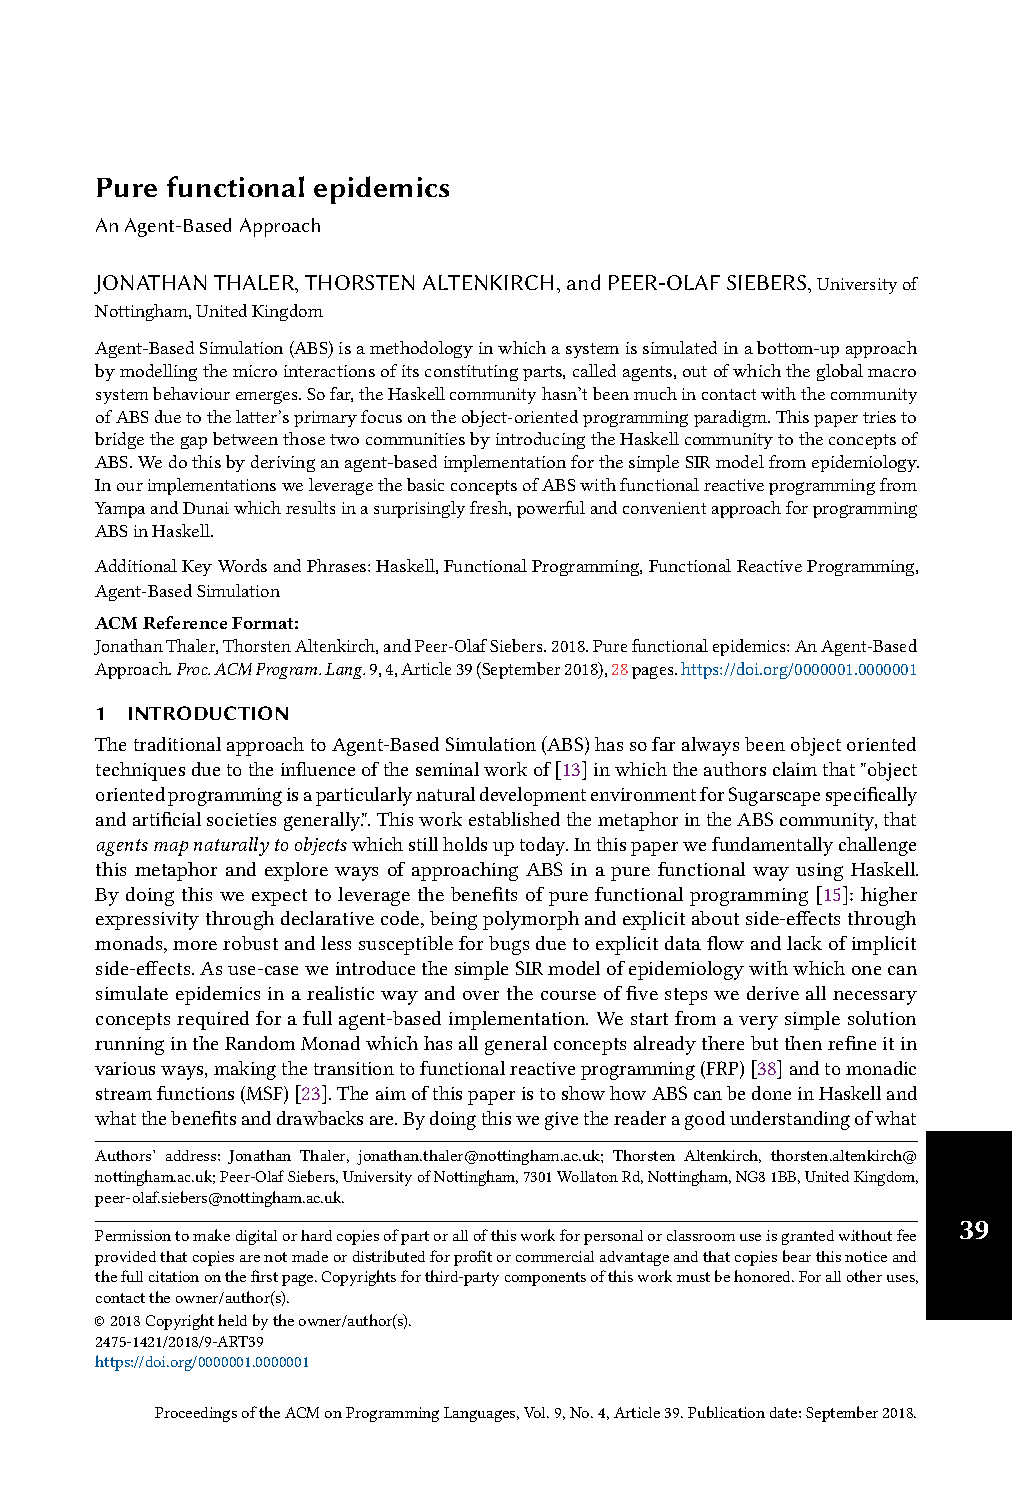
\includepdf[pages=-]{./pdf/pfe.pdf}

% NOTE: keep it out to the submission for the reviewers
%\chapter{Questions \& Answers}
\label{chap:qa}

TODO: update and adopt to 2nd year

In this chapter I give answers to anticipated questions and objections about my research direction and vision of doing pure functional ABS \footnote{They are not always posed in a dead-serious way but as it is a quite controversial topic - ABS should be done object-orientated after all huh? - I think it is appropriate. Also some objections were raised in exactly this way.}.

\paragraph{So you had this hypothesis, that pure functional programming and dependent types lead to simulation software which is more likely correct and is easier to verify and validate, right from the beginning?}
Not at all. I even had no deep knowledge of functional programming at the start of my PhD, I've just worked through the 1st edition of Grahams book "Programming in Haskell" and that's it. I had no clear understanding of purity, side-effects and Monads and I didn't know a bit about functional reactive programming. I knew that something like Dependent Types exist because Thorsten (2nd Supervisor) has sent me an email before the start of my PhD in which he pointed at Agda, so I started reading a bit about intuitionistic / constructivistic math, tried out a little bit of Agda but quickly gave up because it was way too far away (without really having mastered pure functional programming in Haskell, I believe it is nearly impossible / too difficult / makes no sense going into dependent types).
So in the beginning there was pure \textit{curiosity} about functional programming in combination with ABS because I knew nothing of FP at all and wanted to understand it (after getting bored by OO) and applying FP to ABS seemed so crazy (because everyone claims OO to be 'natural' for it) that it must be an extremely interesting challenge. I guess this is very often the case with research: there is 'just' curiosity in the beginning and then during the research process a hypothesis falls into place.


\chapter{Thesis Structure}
\label{app:thesis_struct}

TODO: find the story of my PhD thesis and connect it to my publication plan. 
TODO: story e.g. "We need functional programming to reduce the potential sources of bugs and introducing bugs harder, resulting in software which is more likely to be correct. Additionally by using dependent types we can narrow the gap between model specification and implementation even further, resulting in software which is even more likely to be correct. Further, additional benefits fall into place: purity leads to guaranteed reproducibility at compile-time, software transactional memory can be utilised to scale up to massively parallel and we have property-based testing at hand which puts the focus on specification testing rather than testing operational details".

This appendix gives a first draft of the structure outline of the thesis which I plan on start writing in April 2019. I aim for a flat structure which emphasises a strong narrative. The order of writing will be: Methodology, Proof-Of-Concept chapters, Literature Review, Discussion, Conclusions, Introduction, Abstract.
%
%line of argument
%1. established methods need extensive unit-testing for establishing correctness of software, which only increases the likelihood of correctness and doesnt guarantee it because they are inherent dynamic, testing run-time behaviour, because of the different type system.
%2. functional programming as in haskell has a strong static type system which allows to shift much much more guarantees towards static, compile-time, making many run-time tests obsolete and can guarantee a few things already at compile-time which makes tests to cover that completely obsolete
%3. dependent types can push these guarantees even further and theoretically should allow to express guarantees at compile-time to an arbitrary complex level which in theory should allow us to abandon run-time testing of bugs altogether. This does not mean that we don't need any tests anymore, as will be outlined in the chapter on Verification \& Validation \ref{chap:v_and_v}.
%4. with shifting more towards compile-time guarantees we automatically gain more confidence into the correctness of our simulation and reduce the implementation overhead of writing tests for those cases. Also some properties are simply not testable with run-time tests e.g. that some property holds forever - this is only possible to guarantee by looking at the code directly (where functional programming shines) or expressing it through compile-time guarantees. 
%5. correct by construction: narrowing the gap between model specification and implementation 
%6. Impedance Mismatch: ABS is constructive / generative in nature but the nature of the test-driven development process is deductive. is this a problem? Think of it more deeply


\section{Introduction}
This chapter is the introduction to the thesis and motivates it and describes the aim and scope of the Ph.D. Further it states the hypotheses and contributions.
\begin{itemize}
	\item Main Argument: Defining the problem, motivation, aim and scope of the Ph.D.
	\item Hypotheses: Precisely stating the hypotheses which will form the points of reference for the whole research.
	\item Contributions: Precisely list the contribution to knowledge this Ph.D. makes and list all papers which were written (and published) during this Ph.D.
\end{itemize}

\section{Literature Review}
This chapter discusses background and related work by presenting the relevant literature 

\section{Methodology}
This chapter introduces the methodology, used in the experimental chapters:

\begin{itemize}
	\item Defining and introducing Agent-Based Simulation (ABS) (History, ABS vs. MAS, examples, event- vs. time-driven).
	\item Introduce established implementation approaches to ABS (Frameworks: NetLogo, Anylogic, Libraries: RePast, DesmoJ, Programming: Java, Python, Correctness: ad-hoc, manual testing, test-driven development)
	\item Introduction Verification \& Validation (V \& V in the context of ABS).
	\item Introduction to functional Programming in Haskell (functions, types, recursion, algebraic data-types, higher-order functions, continuations, Define and explain side-effects and purity: monads, different types of effects, explain IO and that it is of fundamental importance to avoid it in our research).
	\item Introduction to dependent types (Example, Equality as Type, Philosophical Foundations: Constructive mathematics)
\end{itemize}

\section{Case Studies}
Presents case studies which are the main contribution of this Ph.D. which support our hypothesis. Each section is structured by Intro, Methods, Experiment, Analysis.

\subsection{Case Study 1: Testing and Verification}
This chapter describes how testing \& verification works in pure functional ABS.
%\begin{itemize}
%	\item Testing in functional programming
%	\item Strong Static Types rule out some classes of bugs and make some tests obsolete.
%	\item Property-Based testing: QuickCheck.
%	\item Using Property-Based testing in ABS for specification testing.
%	\item Reasoning about code
%\end{itemize}

\subsection{Case Study 2: Going Large-Scale}
This chapter discusses how pure functional ABS can go large-scale using STM. Further it is the central chapter, discussing various types of agent-agent and agent-environment interactions

%\subsubsection{Agent-Agent Interactions}
%This is the central problem of the FP approach as basically the agent-interactions define the level of abstractions over the agents. Unfortunately this is easier and more elegant in object-oriented programming. Still, by using a strong static type system we are more explicit about agent-interactions and we can have advantages which OOP doesn't have. Also we show that there are multiple different kinds of agent-interactions, depending on whether it is a time- or event-driven ABS.
%There is still much work to be done for this thesis chapter, we need to distinguish between:
%
%\begin{itemize}
%	\item Asynchronous Interaction: the flow is one-directional and does not need a listener on the other side and not a synchronous reply. The mechanism depends strongly on the type of ABS: time- or event-driven and pure or concurrent. Examples are the pure feedback in the Yampa SIR implementation, pure Data-Flow in the Yampa implementation, pure agent transactions, pure events, STM Event, STM message-boxes.
%	\item Synchronous Interactions: the flow is bi-directional and needs a listener on the other side to engage in a synchronous interaction without time-delay. We have only touched on prototyping this but need to go deeper for the final thesis. In Haskell we could build on the pure event driven approach we have implemented already in Step7\_EventDriven but we need to extend it towards an explicit synchronous mechanism. Also we need to show how we can do this in STM but there its gonna be very tricky because all agents act conceptually at the same time.
%\end{itemize}

\subsection{Case Study 3: Dependent Types}
This chapter gives an in-depth discussion on how dependent types can be made of use in pure functional ABS.

\section{Discussion}
This chapter re-visits the hypotheses and puts them into perspective of the contributions.

\section{Conclusions}
This chapter draws conclusions to the main hypothesis and outlines future research.

\section{Appendices}
Datasets, lengthy code, additional proofs.


\end{appendices}

\end{document}
